%----------------------------------------------------------------------------------------
%	PACKAGES AND OTHER DOCUMENT CONFIGURATIONS
%----------------------------------------------------------------------------------------

\documentclass[twoside,openright,12pt,fleqn]{book}
%\special{papersize=210mm,297mm}
\linespread{1.15} % Line spacing - Palatino needs more space between lines
\usepackage{microtype} % Slightly tweak font spacing for aesthetics

% leave 10pt blank space between paragraphs
\usepackage[skip=10pt plus1pt, indent=0pt]{parskip}	

% Used for blank pages
\usepackage{afterpage}
\newcommand\blankpage{
    \null
    \thispagestyle{empty}
    \addtocounter{page}{-1}
    \newpage}

%geometry and layout
\pagestyle{plain} % center all page numbering
\usepackage[
	letterpaper,
	inner=30mm,
	outer=25mm,
	bottom=21.5mm,
	footskip=13.5mm	
]{geometry} % paperstyle and margins
\voffset -14mm
%\headsep 14mm

\setcounter{secnumdepth}{0} % keep sections unnumbered but include in toc
\setcounter{tocdepth}{1}

\usepackage{multicol} % Used for the two-column layout of the document
\usepackage[hang, font=small,labelfont=bf,up]{caption} % Custom captions under/above floats in tables or figures
\usepackage{booktabs} % Horizontal rules in tables
\usepackage{float} % Required for tables and figures in the multi-column environment - they need to be placed in specific locations with the [H] (e.g. \begin{table}[H])

%\usepackage{lettrine} % The lettrine is the first enlarged letter at the beginning of the text
\usepackage{paralist} % Used for the compactitem environment which makes bullet points with less space between them

\usepackage{titlesec} % Allows customization of titles
\renewcommand\thesection{\Roman{section}} % Roman numerals for the sections
\renewcommand\thesubsection{\Roman{subsection}} % Roman numerals for subsections
\titleformat{\section}[block]{\large\scshape}{\thesection.}{1em}{} % Change the look of the section titles
\titleformat{\subsection}[block]{\large}{\thesubsection.}{1em}{} % Change the look of the section titles
\newcommand\abstractfont{\fontsize{11pt}{10pt}\selectfont} % specific font for abstract
\titleformat{\chapter}[block]
	{\bfseries\huge}{\filright\huge\thechapter\hspace{1ex}\textnormal{|}}{1ex}{\huge\filright }
% JS packages
\usepackage{etex}
\usepackage{tabto}
\usepackage{paralist}

%\usepgfmodule{plot}
\usepackage{xcolor}
\usepackage{graphicx}
\usepackage{setspace}
\usepackage{textcomp}


\usepackage{amsmath}
\usepackage{lmodern}
\usepackage{listings}
\usepackage[numbered,framed]{matlab-prettifier}
\usepackage{subcaption}
\usepackage{textcomp}
%\usepackage{txfonts}
\usepackage{geometry}
\usepackage{nameref}
\usepackage[finalnew]{Stylesheets/trackchanges}
\usepackage[colorlinks=true,linkcolor=blue,citecolor=darkgray,urlcolor=blue]{hyperref} % For hyperlinks in the PDF
\urlstyle{rm}

% settings bibliography
\usepackage[round]{natbib}
\usepackage{bibentry}
\nobibliography* % suppresses bibliography mention for bibentry commands

% for figures: caption , subcaption
\captionsetup[figure]{labelformat=simple, labelsep=colon, textfont=normalfont, font=footnotesize} %{stretch=1.1}
%\captionsetup[table]{labelformat=simple, labelsep=colon, textfont=normalfont}
%\captionsetup[subfigure]{labelformat=simple, labelsep=colon, textfont=normalfont}

\renewcommand{\thesection}{\arabic{section}}%... from subsections
\renewcommand{\thesubsection}{\arabic{section}.\arabic{subsection}}%... from subsections
\renewcommand{\thesubsubsection}{\arabic{section}.\arabic{subsection}.\arabic{subsubsection}}%... from subsections

\definecolor{light-gray}{gray}{0.8}
\graphicspath{{./Images/}}

\def\degr{${}^\circ$}

%----------------------------------------------------------------------------------------
%	TITLE SECTION
%----------------------------------------------------------------------------------------
\title{\vspace{-15mm}\fontsize{24pt}{10pt}\selectfont\textbf{}} % Article title

\author{
\large
%\textsc
{Margot Mangnus$^1$}\\[2mm] % Your name
\small $^1$ Donders Institute for Brain, Cognition and Behaviour, Radboud University Nijmegen, The Netherlands\\ % Your institution
%\normalsize \href{mailto:}{} % Your email address
\vspace{-5mm}
}
\date{\today}

%----------------------------------------------------------------------------------------
% BEGIN DOCUMENT
%----------------------------------------------------------------------------------------

%\renewcommand{\familydefault}{\sfdefault}
%\usepackage[default,osfigures,scale=0.95]{Open Sans}
\usepackage[T1]{fontenc}
\usepackage{fourier}
%\normalfont
%\usepackage[sfdefault]{AlegreyaSans}

\begin{document}
\setlength{\parindent}{0.5pt}
%\thispagestyle{fancy} % All pages have headers and footers
\renewcommand{\vec}[1]{\mathbf{#1}} %This command will make \vec typeset LaTeX vectors using bold instead of an arrow:

\begin{titlepage}
	\centering
	\vspace{1cm}
	\vspace{1.5cm}
	{\huge\bfseries When Communication is Hard: \\ Neurocognitive Dynamics underlying \\ Language and Communication \\in Autism and Social Anxiety \par}	%into the cortical depths of the unknown
	\vspace{4cm}
	{\Large by \\ Margot Mangnus \par}
	\vfill
\end{titlepage}

%% first title page
\thispagestyle{empty}

{\setlength{\parindent}{0cm}
	\begin{flushright}
		\vspace{120pt}
		\huge{On the analysis of layer-specific fMRI}\\
		\vspace{80pt}
		\large{Tim van Mourik}
	\end{flushright}
}

\newpage

% metadata page, 
\thispagestyle{empty}
{\setlength{\parindent}{0cm}\raggedright\smaller
\null\vfill

The work described in this thesis was carried out at the Donders Institute for Brain, Cognition, and Behaviour, Radboud University Nijmegen, with financial support from the NWO Spinoza Prize (SPI 40-118) awarded to prof. dr. Peter Hagoort.

\vspace{12pt}

\textbf{ISBN/EAN: 978-94-6284-167-3}

\vspace{12pt}
\textbf{Design \& layout}\\
Michel Wolf, mw:ontwerp, Nijmegen

\vspace{12pt}
Copyright {\textcopyright} Tim van Mourik, 2018. 
}

\newpage

% official Dutch title page
\thispagestyle{empty}
\begin{minipage}[c]{100mm}

\begin{center}
\vspace{20pt}
\large{\textbf{On the analysis of layer-specific fMRI}}\\
\vspace{70pt}
\large{Proefschrift}\\
\vspace{60pt}
ter verkrijging van de graad van doctor aan de Radboud Universiteit Nijmegen, op gezag van de rector magnificus prof. dr. J.H.J.M. van Krieken, volgens besluit van het college van decanen in het openbaar te verdedigen op dinsdag 13 november 2018 om 14:30 uur precies,

\vspace{30pt}
door
\vspace{30pt}

{\textbf{Tim van Mourik}}\\
geboren op 27 september 1990\\
te Leiden.
\end{center}

\end{minipage}
%
\newpage
\thispagestyle{empty}

% back of title page, list of committee etc.
{\setlength{\parindent}{0cm}\raggedright\smaller

\hspace{-12pt}\textbf{Promotor}\\
Prof. dr. D.G. Norris
\vspace{12pt}

\hspace{-12pt}\textbf{Copromotor}\\
Dr. J.F.M. Jehee
\vspace{20pt}

\hspace{-12pt}\textbf{Manuscriptcommissie}

\vspace{6pt}
Prof. dr. M.A.J. van Gerven\\

\vspace{6pt}
Prof. dr. C.F. Beckmann\\

\vspace{6pt}
Prof. dr. R. Turner\\
%\textit{Universiteit van Amsterdam}

\vfill
}

\newpage

% dedication

\thispagestyle{empty}

{\setlength{\parindent}{0cm}
\begin{flushright}
\end{flushright}
}

%\cleardoublepage

\tableofcontents

\newpage

%\afterpage{\blankpage}

\section*{Preface}
``How does that work?'' This may be the fundamental question of the natural sciences.
Over the centuries science has discovered ever smaller particles from molecules, to atoms, to quarks. On the other side of the spectrum, we understand more and more about our solar system, galaxy, and the entire universe. And somewhere in between, a set of awkwardly arranged molecules forms you: a living breathing and thinking human being.
Now this is certainly not the only thing in the universe of which it is interesting to know how it works, but there is something unique about this level: the fact that it feels like we are not merely at the whim of natural forces bouncing us around, but that we can exert control on our movement; the fact that it feels like anything at all. There must a way that these feelings are instantiated by our molecules, by our cells, and by our brain.
To get a better grip on how humans function, the field of neuroscience has a `from molecule to man' approach. In this thesis, we will zoom in on a small piece of this puzzle: can we better understand communication between different regions in the brain by looking at MRI brain scans at even closer detail? Specifically, we try and use MRI to find differences in activation between different layers of the cortex.

\chapter{Introduction}
\chaptermark{Introduction}
\section{Neuroimaging}
In order to investigate the workings of the brain, there is a wide variety of tools that gives us specific types of information. We can do investigations on the microscale, the level of the individual neuron, but we can only do this on a very small subset of the approximately 86 billion neurons in the human brain \cite{Herculano-Houzel2009}. Additionally, if this has to be done in a living animal, this is a very invasive procedure and thus cannot be done in humans. There are less invasive procedures to measure electric or magnetic fields outside the brain with electroencephalography (EEG) or magnetoencephalography (MEG), but it requires thousands of neurons to fire synchronously to pick up such a signal. Thus, it only yields information about the macro scale of the neuronal firing and gives little insight about the spatial location in the brain. Another technique that can image the brain is MRI. While it does not measure neuronal activity directly, and is not as fast as (M)EEG, it gives highly detailed three dimensional images of the brain. For each method there is a type of information to which it is sensitive, and it measures this at a specific temporal and spatial resolution (See Figure~\ref{fig:spatiotemporal}). Our goal in this thesis was to prepare functional MRI (fMRI) analysis at a bit higher spatial resolution, such that we reach the level of the cortical layers.
\begin{figure}[H]
	\centering
	\includegraphics[width=0.8\textwidth, clip=true]{./Chapters/01_Introduction/Images/SpatioTemporalResolution}
	\caption{The temporal and spatial resolution of neuroimaging methods. By and large, methods of higher spatial resolution are more invasive. In this thesis, we tried to use the non-invasive technique of fMRI to cross the boundary of layer specificity. Picture recreated after Sejnowski et al. (2014) \cite{Sejnowski2014}.}
	\label{fig:spatiotemporal}
\end{figure}

\section{MRI}
The basis of magnetic resonance imaging (MRI) is the phenomenon of nuclear magnetic resonance (NMR). In principle, this describes magnetic behaviour of protons and neutrons in terms of their \emph{quantum spin}: a preferred axis of rotation of an elementary particle. In the presence of a magnetic field, the spins will start rotation around the axis of the main magnetic field, and the speed of rotation (angular frequency) will be directly proportional to the magnitude of the field, the Larmor frequency. In 1946, Felix Bloch and Edward Purcell performed the first experiments in which they manipulated the spins with radio frequency (RF) pulses, for which they later received a Nobel prize \cite{Bloch1946}. They described how several magnetic properties of a material could be measured with this method, relaxation times $T_1$ and $T_2$.
These values describe the time it takes for spins in a certain material to go back to their rest position after they have been excited by an RF pulse for respectively the longitudinal magnetisation (alligned with the magnetic field) and the transverse magnetisation (perpendicular to the magnetic field). 
A further description of a measurement technique that allowed for a description of these properties as a function of two dimensional space was provided by Paul C. Lauterbur in 1973 \cite{Lauterbur1973}, for which he received a Nobel prize, thirty years later. This is still the basis of current MR imaging: a formalism in which the spatial frequencies of an image (\emph{k}-space) can be described as a time integral of an applied magnetic field (gradient), additional to the main magnetic field. This forms the basis for gradient echo pulse sequences. 
The aforementioned $T_1$ and $T_2$ mechanism occurs as a random process of spins getting back to a rest equilibrium. There is an additional mechanism, $T_2^*$, in which the dephasing of the spins is not random but predictable, and thus reversible. After an RF pulse, spins start out by pointing in the same direction, but then fan out by (in equal proportion) starting to dephase in clockwise or counter clockwise direction. Hence, the spins will start cancelling each other out, such that the signal decays with $T_2^*$, which is much faster than $T_2$. However, if their direction is reversed (by a 180\textdegree RF pulse), they start to converge to point in the same direction again to form a spin echo. As a result gradient echo images are $T_2^*$-weighted and spin echo images are $T_2$-weigthed. In general, there is a variety of different acquisition types that all targeted different magnetic properties of the scanned object. 

\section{Cortical layers}
The grey matter of the cortex is a thin shell of approximately 3 mm \cite{Zilles1990} around the white matter. The white matter consists of long fiber tracts that relay signals from one brain area to another, but it is mainly the grey matter where the computations are being performed. The grey matter itself consists of several shells as well, layers, that are likely to have functionally distinct roles, see Figure~\ref{fig:layers}. However, it is largely unknown what these roles are. There is strong evidence that there are layer specific differences for (sensory) feed forward processes (e.g. `I see an apple') with respect to feedback processes (e.g. `I imagine seeing an apple'). Specifically, dissection and staining studies have found that feed forward projections target layer 4 \cite{Felleman1991} and to a lesser extent layer 5 \cite{Constantinople2013} and they predominantly originate from supragranular layers. On the other hand, feedback connections from higher areas terminate primarily in layers 1 and 5, but avoid layer 4 \cite{Felleman1991,Anderson2009}. Indeed, also functionally this seems to reflected in invasive electrical recordings in macaques \cite{Buffalo2011,Maier2010,Maier2011,VanKerkoerle2017}. 
\begin{figure}[!ht]
	\centering
	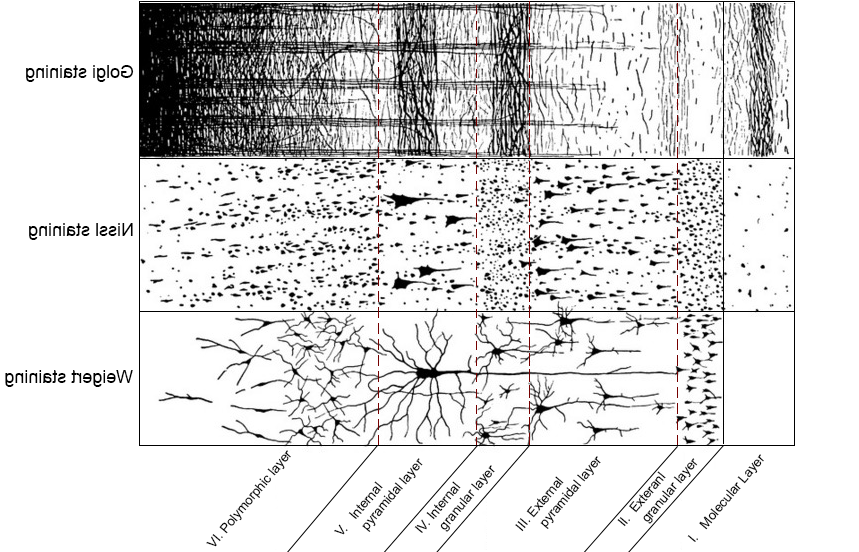
\includegraphics[width=0.8\textwidth, clip=true]{./Chapters/01_Introduction/Images/Layers}
	\caption{\cite{Brodman1909} }
	\label{fig:layers}
\end{figure}

For a small set of experiments, it is relatively straightforward to say if they are feed forward or feedback, but now think of more complicated processes: what would constitute as feed forward in language processing, decision making or memory? This is largely unknown and that is why it is of great interest to learn more about the laminar processing. It could shed light on a multitude of cognitive processes and open doors to a whole new type of information and new research in the brain \cite{Lawrence2017}. However, the greatest barrier is that is neuronal communication is not easily measured. With fMRI, only a derivative of neuronal firing can be measured as changes in oxygen consumption. We will therefore first need to get a better understanding of what type of information it is that fMRI can yield.

\section{Contrast Mechanisms}
Neurons clearly have layer specific functions, but measuring them is not easy, especially not in living humans. We cannot put electrodes in their heads, but what we can do is put them in an MRI scanner. An MRI scanner, however, cannot measure direct neuronal firing. Instead, it is susceptible to all kinds of magnetic properties of which three dimensional images can be made. Most notably, the magnetic susceptibility of red blood cells changes when they are oxygen rich or oxygen poor \cite{Ogawa1990}, which we call the Blood Oxygenation Level Dependant Signal, the BOLD signal. However, while there is little doubt that activation in a cortical region elicits a BOLD response, large parts of the biological mechanism behind it are still disputed. Most importantly, the extent to which the BOLD response reflects laminar specific activation is largely unknown. 

It was noted that maybe more so than just activity (MUA, multi unit acitvity), the amount of synaptic input (measured by the local field potential, LFP) migth be crucial for the strength of the BOLD response \cite{Goense2008}.

\begin{figure}[!ht]
	\centering
	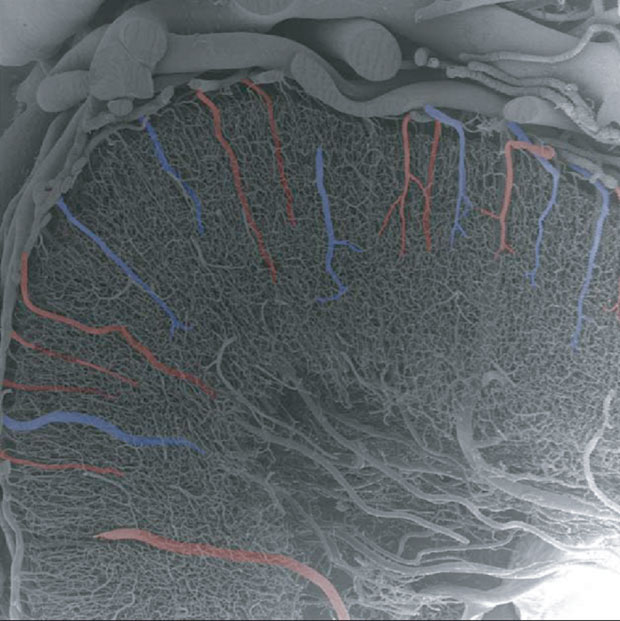
\includegraphics[width=0.9\textwidth, clip=true]{./Chapters/01_Introduction/Images/Microvasculature}
	\caption{The microvasculature of the visual cortex of a macaque \cite{Weber2008}. }
	\label{fig:microvasulature}
\end{figure}
Figure~\ref{fig:microvasulature} shows the microvasculature of a small piece of visual cortex in a macaque. In red, the arterioles, small blood vessels that dive from the top of the cortex (the pial surface) downward to supply the whole grey matter from blood. The smallest vessels, the capillaries, relay the oxygen to the neurons in all cortical layers, such that deoxygenated hemoglobin is drained away by the veins (blue). The veins on top of the cortex can be an order of magnitude larger than the cortical veins, and conduct off the deoxygenated blood. This might make one appreciate the difficulty of extracting laminar specific signals with large signals of non-interest in the direct neighbourhood. 

But the level of blood oxygenation is not the only quantity that fluctuates as a result of cortical activation. More blood starts flowing (higher cerebral blood flow, CBF), vessels start dilating (more cerebral blood volume, CBV) and the consumption of oxygen increases (higher cerebral metabolic rate of oxygen, CMR$_{O2}$). These quantitative measures can be related to one another by the Davis model, save some free parameters that need to be empirically determined \cite{Davis1997}. However, the proposed equations hold for the cortical column in its entirety, but does not take into account potential layer specific differences. 

So while we cannot measure neuronal activation with MRI, the closest we can get is the traces in the magnetic properties in the vasculature through BOLD, CBV, CBF, and CMRO$_{2}$. The extent to which these quantities vary as spatially specific as the level of the cortical layers is an outstanding question, however, and needs to empiraclly tested. Indeed, there are techniques to measure them, $T_2^*$-weighted imaging \cite{Norris2006} for BOLD, VASO for CBV \cite{Huber2018}, arterial spin labelling \cite{Grade2015} for CBV, and calibrated BOLD \cite{Blockley2013}) for CMRO$_{2}$. All vary in terms of sensitivity, specificity, and attainable resolution (spatial as well as temporal). The spatial resolution in combination with the type of experiment that is required for CBF and CMRO$_2$ measurements makes them poor candidates for human in vivo fMRI. It is mainly BOLD and CBV that have shown promising layer specific differences in animal experiments \cite{Lu2004,Zhao2006,Jin2008,Goense2012}. The main benefits of VASO compared to BOLD are its quantifiability \cite{Lu2003} and local specificity \cite{Jin2006}, whereas BOLD has higher sensitivity and speed \cite{Huber2018}.

Our main goal was to investigate the possibilities of laminar analysis in standard experiments on humans, and hence chose to use the BOLD signal as our signal of interest. Fundamentally, the BOLD signal arises as a consequence of magnetic field perturbations arising from desoxyhemoglobin molecules \cite{Norris2006}. These changes extend beyond the blood vessel and drop off as a function of field strength, the orientation of the vessel, and the vessel diameter. 
From the time that the molecules are excited until the time of the echo, molecules move around through the vessel. If the trajectory of a molecule in this time is small compared to the vessel size (and hence compared to the drop-off), there is little change in its surrounding magnetic field and the effect is reversible, a static effect. If on the other hand the molecule's trajectory is large, its surrounding magnetic field changes more drastically and unpredictably, such that the effect is irreversible and dynamic.
These two contrast mechanisms are the static and dynamic extravascular effect
The magnetic field perturbations scale linearly with field strength, so the trajectory of a molecule relative to the perturbations is much greater at 7 Tesla than at 1.5 Tesla. Thus, the dynamic extravascular effect increase with field strength. 
The remaining static effect at 7 Tesla is thus very specific, but detecting it requires high sensitivity \cite{Panchuelo2014}. 
An additional source of BOLD contrast is the intravascular effect. The magnetic field inside the vessel is slightly different from the surrounding tissue because of the amount of desoxyhemoglobin. As a result, the signal will start to dephase with respect to the extravascular signal. This is can be reversed because it is constant over time and is called the static intravascular effect. The exact origin of the last contrast mechanism is unclear. This is irreversible (dynamic) intravascular dephasing and has to do with the random movement of water molecules within red blood cells. It is either due to these water molecules interacting with the deoxyhemoglobin, or with the diffusion in and out of the cells, but no experiment to date has been able to tease the two mechanisms apart.
Four different contrast mechanisms can be distinguished.

Even given these four contrast mechanisms, it is still an outstanding question in what proportions they proliferate in measurements. This may even vary at the laminar level, as the deoxyhemoglobin from deeper layers flows upward to the top layers. The strengths of these effects have been modelled \cite{Markuerkiaga2016,Uludag2017} for both spin echo and gradient echo and suggest that most of the signal produced in a layer is also visible in that layer. For spin echo this is almost fully the case, while gradient echo has a tail that extents to more superficial layers, but at a gain of sensitivity. A range of laminar profiles has been found using spin echo (e.g. \cite{Zhao2004,Harel2006,Goense2006}), gradient echo (e.g. \cite{Polimeni2010,DeMartino2013,Chen2013}) or a combination of both, GRadient A Spin Echo (GRASE) \cite{Olman2012,DeMartino2013}.

Choosing a sequence requires carefully balancing the advantages and disadvantages against each other. We here chose to use gradient echo to investigate the laminar BOLD signal for its higher sensitivity at a field strength of 7 Tesla for high specificity. The potential downside of this is the susceptibility to the larger veins on top of the cortex that might obscure smaller effects \cite{Barth2007}. While the exact origins of the BOLD signal are unknown, there is strong evidence that the BOLD signal has a laminar footprint \cite{Logothetis2001}. Although some results from animal studies suggest that the effects may be visible at a higher temporal resolution than human in vivo MRI can achieve \cite{Yu2014,OHerron2016}. With the many uncertainties and the small size of the potential effect, it is soon clear that any potential effect can only be picked up with powerful methods that address as many sources of noise as possible. 

\subsection{Methods}
After covering the fundamentals of measurement techniques, it is clear what types of information may be expected to be present in the data. Getting out the relevant information, however, is at least as complicated. The brain is a highly convoluted structure that we are trying to describe and visualise by means of cubic voxel rasters. The first problem we encounter is a geometrical one: how do we attach a brain location to voxels in space? This can be done by making a \emph{cortical reconstruction} on a high resolution brain scan \cite{Dale1999,Bazin2012} with a very clear contrast between the white matter and grey matter as seen in Figure~\ref{fig:mybrain}. The distinction between white and grey matter is clear enough to draw a three dimensional boundary on both side of the grey matter: on the white matter boundary and one on the pial surface, the separation between the grey matter and the cerebrospinal fluid (CSF).
\begin{figure}[!ht]
	\centering
	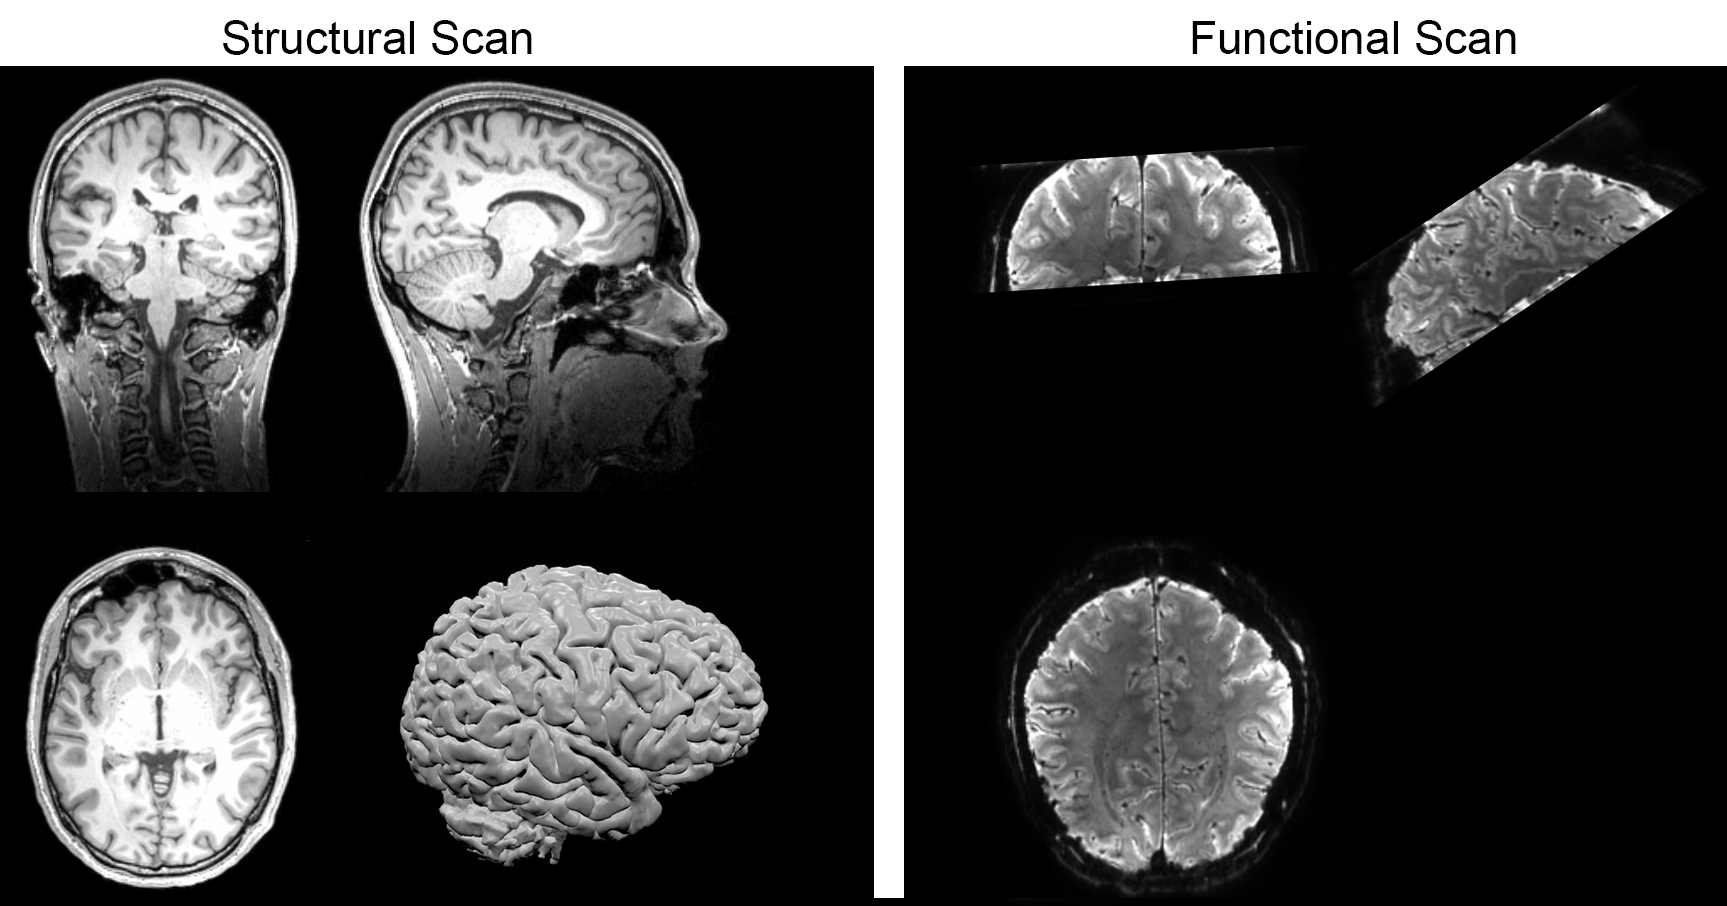
\includegraphics[width=0.99\textwidth, clip=true]{./Chapters/01_Introduction/Images/MyBrain}
	\caption{An example of a structural and functional brain scan. On the left, the structural scan has high anatomical contrast and sharp differences between the white matter and grey matter. The contrast is sharp enough to make a three dimensional reconstruction of the brain (lower right corner). On the right, a functional image is shown. The anatomical contrast is much weaker, but it can be acquired quickly and the contrast is susceptible to slight changes in blood deoxyhemoglobin, related to oxygen consumption on neuronal activation.}
	\label{fig:mybrain}
\end{figure}

The cortical reconstruction is very informative about the shape of the brain and potentially also about the layers: One could imagine different layers to be described as intermediate surfaces between both outer boundaries of which the locations can be used to then sample the cortical layers \cite{Koopmans2011,Polimeni2010,DeMartino2013}.
This descriptions allows for all sorts of surface base calculations \cite{Fischl2000,Bazin2012} and for example allows us to take into account a more naturalistic flow of the cortical layers \cite{Bok1929,Waehnertr2014}. Here it is described 



The people that we scan will move, breathe, fall asleep, ca
The scanner 


When we talk about a scanner with a field strength of 7 Tesla, it means there should be a homogeneous static magnetic field of that strength in the centre of the scanner. However, because the presence of a human body perturbs the field, it is not as homogeneous as one might want. Small perturbations can be corrected by \emph{shimming}, applying an additional magnetic field to compensate for the inhomogeneities. However, this is not accurate enough to correct all deviations and the inhomogeneities need not be constant over time. 


Distortion. The magnetic field is not always homogeneous



Multiple types 


It is possible geometrical properties 


%%
Balloon model \cite{Buxton1998}
something with a dynamic model of the hemodynamic signal \cite{Friston2000}.
















\section*{Thesis outline}
This thesis covers two major problems in laminar fMRI that needed to be solved before an experimental study could be conducted, and will reflect on building an fMRI pipeline, laminar or otherwise. In Chapter~\ref{ch:registration}, we will discuss a new way of coregistering an anatomical scan with a functional scan, when the latter is non-linearly distorted. We explain the details of the distortion correction technique, show its performance, and freely provide the code and data online. Chapter~\ref{ch:glm} describes a novel way of extracting laminar signal from data. We show its performance on a multitude of data, from a simulated fMRI model to post mortem data, to in vivo data from a set of subjects. Having overcome several of the most challenging aspects of laminar analysis, we then proceed to a laminar experiment in Chapter~\ref{ch:attention}. In a visual attention experiment, we investigate the laminar response. We further developped a new tool to more easily build fMRI analysis pipeline, to more reprodicibly conduct science, and to easily share analysis pipelines with others in Chapter~\ref{ch:porcupine}. Finally, these results will be put in a broader perspective in the Discussion, Chapter~\ref{ch:discussion}.


\linespread{1.5}
\newpage

%\linenumbers
%\afterpage{\blankpage}
\chapter{Preserved Spontaneous Mentalizing amid Reduced Intersubject Variability in Autism during a Movie Narrative}
\label{ch:mentalizing_asc}

\begin{center}
    \large\textit{Abstract}
\end{center} 

{\abstractfont 
While individuals with autism often face challenges in everyday social interactions, they may demonstrate proficiency in structured mentalizing tasks that assess their ability to infer others' mental states. Using functional MRI and pupillometry, we investigated whether these discrepancies stem from diminished spontaneous mentalizing or broader difficulties in unstructured contexts. Fifty-two adults diagnosed with autism and 52 neurotypical controls viewed 'Partly Cloudy', a nonverbal animated film with a dynamic social narrative known to engage the mentalizing brain network during specific scenes. Analysis focused on comparing brain and pupil responses to these mentalizing events. Additionally, dynamic intersubject correlations explored the variability of these responses throughout the film. Both groups showed similar brain and pupil responses to mentalizing events and provided comparable descriptions of the characters' mental states. However, participants with autism exhibited significantly stronger correlations in their responses across the film's social narrative, indicating reduced inter-individual variability. This distinct pattern emerged well before any mentalizing events and involved brain regions beyond the mentalizing network. Our findings provide functional evidence of spontaneous mentalizing in autism, demonstrating this capacity in a context affording but not requiring mentalizing. Rather than responses to mentalizing events, a novel neurocognitive signature - inter-individual variability in brain and pupil responses to evolving social narratives - differentiated neurotypical individuals from those with autism. These results suggest that idiosyncratic narrative processing in unstructured settings, a common element of everyday social interactions, may offer a more sensitive scenario for understanding the autistic mind. \par
} 

\vspace*{\fill} 
This chapter is adapted from: \bibentry{mangnus2024bpcnni}

\thispagestyle{empty}

\newpage

\section{Introduction}
Autism Spectrum Condition (ASC) is a neurodevelopmental disorder marked by difficulties in social communication and interaction across multiple contexts \citep{apa2013}. These difficulties are frequently associated with mentalizing - the ability to attribute mental states to oneself and others \citep{premack1978,wimmer1983}. While initial findings suggested diminished mentalizing abilities in autism \citep{baron-cohen1985,happe1994}, subsequent studies have painted a more complex picture, owing to a variety of factors.

First, the reliability of established mentalizing assessments, such as the False Belief Test, Strange Stories, and the Reading the Mind in the Eyes Test, has increasingly come under scrutiny. These tests have shown inconsistent effect sizes when compared to earlier, smaller-scale studies and exhibit limited correlations with one another, despite their aim to measure similar or identical mentalizing constructs \citep{gernsbacher2019,higgins2024,schaafsma2015,yeung2024}. Second, many studies do not adequately match autistic individuals with neurotypical controls based on language abilities, which are crucial to varying degrees for these tasks \citep{betz2019}. This lack in language matching is particularly significant given the generally lower performance in verbal learning and memory observed within the autism population \citep{velikonja2019}. Lastly, recent research highlights the remarkable proficiency of autistic individuals in mentalizing tasks, especially in situations requiring strategic mental state reasoning \citep{bowler1992,pantelis2017}, such as deception \citep{vantiel2021}.

Faced with these empirical challenges, researchers have turned to more implicit mentalizing measures. This includes the analysis of anticipatory eye movements concerning an actor's false beliefs \citep{senju2009}, and measuring neural activity in the Animated Triangles task, where participants attribute mental states to moving shapes \citep{abell2000}. Recent findings indicate that while autistic individuals do show anticipatory gaze responses, these responses tend to be generally slower, regardless of whether the character's beliefs were true or false \citep{glenwright2021,schuwerk2016}. In the Animated Triangles task, both autistic and neurotypical participants show comparable brain activation in key mentalizing regions, such as the medial prefrontal cortex (mPFC), temporoparietal junction (TPJ), and precuneus \citep{moessnang2020}. However, individuals with autism typically underperform in both the mentalizing and non-mentalizing conditions of this task, which, combined with their generally slower anticipatory gaze responses, points to broader difficulties in implicit task settings \citep{wilson2021}. The extent to which autistic individuals engage in spontaneous mentalizing, particularly in unstructured settings lacking an explicitly defined task, as is common in everyday social interactions, remains largely unknown.

In this study combining fMRI and pupillometry, we aimed to bridge this knowledge gap by investigating how individuals with and without autism respond to mental state events embedded in a dynamic movie narrative. Additionally, we sought to provide insights into how these individuals process stimuli in less structured environments that more closely resemble everyday social interactions. Everyday interactions require a continuous assessment of stimuli within an evolving narrative \citep{goffman1974,johnson2023,stolk2022}, as seen in how even seemingly minor behaviors like a voluntary cough or a brief silence can carry significant implications in certain contexts \citep{kendon1994}. Failure to recognize these narrative cues could lead to misunderstandings in scenarios that require high levels of interpretation, such as irony or sarcasm, areas known to pose challenges for autistic individuals \citep{deliens2018,zalla2014}. However, capturing this narrative processing is challenging, as it likely unfolds differently over time among individuals exposed to the same stimuli. We reasoned that narrative processing could manifest as inter-individual variability in responses to movie stimuli, particularly diminished among those less inclined to interpret stimuli through a narrative lens \citep{chang2021,finn2018,owen2023,zhang2022}. We investigated this possibility using intersubject correlation analysis \citep{hasson2004}, applying it to two complementary methods for assessing cognitive processing: brain imaging and measurements of pupil size \citep{beatty1982}. 

To probe spontaneous mentalizing and narrative processing, we recorded participants' brain and pupil responses as they viewed the nonverbal animated movie `Partly Cloudy'\citep{jacoby2016,paunov2019}. Although movies cannot fully replicate the complexities of real-world social interactions \citep{wheatley2019}, they offer an effective platform for immersing participants in an evolving narrative under uniform stimulus conditions. To assess differences in narrative processing between autistic and neurotypical participants at various points during the movie, we augmented our intersubject correlation analysis with a dynamic sliding window technique and an adaptive clustering algorithm \citep{maris2007}. The movie Partly Cloudy was chosen for its proven ability to evoke neural activations within the mentalizing network through distinct mental state events \citep{jacoby2016,richardson2018}, making it suitable for evaluating spontaneous mentalizing. After viewing, we analyzed participants' verbal descriptions of the movie, focusing on their use of language related to mental states. This experimental approach enabled us to simultaneously probe spontaneous mentalizing and narrative processing, providing insights into how these cognitive functions interact in individuals with autism.

\section{Materials and methods}
\subsection{Preregistration and Data availability}
The study comprised two sets of preregistered analyses \citep{mangnus2022}. The first set focused on spontaneous pupil and brain responses to movie events anticipated to elicit mental state inferences, complemented by a questionnaire that examined participants' use of related vocabulary in describing the movie. The second set of analyses explored dynamic intersubject correlations to investigate idiosyncratic narrative processing throughout the entire movie. Unlike the event-related analyses, these exploratory analyses were not limited to specific movie segments. All resulting pupillometry and fMRI data are publicly available for further research \citep{mangnus2024dataset}. 

\subsection{Participants} 
The study enrolled 104 participants, divided equally into 52 adults diagnosed with Autism Spectrum Disorder (ASC) and 52 neurotypical controls (NT). Recruitment occurred through Radboud University's database, social media, campus postings, and outpatient clinics in Nijmegen and Arnhem, the Netherlands. Eligibility for the ASC group required a formal diagnosis from a clinician \citep{apa2013}, while exclusion criteria for all included the use of psychotropic drugs, severe cognitive impairment, systemic diseases, or neurological treatment history. As shown in Table~\ref{tab:ppt-stats-asc}, both groups were demographically matched for gender, age (Kullback-Leibler divergence = .05, \textit{F}-test (102) = .29), and both verbal and nonverbal IQ, verified through the Similarities and Vocabulary subscales of the Wechsler Adult Intelligence Scale (WAIS-III \citep{wechsler1997}; KL = .02, \textit{F}-test = .74) and Raven's Progressive Matrices (RPM \citep{raven1989}; KL = .01, \textit{F}-test (102) = .63). ASC participants notably scored higher on the Autism-Spectrum Quotient (AQ-50 \citep{baron-cohen2001AQ}), confirming group distinctions. Data collection involved MRI scans (\textit{n} = 104) and pupillometry (\textit{n} = 100) while participants viewed the film, followed by a post-viewing questionnaire completed by most (\textit{n} = 101). All participants provided written informed consent, approved by the local ethics committee (CMO region Arnhem-Nijmegen, file number 2019-6059), and received compensation for participation.

\begin{table}[ht]
    \captionsetup{justification=raggedright, singlelinecheck=false, font = normal} % Left-align the caption
    \caption{Demographic data}
    \label{tab:ppt-stats-asc}
    \setlength{\tabcolsep}{10pt}
    \renewcommand{\arraystretch}{1.5} % Adjust row spacing (default is 1.0)
    \begin{tabular}{llll}
    \hline
    \textbf{} & \textit{ASC Group} & \textit{NT Group} & \textit{Group Difference} \\
    \hline
    N (men:women) & 52 (23:29) & 52 (20:32) & \textit{$\chi$\textsuperscript{2}}(1, \textit{N} = 104) = 1.73, \textit{p} = .19 \\
    Age (years) & 27.7 (6.3) & 25.9 (5.5) & \textit{t}(102) = 1.74, \textit{p} = .08 \\
    Verbal IQ (WAIS-III) & 126 (16) & 124 (16) & \textit{t}(102) = 0.51, \textit{p} = .61 \\
    Nonverbal IQ (RPM) & 103 (9) & 104 (11) & \textit{t}(102) = -0.46, \textit{p} = .64 \\
    Autism Quotient & 31 (9) & 12 (6) & \textit{t}(102) = 12.2, \textit{p} < .001 \\
    \hline
    \multicolumn{4}{l}{\small{Values are given as Mean (Standard Deviation). ASC, Autism Spectrum Condition; NT, Neurotypical.}} \\
    \end{tabular}
\end{table}
    

\subsection{Experimental design }
Participants watched the 5-minute and 45-second animated short Partly Cloudy, depicting the evolving friendship between a stork and a cloud through various social interactions integral to its narrative. After viewing, they described the plot to assess narrative comprehension and articulation of characters' mental states. Descriptions were analyzed by independent raters, categorizing words into mental state terms or other content-related categories, using the mental state word list from \cite{bang2013}. An independent \textit{t}-test compared the frequency of mental state words used between groups. The movie featured three types of events, coded by the original research team that introduced it as a mentalizing localizer task \citep{jacoby2016}. These included \textit{Mental}, \textit{Pain}, and \textit{Control} events, each annotated on the movie's timeline in Fig~\ref{fig:task-fig-asc}. \textit{Mental} events, totaling 44 seconds across 4 events, were expected to elicit inferences about characters' mental states, depicting scenarios like characters feeling distressed while observing others enjoy a cheerful interaction or mistakenly perceiving betrayal by a friend. \textit{Pain} events, totaling 26 seconds across 7 events, depicted instances where characters experienced physical discomfort, such as being shocked by an eel or bitten by a crocodile. \textit{Control} events, totaling 24 seconds across 3 events, showcased serene moments like birds in flights or panoramic views of clouds. As detailed in later sections, these categorizations facilitated the analysis of mentalizing-related pupillary and neural responses.

\begin{figure}[!ht]
	\centering
    \makebox[\textwidth][c]{\includegraphics[width=1.05\textwidth]{./Chapters/02_MentalizingASC/Images/TaskFig.eps}}
	\caption{Autistic and neurotypical participants viewed a six-minute animated movie portraying the evolving friendship between a stork and a cloud, while their pupil and brain responses were recorded. Originally used by Jacoby et al. (2016) as a Theory of Mind localizer, the movie includes three types of events: Mental, Pain and Control, each marked on the movie timeline. Mental and Pain events were expected to prompt inferences about characters' mental and physical states, whereas Control events featured no characters in the foreground. The event images shown were generated using Copilot in Bing for copyright purposes to closely resemble scenes from the movie.}
    \vspace*{-10pt}
	\label{fig:task-fig}
\end{figure}

%[width=.9\textwidth]



\subsection{Pupillometry and MRI data acquisition}
Pupil size was continuously tracked using an Eyelink 1000 plus eyetracker at 1000 Hz. MRI data were acquired using a Siemens 3T MRI-scanner with a 32-channel head coil. Structural images were obtained with a T1 MPRAGE sequence (TR = 2200 ms, TI = 1100 ms, TE = 2.6 ms, flip angle = 11\textdegree, 
voxel size = 0.8 mm\textsuperscript{3}, acceleration factor = 2). Functional images were acquired with a multi-band multi-echo sequence (TR = 1500 ms, TE = 13.4/34.8/56.2 ms, flip angle = 75\textdegree, voxel size = 2.5 mm\textsuperscript{3}, acceleration factor = 2). Analysis of head movement through framewise displacement (FD) showed no significant differences between the ASC and NT groups. Mean FD was 0.15 \textpm{}{} 0.05 for ASC and 0.16 \textpm{}{} 0.09 for NT (M \textpm{} SD; \textit{t}(102) = -0.78, \textit{p} = .43), with maximum FD values at 0.81 \textpm{} 0.79 for ASC and 1.03 \textpm{} 1.31 for NT (\textit{t}(102) = -1.09, \textit{p} = .28). Additionally, assessments of total head motion, calculated from translation and rotation during the realignment process, indicated no significant differences (Translation: 109.5 \textpm{} 74.6 vs. 114.3 \textpm{} 99.5, \textit{t}(102) = 0.28, \textit{p} = .78; Rotation: 2.0 \textpm{} 0.98 vs. 2.2 \textpm{} 1.2 , \textit{t}(102) = 0.74, \textit{p} = .46).

\subsection{Pupillometry data analysis}
Pupillometry data underwent preprocessing with a combination of established and custom MATLAB routines. Blinks were removed using a noise-based detection algorithm \citep{hershman2018}. Squints, marked by unusually small pupil sizes \citep{mathot2018}, and gaze jumps, indicative of excessive translational eye movements, were both identified and eliminated through visual inspection. After these adjustments, 89.3\% \textpm{} 9.4\% of the data remained usable for the ASC group and 88.4\% \textpm{} 10.6\% for the NT group (\textit{t}(98) = 0.48, \textit{p} = .63). Fixations and saccades were distinguished using an adaptive velocity threshold \citep{nystrom2010}. Pupil timeseries were normalized (\textit{z}-scored) and adjusted for global luminance fluctuations modeled using the \textit{lm()} function from the R \textit{stats} package \citep{bates2015} up to the 5th polynomial order, validated with data from five randomly selected participants. Luminance was quantified using RGB values based on the Rec. 709 formula \citep{itu2002}. 

Event-related pupil responses were analyzed through a 3x2 mixed-design ANOVA with mean pupil size as the dependent variable, and event conditions (\textit{Mental, Pain, Control}) and participant group status (ASC, NT) as factors. Tukey's Honest Significant Difference tests further investigated mentalizing-related contrasts, specifically comparing \textit{Mental} to both \textit{Pain} and \textit{Control} conditions. To verify the robustness of our findings against variations in event timing, a control analysis was conducted by incorporating an additional time-based regressor into the \textit{lm()} function during preprocessing. This adjustment, which incremented by one every second, did not influence the main findings.

Intersubject variability was assessed using dynamic intersubject correlation analysis of the pupil timeseries. Employing a leave-one-out approach, each participant's timeseries was correlated with the composite average timeseries of all other group members \citep{nastase2019}. This analysis was conducted using a 30-second sliding window at 100 ms intervals, generating a correlation timeseries for the entire movie duration per participant. All correlation timeseries were Fisher \textit{z}-transformed and subjected to a nonparametric cluster-based permutation test \citep{maris2007}. This test addresses the multiple comparisons problem in timeseries analysis by clustering significant neighboring data points. These clusters are tested against a null distribution formed by randomly shuffling participant labels and recalculating statistics, allowing the identification of specific timepoints where significant differences in pupil response variability between groups occurred, while effectively controlling for false positives. Statistical testing was performed using a two-sided independent samples \textit{t}-test with 10,000 permutations to establish the null distribution. Clusters that reached a Monte-Carlo \textit{p}-value of .05 or less were considered statistically significant.

\subsection{fMRI data analysis}
Functional images were preprocessed using SPM12, initially consolidating multiple echoes into single volumes through echo-weighted combinations. These volumes were realigned to the initial image using rigid-body transformations and 2nd degree B-spline interpolation, and subsequently unwarped with participant-specific fieldmaps to minimize spatial distortions and signal dropout. Anatomical images were coregistered to the mean functional image and segmented into gray matter, white matter, and cerebral spinal fluid categories using SPM's tissue probability maps, enabling normalization to MNI space. An 8 mm full-width at half-maximum kernel was applied or spatial smoothing. First-level regressors estimated activations for \textit{Mental, Pain,} and \textit{Control} events, and included adjustments for head movement (using squared and cubic terms, along with first and second derivatives) and tissue signal intensities. A 0.6 threshold masking was applied to ensure optimal brain coverage.

Two 2-by-2 mixed-design ANOVAs were conducted to analyze mentalizing activations across \textit{Mental, Pain,} and \textit{Control} conditions and participant groups (ASC, NT). The first contrast (\textit{Mental} > \textit{Pain}) sought to confirm previous findings of enhanced mentalizing network activity \citep{jacoby2016}, while the second (\textit{Mental} > \textit{Control}) extended these findings to scenes lacking foreground characters. Results were subjected to whole-brain, cluster-level correction (\textit{p\textsubscript{FWE}} < .05), with anatomical locations identified using the SPM Anatomy Toolbox \citep{eickhoff2005}. Additionally, a region of interest (ROI) analysis focused on three peak brain regions, complemented by Bayesian analysis \citep{jasp2022} to evaluate consistent neural activation within the mentalizing network across groups, reporting evidence with Bayes Factors (BFs). Robustness against event timing variations was confirmed through a control analysis adding a first-level regressor that incremented with each volume.

Intersubject variability at the neural level was assessed using dynamic intersubject correlation analysis of voxel timeseries, adjusted for head movement and tissue signals. Mirroring the pupillometry analysis, a leave-one-out and sliding window method generated whole-brain correlation timeseries for each participant. For computational efficiency, the data were spatially and temporally downsampled by a factor of three, resulting in a voxel resolution of 7.5 mm and a sampling interval of 4.5 seconds. These data underwent a nonparametric cluster-based permutation test \citep{maris2007}, which corrected for multiple comparisons across voxels and timepoints using a two-sided independent samples \textit{t}-test with 10,000 permutations (Monte-Carlo \textit{p} < .05). The analysis was further refined with a spatially adaptive clustering algorithm, identifying variations in brain response patterns between groups. The spatial distribution of the identified spatiotemporal brain cluster was visualized by summing t-values across all timepoints, producing a three-dimensional representation of significant variability. The degree of overlap between this cluster and the mentalizing network was quantified by comparing their spatial volumes. Lastly, a supplementary analysis without the sliding window approach calculated correlations across the entire voxel timeseries, pinpointing a smaller cluster in the left supramarginal gyrus. In line with the main findings, this cluster demonstrated reduced intersubject variability in the ASC group.

\section{Results}
\subsection{Post-viewing movie descriptions }
After the film viewing, participants were asked to recount the story of the stork and cloud's evolving friendship in their own words. We analyzed these descriptions for the use of mental state words and other content-related terms (Fig~\ref{fig:beh-pupil-asc}a). Statistical analysis revealed no significant differences in the frequency of mental state word usage between the autistic and neurotypical participants (M\textsubscript{ASC} = 0.063, M\textsubscript{NT} = 0.054, \textit{t}(99) = 0.84, \textit{p} = .40; Fig. 2b), with a Bayes Factor in favor of the null hypothesis (BF\textsubscript{Null} = 3.49). This finding suggests that both autistic and neurotypical groups engaged similarly with the mental states depicted in the film.

\begin{figure}[!ht]
    \vspace*{10pt}
	\centering
    \makebox[\textwidth][c]{\includegraphics[width=1.05\textwidth]{./Chapters/02_MentalizingASC/Images/BehPupil.eps}}
	\caption{Comparable mental state descriptions and pupil responses across groups. (a) Word Cloud depicting the frequency of mental state-related vocabulary used by participants in their post-viewing movie descriptions. The size of each word corresponds to its frequency of use. (b) Bar graphs displaying the ratio of mental state words to other content-related terms in these descriptions, showing no significant differences between the two groups. (c) Pupil responses across all event conditions, revealing similar response patterns in both autistic and neurotypical groups. Asterisks denote significant differences between event conditions (all \textit{p} < .001), with no significant differences observed between groups. Outliers are represented by dots, while whiskers display a 1.5 inter-quartile range.}
    \vspace*{-10pt}
	\label{fig:beh-pupil-asc}
\end{figure}



\subsection{Event-related pupil responses}
Participants' pupil sizes were continuously tracked throughout the movie to assess responses to events expected to elicit mental state inferences, such as the cloud reflecting on the stork's actions. We also analyzed responses to events evoking physical state inferences, like the stork experiencing pain, as well as to control scenes devoid of character interactions. Pupillometry analysis identified distinct responses to these three event types (\textit{F}(2,196) = 73.0, \textit{p} < .001, BF\textsubscript{Null} = 0.00; Fig~\ref{fig:beh-pupil-asc}c), with the largest pupil dilation occurring during \textit{Pain} events (M = 0.22, \textit{z}-score), followed by \textit{Mental} events (M = -0.12) and \textit{Control} events (M = -0.20). Comparisons of pupil responses between autistic and neurotypical participants revealed no significant differences (\textit{F}(1,98) = 0.03, \textit{p} = .86, BF\textsubscript{Null} = 7.8), nor were there significant interaction effects between participant groups and event types (\textit{F}(2,196) = 2.1, \textit{p} = .12, BF\textsubscript{Null} = 2.5). This suggests that both groups reacted similarly to the different event types in the movie.

\subsection{Event-related brain responses}
A whole-brain fMRI analysis was conducted to examine neural activations during \textit{Mental} events in comparison to \textit{Control} and \textit{Pain} events. As depicted in Fig~\ref{fig:fmri-results-asc}a, this analysis identified robust activation in keys areas of the mentalizing network \citep{schurz2014}, specifically in the right and left temporoparietal junction (rTPJ: xyz\textsubscript{MNI} = [48, -62, 32], \textit{t} = 16.85, \textit{p\textsubscript{FWE}} < 0.001; lTPJ: [-46, -62, 32], \textit{t} = 16.92, \textit{p\textsubscript{FWE}} < 0.001), the precuneus ([6, -64, 40], \textit{t} = 20.64, \textit{p\textsubscript{FWE}} < 0.001), medial prefrontal cortex (mPFC: [-6, 52, 38], \textit{t} = 7.33, \textit{p\textsubscript{FWE}} < 0.001), and left middle temporal gyrus ([-52, 2, -26], \textit{t} = 11.51, \textit{p\textsubscript{FWE}} < 0.001). Echoing the pupillometry findings, no significant differences in neural activation were observed between autistic and neurotypical participants. Complementary region of interest (ROI) analyses (Fig~\ref{fig:fmri-results-asc}b) and Bayesian analyses reinforced these findings, providing evidence favoring the null hypothesis over alternative models suggesting group differences. This was consistently demonstrated across all evaluated ROIs for both \textit{Mental} > \textit{Pain} contrasts (rTPJ: BF\textsubscript{Null} = 4.83, precuneus: BF\textsubscript{Null} = 1.73, mPFC: BF\textsubscript{Null} = 4.01) and \textit{Mental} > \textit{Control} contrasts (rTPJ: BF\textsubscript{Null} = 3.43, precuneus: BF\textsubscript{Null} = 3.63,  mPFC: BF\textsubscript{Null} = 4.71), underscoring a similarity in neural processing of mental states among autistic and neurotypical individuals.

\begin{figure}[!ht]
	\centering
    \includegraphics[width=1\textwidth,trim={0 9cm 0 0},clip=true]{./Chapters/02_MentalizingASC/Images/FMRIResults.eps}
	\caption{Comparable neural activation patterns during mental state events across groups. (a) Brain sections showing whole-brain responses specific to mental state events, as assessed through the Mental > Control and Mental > Pain contrasts. There were no significant differences in activation for either contrast between the autistic and neurotypical groups. (b) Box plots depicting the contrast estimates for the Mental > Control (in blue) and Mental > Pain (in red) comparisons across various Regions of Interest (ROI) for both groups. rTPJ and mPFC were selected as ROIs based on mentalizing literature, while the precuneus was selected because of the peak voxel being located in that region for both mentalizing contrasts. Across all ROIs and contrasts, no significant differences were observed between the groups. Outliers are represented by dots, while whiskers display a 1.5 inter-quartile range.}
    \vspace*{-10pt}
	\label{fig:fmri-results}
\end{figure}

%\makebox[\textwidth][c]{



\subsection{Movie-driven variability in pupil responses }
Having observed comparable pupil and brain responses to mental state events and similar verbal descriptions from both autistic and neurotypical participants, we expanded our investigation to narrative processing differences across the entire movie through dynamic intersubject correlation analysis of the pupil timeseries. This analysis revealed an interval from 40 to 71 seconds where individuals with autism demonstrated significantly stronger correlations in pupil responses, indicating reduced intersubject variability compared to neurotypical participants (M\textsubscript{ASC} = 0.61, M\textsubscript{NT} = 0.55, \textit{cluster stat} = 777, \textit{p} = .045; Fig~\ref{fig:isc-pupil-asc}). This interval preceded any mental state events and coincided with scenes featuring storks flying through the air and clouds morphing into baby animals. Although this reduced variability continued throughout the film, it did not reach statistical significance outside this interval after adjusting for multiple comparisons. Further, differences in variability were not due to variations in saccadic eye movements, as their frequency and variability remained consistent between groups (Fig~\ref{fig:saccades-suppl}).

\begin{figure}[!ht]
    \vspace*{5pt}
	\centering
    \includegraphics[width=1\textwidth,clip=true]{./Chapters/02_MentalizingASC/Images/ISCPupil.eps}
	\caption{Reduced pupil response variability in autistic participants. Dynamic intersubject correlation analysis initially showed comparably high levels of correlation in both autistic and neurotypical groups at the start of the movie. However, a significant divergence emerged around the 40-second mark, where autistic individuals showed stronger correlations in their pupil responses, indicating reduced intersubject variability, compared to neurotypical participants. This pattern of reduced variability emerged well before the mental state events highlighted in red. Solid lines delineate statistically significant intervals, as determined by a cluster-based permutation test.}
    \vspace*{-15pt}
	\label{fig:isc-pupil-asc}
\end{figure}





\subsection{Movie-driven variability in brain responses}
When applied to the fMRI data, dynamic intersubject correlation analysis identified a spatiotemporal cluster where individuals with autism showed significantly stronger correlations in their brain responses compared to neurotypical participants (Fig~\ref{fig:isc-fmri-time-asc}). This cluster spanned the entire movie (\textit{cluster stat} = 1332, \textit{p} = .002) and included peaks in the right and left supramarginal gyrus (rSMG: xyz\textsubscript{MNI} = [52, -34, 32], \textit{t\textsubscript{max}} = 3.88; lSMG: [-54, -40, 32], \textit{t\textsubscript{max}} = 4.54), the right inferior temporal gyrus (rITG: [54, -22, -28], \textit{t\textsubscript{max}} = 5.90), and the left calcarine gyrus (lCG: [6, -102, -10], \textit{t\textsubscript{max}} = 4.20). The reduced variability was consistent across these regions for most of the movie (Fig~\ref{fig:isc-fmri-peak-suppl}), and it emerged well before and continued after any mental state events. The cluster's overlap with the mentalizing network was minimal, comprising less than 20\% of the total cluster size (Fig~\ref{fig:isc-fmri-overlap-asc}). This indicates that the observed reduced variability in brain responses among autistic participants extends beyond regions involved in mental state processing, suggesting broader differences in neural processing between the groups.

\begin{figure}[!ht]
	\centering
    \makebox[\textwidth][c]{\includegraphics[width=1.05\textwidth,clip=true]{./Chapters/02_MentalizingASC/Images/ISCFMRITime.eps}}
	\caption{Reduced brain response variability in autistic participants. Dynamic intersubject correlation analysis identified a spatiotemporal brain cluster where autistic individuals demonstrated significantly stronger correlations in their brain responses, indicating reduced intersubject variability, compared to neurotypical participants. This cluster persisted throughout the movie and featured peaks in the right and left supramarginal gyrus, the right inferior temporal gyrus, and the left calcarine gyrus. Echoing the pupillometry data, this pattern of reduced variability in autistic participants emerged well before the mental state events highlighted in red. LH, left hemisphere; RH, right hemisphere.}
    \vspace*{-10pt}
	\label{fig:isc-fmri-time-asc}
\end{figure}





\vspace*{.1cm}

\begin{figure}[!ht]
	\centering
    \includegraphics[width=1\textwidth,clip=true]{./Chapters/02_MentalizingASC/Images/ISCFMRIOverlap.eps}
	\caption{Limited spatial overlap between brain regions showing reduced intersubject variability in autistic participants and mentalizing activation. The overlap comprised less than 20\% of the total cluster size. For clarity, the cluster is visualized using a cumulative \textit{t}-value threshold of 20 or higher. Lateral brain images provide an overlay with a search distance of 10 mm. }
    \vspace*{-10pt}
	\label{fig:isc-fmri-overlap}
\end{figure}





\section{Discussion}
Using fMRI and pupillometry, this study provides functional evidence of spontaneous mentalizing abilities in individuals with autism. Compared to neurotypical controls matched for gender, age, and both verbal and nonverbal IQ, individuals with autism exhibited similar brain and pupil responses during movie scenes known to activate the mentalizing network \citep{jacoby2016,richardson2018}. Activity in the mentalizing network was enhanced during scenes that encouraged viewers to contemplate the actions and mental states of depicted characters. Conversely, scenes prompting physical state inferences, such as characters experiencing physical discomfort, or control scenes lacking central characters, resulted in weaker mentalizing activations. Verbal descriptions provided by participants after the movie corroborated these findings, indicating an engagement with the mental state events depicted in the movie on par with that of neurotypical controls. These results extend prior evidence of preserved mentalizing in autism \citep{moessnang2020,dufour2013}, showcasing this capacity in a situation affording but not requiring mentalizing.

While individuals with and without ASC showed comparable brain and pupil responses during mental state events, dynamic intersubject correlation analysis revealed significant differences in the correlation of these responses over extended movie intervals. Participants with autism exhibited significantly stronger correlations, indicating reduced inter-individual variability, across several brain regions outside the mentalizing network. These regions included the right and left supramarginal gyrus, linked to empathic judgment \citep{silani2013,wada2021}, the right inferior temporal gyrus, associated with narrative comprehension \citep{youssofzadeh2022}, and the left calcarine gyrus, crucial for visual processing \citep{woldorff2002}. This reduced variability was not due to differences in bottom-up processing, as both autistic and neurotypical groups exhibited similar saccadic eye movement patterns throughout the film. The most pronounced differences emerged during early scenes featuring storks flying through the air and clouds morphing into baby animals, which likely introduced significant narrative ambiguity. This ambiguity may have prompted neurotypical viewers to idiosyncratically interpret how these visual elements fit into the evolving storyline, resulting in less consistent responses. In contrast, autistic participants' responses appeared to be more consistently aligned with the movie's stimuli, possibly reflecting a heightened focus on specific details rather than the broader narrative context \citep{losh2003,tager-flusberg1995,barnes2012,geelhand2020,koldewyn2014}. Importantly, these differences manifested in cognitive and neural processing rather than in eye movements, suggesting that the variability observed in neurotypical responses may represent a neurocognitive signature of top-down processing.

The neuroanatomical bases of the observed changes in response variability are in line with existing research on autism and social interaction. Prior studies have documented structural alterations in the gray matter of both the right and left supramarginal gyrus in individuals with autism \citep{brieber2007,ke2008,libero2014}, as well as reduced anatomical connectivity in the right inferior temporal cortex \citep{boets2018,koldewyn2014}. This region exhibits prolonged activations during tasks involving story comprehension and interactive communication \citep{youssofzadeh2022,stolk2013neural}, highlighting its role in integrating stimuli within an evolving narrative. This integration is crucial for complex social interactions, which necessitate the continuous assessment of diverse stimuli to maintain narrative coherence with others \citep{goffman1974,johnson2023,stolk2022}. A key direction for future research is to examine how response variability in the identified brain regions differs across various social contexts. Such investigations will not only help to illuminate the specific challenges faced by autistic individuals in everyday social situations, but could also inform the development of interventions by identifying environments that promote effective social interaction \citep{wadge2019}.

It is worth noting that our intersubject correlation patterns differ from previous studies demonstrating greater brain response variability in autistic individuals compared to neurotypicals \citep{byrge2015,hahamy2015,hasson2009,lyons2020,nunes2019,ou2022,pegado2020,salmi2013}. Several factors could explain these discrepancies. First, our study used an animated film with fictional characters, as opposed to the more realistic human portrayals in other studies. Although the type of characters may influence brain responses in autism \citep{atherton2018}, greater neural variability has been noted with fictional characters \citep{lyons2020}. Second, we implemented an adaptive clustering algorithm to identify spatiotemporal clusters of brain response variability within 30-second intervals. This approach is potentially more sensitive to brain response variations associated with subtle shifts in interpretation than whole-movie analyses, which emphasize consistent patterns over significantly longer durations (10 to 67 minutes). This approach may more effectively capture the hypothesized increased reliance on bottom-up sensory stimulation in autism \citep{pellicano2012}, possibly leading to less variability in neural signals related to narrative interpretation. More generally, our findings invite a reconsideration of theories that propose precise neural synchronization as a means to manage individual perspectives in daily interactions \citep{holroyd2022}. These theories suggest that aligning neural responses to external cues helps individuals achieve a common viewpoint, thereby facilitating social interaction \citep{hasson2012,mayo2021}. However, contrary to expectations based on their social difficulties, participants with autism in our study displayed stronger neural correlations when exposed to the same external stimuli, challenging the assumed role of precise neural synchronization in social interaction \citep{stolk2014}.

In conclusion, this study offers functional evidence of spontaneous mentalizing in autism, showcasing this capacity in a context affording but not requiring mental state inferences. More distinctively, our findings identify a novel neurocognitive signature - inter-individual variability in brain and pupil responses to evolving social narratives - that differentiates neurotypical individuals from those with autism. These results underscore the importance of idiosyncratic narrative processing in unstructured settings, a hallmark of everyday social interactions, as a potentially more sensitive framework for understanding the autistic mind.
\newpage  
\section{Supplementary information} 

% table S1. 
\begin{table}[ht]
    \centering
    \captionsetup{justification=raggedright, singlelinecheck=false, font = normal} % Left-align the caption
    \setlength{\tabcolsep}{6pt} % Adjust column spacing if needed
    \renewcommand{\arraystretch}{1.5} % Adjust row spacing
    \caption{Results of the within-subject fMRI analyses related to the main effects of event type (Mental, Pain, Control).}
    \label{tab:fmri_anova}
    \small
    \begin{tabular}{lllccccc}
    \hline
    \textit{Contrast} & \textit{Anatomical location of peak voxel} & \textit{Cluster size} & \multicolumn{3}{c}{\textit{MNI coordinates}} & \textit{T-value} \\
     &  &  & \textit{x} & \textit{y} & \textit{z} & \textit{(df = 1, 102)} \\
    \hline
    Mental > Pain & Right precuneus & 19445 & 6 & -64 & 40 & 20.64 \\
     & Right superior frontal gyrus & 16376 & 28 & 26 & 54 & 12.76 \\
     & Left middle temporal gyrus & 2560 & -52 & 2 & -26 & 11.51 \\
     & Right middle temporal gyrus & 1782 & 60 & -12 & -20 & 10.14 \\
     & Right parahippocampal gyrus & 311 & 22 & -40 & -10 & 5.40 \\
    Mental > Control & Left precuneus & 31320 & -2 & -54 & 44 & 15.25 \\
     & Left middle temporal gyrus & 2525 & -56 & -8 & -20 & 10.58 \\
     & Left superior medial gyrus & 8939 & -6 & 52 & 38 & 7.33 \\
    \hline
    \end{tabular}
    \normalsize
\end{table}
    
\newpage

\begin{figure}[!ht]
	\centering
    \includegraphics[width=1\textwidth,clip=true]{./Chapters/02_MentalizingASC/Images/SaccadesSuppl.eps}
	\caption{Frequency and variability of saccadic eye movements. (a) Mean number of saccades observed throughout the movie in both autistic and neurotypical individuals. No significant differences in the frequency of saccades were detected between the two groups. (b) Mean intersubject correlation coefficients representing the variability in the number of saccades across the movie among autistic and neurotypical individuals. No significant differences in saccade variability were observed between the two groups.}
    \vspace*{-10pt}
	\label{fig:saccades-suppl}
\end{figure}





\newpage

\begin{figure}[!ht]
	\centering
    \includegraphics[width=1\textwidth,clip=true]{./Chapters/02_MentalizingASC/Images/ISCFMRIPeaksSuppl.eps}
	\caption{Brain response variability across four key regions, including the right and left supramarginal gyrus (rSMG; lSMG), the right inferior temporal gyrus (rITG), and the left calcarine gyrus (lCG). \textit{T}-values were extracted from a 30 mm diameter sphere centered on the peak voxel. Variability in all four regions was statistically significant throughout most of the movie duration.}
    \vspace*{-10pt}
	\label{fig:isc-fmri-peak-suppl}
\end{figure}





%\afterpage{\blankpage}
\chapter{Social Anxiety Alters Mentalizing Activation and Intersubject Neural Variability During Movie Viewing}
\label{ch:mentalizing_sa}

\vspace{-1cm}
\begin{center}
    \large\textit{Abstract}
\end{center} 

{\abstractfont 
Social anxiety is characterized by an intense fear of judgment in social situations, yet the underlying mechanisms driving this condition remain poorly understood. One hypothesis holds that specific alterations in mentalizing affect the ability to interpret others' thoughts and emotions. Another hypothesis proposes that broader interpretive biases lead individuals to perceive social cues as overly significant, even in neutral settings. We investigated these possibilities by measuring brain activity, pupil responses, and heart rates in socially anxious individuals and matched controls as they viewed 'Partly Cloudy', an animated film known to engage the mentalizing network during specific scenes. While overall brain activity during mentalizing-related scenes was similar across groups, socially anxious participants exhibited reduced activation in the left posterior superior temporal sulcus (pSTS), a key area for mentalizing processing. Additionally, intersubject correlation analysis revealed a distinct neural response pattern in the socially anxious group, marked by uniform responses in sensory regions and heightened variability in higher-order cortical areas. This pattern persisted throughout the film and occurred without changes in heart rate or pupil responses, indicating a neural processing bias that manifests even in non-evaluative settings. These findings provide a neural basis for mentalizing alterations and broader interpretive biases in social anxiety, supporting cognitive-behavioral models and suggesting novel targets for intervention.
}  

\vspace{2cm}
This chapter is submitted as: \bibentry{mangnus2024social}

\thispagestyle{empty}

\newpage

\section{Introduction}

Social Anxiety Disorder (SAD), also known as social phobia, is defined by an intense and persistent fear of social situations, often manifesting during childhood or adolescence. Affecting approximately 12\% of adults at some point in their lives \citep{kessler2005}, SAD leads individuals to experience excessive worry and to avoid situations where they might be judged or scrutinized, from everyday interactions to high-stakes events like public speaking or job interviews \citep{apa2013}. While avoidance might seem protective, it typically intensifies feelings of isolation and deteriorates overall mental health \citep{lim2016}, highlighting the urgent need for a deeper understanding of the mechanisms behind this anxiety disorder to develop more effective treatments.

This study investigates two hypotheses concerning the underlying mechanisms of social anxiety. The first hypothesis posits that alterations in mentalizing affect individuals' ability to accurately interpret others' thoughts and emotions \citep{hezel2014}, thereby increasing stress and anxiety during social interactions \citep{catalino2012,leary1995}. Evidence indicates that individuals with SAD typically underperform on mentalizing tasks, such as the Reading the Mind in the Eyes Test and the Movie Assessment of Social Cognition, relative to nonclinical controls \citep{alvi2020,baez2023,baron-cohen1997,dziobek2006}. Furthermore, research suggests that individuals with SAD may perceive emotions as more intense than they actually are, raising questions about the potential over- or under-utilization of their mentalizing capabilities \citep{hezel2014,nikolic2019,washburn2016}. Despite these findings, neuroimaging studies exploring mentalizing in the context of social anxiety are limited \citep{sripada2009}. It also remains unclear whether alterations in mentalizing are a constant feature of the disorder or are predominantly triggered by situations imposing explicit task demands and evaluative pressures. Clarifying this distinction could help determine whether these mentalizing changes are inherent to SAD or contextually induced.

The second hypothesis suggests that individuals with SAD possess broader interpretive biases, perceiving social cues as overly significant with profound personal implications \citep{clark1995,rapee1997}. While theoretical models vary, they generally agree that these biases compel individuals to incessantly monitor their environments for potential social evaluative threats \citep{amir1998,constans1999,heimberg2014,hirsch2004information,stopa2000} and to critically assess their own behaviors \citep{rapee1992,stopa1993}. Neuroscientific studies support these theories by demonstrating that feedback from social performance tasks, such as public speaking, elicits negatively biased responses in brain areas like the precuneus and frontoparietal regions, reinforcing a negative self-image \citep{koban2023}. Additionally, research on children with social anxiety shows considerable intersubject variability in these regions when exposed to socioemotionally charged films, suggesting a heightened subjective response to social stimuli even in task-free settings \citep{camacho2023}. Nonetheless, it remains uncertain whether these brain responses are linked to mentalizing processes or reflect distinct interpretive mechanisms. Although activation in these areas hints at potential overlap with the mentalizing network, which includes the medial prefrontal cortex, precuneus, temporoparietal junction, and posterior superior temporal sulcus, direct comparisons of these hypotheses through functional brain imaging have yet to be conducted.

In this study, we employed Pixar's animated short film 'Partly Cloudy' to investigate how individuals with varying levels of social anxiety utilize their mentalizing capabilities in a task-free environment. The film, which portrays the developing friendship and interactions between a stork and a cloud, contains specific scenes known to activate the mentalizing network by illustrating characters' mental states \citep{jacoby2016,paunov2019,richardson2018}. Beyond analyzing responses to these mentalizing-specific scenes, the film's continuously evolving narrative provides an effective platform for assessing individual differences in processing identical stimuli throughout the film using dynamic intersubject correlation analysis. Previous research using this method found reduced intersubject variability in brain and pupil responses among autistic individuals during substantial portions of the film \citep{mangnus2024bpcnni}. This uniformity was primarily observed in brain regions outside the mentalizing network, while the mentalizing network itself exhibited robust responses to scenes depicting mental states in both autistic and non-autistic viewers. These observations highlight the film's utility in examining both mentalizing-specific activation and broader interpretive processing. Leveraging these insights, the current neuroimaging study aims to delineate how these processes interact and manifest in individuals with social anxiety under comparable viewing conditions.

Forty-three socially anxious participants and 43 matched controls viewed the film inside an MRI scanner. To minimize performance-related anxiety, we measured whole-brain activity and pupil responses without providing specific task instructions, and we monitored heart rate to assess physiological arousal levels \citep{wascher2021}. After the viewing, participants completed an unannounced questionnaire evaluating their engagement with the film. Our analysis comprised two primary components. First, we conducted event-related comparisons between groups during scenes that depicted characters' mental states, assessing mentalizing activation in individuals with high and low levels of social anxiety. Based on previous observations of diminished mentalizing performance \citep{baez2023}, we anticipated altered activation within the mentalizing network among socially anxious individuals during these scenes. Second, we analyzed intersubject correlations throughout the film, focusing on sustained variations that could indicate differences in subjective engagement or interpretive biases among socially anxious individuals. Drawing on related research involving children \citep{camacho2023}, we hypothesized that socially anxious participants would show increased intersubject variability in frontoparietal regions associated with socioemotional processing. Because results indicated heightened neural variability in regions previously showing reduced variability in autism, we compared neural patterns between these groups to uncover common and distinct mechanisms underlying social processing in autism and social anxiety \citep{white2009}.


\section{Materials and methods}
\subsection{Participants}
Eighty-six adult participants were recruited through Radboud University's database, social media advertisements, and campus postings. Exclusion criteria included the use of psychotropic or systemic glucocorticoid medications, systemic diseases, severe cognitive impairments, or ongoing neurological treatments. Control participants additionally had no current psychiatric diagnoses. Participants were matched for gender, age, and both verbal and nonverbal IQ scores \citep{raven1989,wechsler1997} (see Table~\ref{tab:ppt-stats-sa}). Social anxiety levels were assessed using the Liebowitz Social Anxiety Scale (LSAS) \citep{liebowitz1987,oakman2003}, a 24-item self-report instrument where participants rated their fear and avoidance behaviors on a Likert scale from zero (none/never) to three (severe/usually) across anxiety-inducing situations (e.g., eating in public, interacting with strangers). A cutoff score of 30 \citep{rytwinski2009} categorized participants into high social anxiety (LSAS $\geq$ 30) and control (LSAS < 30) groups, each comprising 43 individuals. Data collection included MRI scans (\textit{n} = 86), pupillometry (\textit{n} = 75), and heart rate measurements (\textit{n} = 74) while participants viewed the film, followed by a post-viewing questionnaire (\textit{n} = 84). All participants provided written informed consent in accordance with local ethics guidelines (CMO region Arnhem-Nijmegen, the Netherlands, file number 2019-6059) and received compensation for participation.

\begin{table}[ht]
    \captionsetup{justification=raggedright, singlelinecheck=false, font = normal} % Left-align the caption
    \setlength{\tabcolsep}{10pt} % Adjust column spacing if needed
    \renewcommand{\arraystretch}{1.5} % Adjust row spacing
    \caption{Demographic data}
    \label{tab:ppt-stats-sa}
    \begin{tabular}{llll}
    \hline
    \textbf{} & \textit{SA Group} & \textit{CON Group} & \textit{Group Difference} \\
    \hline
    N (men:women) & 43 (16:27) & 43 (18:25) & \textit{$\chi$\textsuperscript{2}}(1, \textit{N} = 86) = -0.05, \textit{p} = .83 \\
    Age (years) & 26.3 (5.9) & 26.0 (5.2) & \textit{t}(84) = 0.23, \textit{p} = .82 \\
    Verbal IQ (WAIS-III) & 124 (14) & 128 (16) & \textit{t}(84) = -1.36, \textit{p} = .17 \\
    Nonverbal IQ (RPM) & 102 (11) & 102 (11) & \textit{t}(84) = -0.23, \textit{p} = .82 \\
    Social Anxiety (LSAS) & 51.4 (18.4) & 15.2 (7.5) & \textit{t}(84) = 11.8, \textit{p} < .001 \\
    \hline
    \multicolumn{4}{l}{\small{Values are given as Mean (Standard Deviation). SA, Social Anxiety; CON, Control.}} \\
    \end{tabular}
\end{table}

\subsection{Experimental protocol} 
Participants watched the nonverbal animated film Partly Cloudy (5 minutes 45 seconds), depicting the developing friendship between a stork and a cloud. The film was annotated for three event types: \textit{Mental} (44 seconds across 4 scenes), \textit{Pain} (26 seconds over 7 scenes), and \textit{Control} (24 seconds across 3 scenes), as shown in Fig~\ref{fig:task-fig-sa} \citep{jacoby2016}. \textit{Mental} events were expected to elicit mentalizing inferences about characters' thoughts and emotions, such as distress or betrayal. \textit{Pain} events depicted physical discomfort, like electric shocks or animal attacks. \textit{Control} events showed neutral content, such as birds in flight or cloudscapes without foreground characters. These categories were used to analyze mentalizing-related brain and pupil responses. Before the MRI session, participants were acclimated to the MRI environment using a dummy scanner to reduce anxiety. After viewing the film, they completed an undisclosed questionnaire describing the plot in their own words. Independent raters analyzed these summaries using a taxonomy of mental state terms \citep{bang2013}, categorizing words referencing mental states and emotions versus general content. An independent \textit{t}-test compared the frequency of mental state-related words between groups. To test for a potential negativity bias among socially anxious participants, a quasi-Poisson regression model assessed the ratio of negative emotion words to the total number of emotion-related words used by each participant.

\begin{figure}[!ht]
	\centering
    \makebox[\textwidth][c]{\includegraphics[width=1.05\textwidth]{./Chapters/03_MentalizingSA/Images/TaskFig.eps}}
	\caption{Socially anxious participants and matched controls viewed the animated short 'Partly Cloudy', which portrays the developing friendship and interactions between a stork and a cloud. During the viewing, participants' pupil responses, brain activity, and heart rates were continuously recorded. The film is annotated to highlight three distinct event types: Mental, Pain and Control, each marked on the film's timeline. Mental events are expected to engage viewers' mentalizing, prompting them to infer the character' thoughts and emotions. Pain events illustrate the characters experiencing physical discomfort, while Control events feature only passive or background imagery. The images displayed were generated using Bing's Copilot to closely replicate scenes from the film, adhering to copyright constraints.}
    \vspace*{-10pt}
	\label{fig:task-fig}
\end{figure}



\subsection{Data acquisition}
During the film screening, heart rate was continuously recorded at 5000 Hz using a finger pulse sensor connected to a BrainAmp ExG MR amplifier (BrainVision software), and pupil diameter was monitored at 1000 Hz using an Eyelink 1000 Plus eye-tracker. MRI scans were conducted on a Siemens 3T scanner with a 32-channel head coil. High-resolution structural images were obtained using a T1 MPRAGE sequence (TR = 2200 ms, TI = 1100 ms, TE = 2.6 ms, flip angle = 11\textdegree, voxel size = 0.8 mm isotropic, and acceleration factor = 2). Functional images were acquired using a multi-band multi-echo sequence (TR = 1500 ms, TEs = 13.4/34.8/56.2 ms, flip angle = 75\textdegree, voxel size = 2.5 mm isotropic, and acceleration factor = 2). Motion analysis revealed no significant differences between socially anxious and control participants in framewise displacement (mean FD = 0.16 \textpm{} 0.08 vs. 0.16 \textpm{} 0.07, \textit{t}(84) = 0.20, \textit{p} = .84; max FD = 0.09 \textpm{} 1.28 vs. 1.15 \textpm{} 1.13, \textit{t}(84) = 0.67, \textit{p} = .51) or total head motion, calculated from translation and rotation parameters during realignment (translation: 118.4 \textpm{} 110.4 vs. 107.4 \textpm{} 78.7, \textit{t}(84) = -0.53, \textit{p} = .59; rotation: 2.3 \textpm{} 2.0 vs. 2.4 \textpm{} 1.9 , \textit{t}(84) = 0.18, \textit{p} = .86).

\subsection{Heart rate analysis}
Heart rate data were preprocessed by removing scanner-induced artifacts using a deconvolution filter from the BrainAmpConverter toolbox. The cleaned signal was then band-pass filtered between 0.2 Hz and 3 Hz to retain biologically relevant frequencies \citep{avram2019}. Heartbeat peaks were detected within 600 ms intervals, and heart rate metrics were derived from the intervals between these peaks. Intersubject variability in heart rate responses was assessed using the dynamic intersubject correlation method described in the pupillometry analysis section (\ref{pupil-methods}).

\subsection{Pupillometry analysis} \label{pupil-methods}
Pupillometry data were preprocessed to extract changes in pupil size, an indicator of cognitive effort \citep{beatty1982}. Blinks and saccades were removed using noise-based detection and adaptive velocity threshold algorithms \citep{hershman2018,nystrom2010}, while visual inspections eliminated squints and gaze jumps \citep{mathot2018}. Each participant's pupil timeseries was standardized (\textit{z}-scored) and adjusted for global luminance variations using a 5th-order polynomial model in R \citep{bates2015}, with luminance derived from RGB values per the Rec. 709 standard \citep{itu2002}. Group differences in mean pupil responses across event types were assessed using a 3x2 mixed-design ANOVA, with event type (\textit{Mental, Pain, Control}) as the within-subject factor and group (socially anxious, control) as the between-subject factor. Significant interaction effects (\textit{p} < .05) were analyzed using Tukey's Honest Significant Difference tests. 

To examine intersubject variability, we conducted dynamic intersubject correlation analysis on the pupil timeseries. Using a leave-one-out method \citep{nastase2019}, each participant's timeseries was correlated with the average of all other group members, applying a 30-second sliding window with 100 ms steps to generate continuous correlation timeseries spanning the entire movie. The correlations were Fisher z-transformed and subjected to a nonparametric cluster-based permutation test to evaluate differences in pupil response variability between groups \citep{maris2007}. This test addresses the multiple comparisons problem in timeseries analysis by aggregating significant adjacent data points into clusters. These clusters are tested against a null distribution formed by randomly shuffling participant labels and reculating statistics, effectively controlling for false positives. Statistical significance was assessed using a two-sided independent samples t-test, with 10,000 permutations. Clusters with a Monte-Carlo \textit{p}-value of .05 or less were considered statistically significant.

\subsection{fMRI analysis}
fMRI data were preprocessed and analyzed using SPM12 (\url{https://www.fil.ion.ucl.ac.uk/spm}). Echoes were merged into a single volume, and images were realigned to the first image using 2nd degree B-spline interpolation with six rigid-body transformation parameters. Spatial distortions were minimized by unwarping images using a fieldmap acquired alongside the functional images. The mean functional images were coregistered with anatomical images and normalized to MNI space using tissue probability maps. Images were then spatially smoothed with an 8 mm full-width at half-maximum kernel. The first-level analysis included regressors for \textit{Mental, Pain,} and \textit{Control} events, end credits, head movement parameters (including squared, cubic terms, and derivatives), and signals from white matter, cerebrospinal fluid, and out-of-brain voxels.

To assess group differences in mentalizing activation, two separate 2x2 mixed-design ANOVAs were conducted. \textit{Mental} and \textit{Pain} events or \textit{Mental} and \textit{Control} events served as within-subject factors, and participant group (socially anxious, control) was the between-subject factor. We hypothesized that these contrasts would reveal common activations within the mentalizing network, isolated using conjunction analysis, and specifically masked to emphasize mentalizing activation in the control group. Results are presented as whole-brain cluster-level corrected effects (p\textsubscript{FWE} < .05, initial cluster-forming threshold at \textit{p} < .001), with anatomical locations identified using the SPM Anatomy Toolbox \citep{eickhoff2005}. A-region of-interest (ROI) analysis focused on key mentalizing-related brain regions, including the right temporoparietal junction (rTPJ), precuneus, and medial prefrontal cortex \citep[mPFC; ][]{schurz2014}, defined by 8 mm radius spheres at peak voxels from the combined mentalizing contrasts. Bayesian analysis assessed variations in mentalizing network activation between groups by calculating Bayes Factors (BFs) to determine the strength of evidence for the null hypothesis versus alternative models \citep{jasp2022}. 

To examine differences in intersubject variability at the neural level, we performed dynamic intersubject correlation analysis on voxel timeseries, adjusted for head movement and tissue signals. Using a combined leave-one-out and sliding-window approach similar to that used in the heart rate and pupillometry analyses, we generated voxel correlation timeseries. For computational efficiency, the data were spatially and temporally downsampled by a factor of three, resulting in a voxel resolution of 7.5 mm and a sampling interval of 4.5 seconds. These data underwent a nonparametric cluster-based permutation test \citep{mangnus2024bpcnni}, correcting for multiple comparisons across voxels and timepoints. To visualize the spatial distributions of identified spatiotemporal clusters, we aggregated the \textit{t}-values across all timepoints, producing a three-dimensional representation highlighting areas with significant variability differences throughout the film's duration. Lastly, we quantified the overlap between the correlation clusters and the mentalizing network by assessing their spatial overlap relative to the total voxel size of the detected clusters.

\section{Results}

\subsection{Post-viewing movie assessment}
After viewing the movie, both socially anxious and matched control participants used a similar frequency of words related to mental states (M\textsubscript{SA} = 0.053, M\textsubscript{CON} = 0.048, \textit{t}(82) = 0.47, \textit{p} =.64; Fig~\ref{fig:beh-pupil-sa}a and b) and emotions (M\textsubscript{SA} = 0.042, M\textsubscript{CON} = 0.034, \textit{t}(82) = 0.74, \textit{p} =.46) when describing the plot. However, socially anxious participants used a significantly lower proportion of negatively charged emotion words (M\textsubscript{SA} = 0.65, M\textsubscript{CON} = 0.85, \textit{t}(50) = -2.61, \textit{p} =.012; Fig~\ref{fig:beh-pupil-sa}c). These results suggest that, although both groups similarly recognized the mental states depicted in the film, socially anxious individuals may have adopted a more positive perspective on the plot upon reflection than their non-anxious counterparts.

\begin{figure}[!ht]
	\centering
    \makebox[\textwidth][c]{\includegraphics[width=1.05\textwidth]{./Chapters/03_MentalizingSA/Images/BehPupil.eps}}
	\caption{(a) Word clouds illustrate the frequency of mental state-related words used by socially anxious and control participants in their movie descriptions. The size of each word is scaled according to its frequency. (b) Proportion of mental state-related words relative to other content words, with no significant differences observed between groups. (c) Proportion of words expressing negative emotions compared to other emotion words, showing a lower incidence of negatively charged words among socially anxious participants relative to controls. (d) Pupil responses across all event types and participants groups, with significant differences between event types marked by asterisks (**\textit{p} < .001, *\textit{p} < .01) and no significant differences between groups. Outliers are represented by dots, while whiskers extend to a 1.5 inter-quartile range.}
    \vspace*{-10pt}
	\label{fig:beh-pupil-sa}
\end{figure}



\subsection{Heart rate responses}
Heart rate, an indicator of physiological arousal \citep{wascher2021}, exhibited significant fluctuations throughout the movie (Fig~\ref{fig:heart-rate}a). However, these changes followed a consistent pattern between socially anxious participants and controls, with no significant differences in heart rate at any point during the film or in average heart rates between the groups (M\textsubscript{SA} = 65.4, M\textsubscript{CON} = 64.0, \textit{t}(72) = 0.62, \textit{p} =.54). Further analysis of intersubject variability in heart rate also showed no significant differences at any point during the film or in average intersubject correlations between the groups (M\textsubscript{SA} = 0.20, M\textsubscript{CON} = 0.20, \textit{t}(72) = 0.10, \textit{p} =.92; Fig~\ref{fig:heart-rate}b). These findings suggest that physiological arousal levels, as measured by heart rate, were similarly experienced by participants from both groups throughout the viewing.

\subsection{Event-related pupil responses}
Pupil size, an indicator of cognitive effort \citep{beatty1982,burlingham2022}, varied significantly across the three main event types in the film (\textit{F}(2,152) = 43.8, \textit{p} < .001, BF\textsubscript{Null} = 0.00; Fig~\ref{fig:beh-pupil-sa}d). \textit{Pain} events elicited the largest pupil dilations (M = 0.21, \textit{z}-score), followed by smaller dilations during \textit{Mental} (M = -0.07) and \textit{Control} events (M = -0.21). However, comparisons of pupil responses between socially anxious and control participants revealed no significant differences (F(1,73) = 0.04, \textit{p} =.84, BF\textsubscript{NULL} = 6.75). Additionally, there was no significant interaction between group and event type concerning pupil size (F(2,152) = 0.63, \textit{p} =.53, BF\textsubscript{NULL} = 7.30), indicating that both groups exhibited comparable levels of cognitive effort in response to the film's content.

\subsection{Event-related brain responses}
Whole-brain analyses revealed significant activation within brain regions comprising the mentalizing network during \textit{Mental} events compared to \textit{Pain} and \textit{Control} events (Fig~\ref{fig:fmri-results-sa}a). Prominent areas of activation included the right temporoparietal junction (rTPJ: xyz\textsubscript{MNI} = [44, -58, 30], both p\textsubscript{FWE} < .001), left temporoparietal junction (xyz\textsubscript{MNI} = [-44, -60, 28], both \textsubscript{pFWE} < .001), precuneus (xyz\textsubscript{MNI} = [6, -64, 42], both p\textsubscript{FWE} < .001), and medial prefrontal cortex (mPFC: xyz\textsubscript{MNI} = [6, 54, 26], both \textit{p\textsubscript{FWE}} < .001). Notably, within this network, the left posterior superior temporal sulcus (pSTS) showed a significant reduction in activation for socially anxious participants compared to controls across both contrasts (Fig~\ref{fig:fmri-results-sa}b; \textit{Mental > Control}: xyz\textsubscript{MNI} = [-44, -62, 18], \textit{t} = 4.41, \textit{p\textsubscript{FWE}} = .003; \textit{Mental > Pain}: xyz\textsubscript{MNI} = [-46, -62, 18], \textit{t} = 4.00, \textit{p\textsubscript{FWE}} = .009). 

\begin{figure}[!ht]
	\centering
    \makebox[\textwidth][c]{\includegraphics[width=1.05\textwidth]{./Chapters/03_MentalizingSA/Images/FMRIResults.eps}}
	\caption{(a) Brain regions with significant activation during Mental events as compared to Control and Pain events. (b) Control participants showed greater activation in the left posterior superior temporal sulcus (pSTS) than socially anxious participants across both mentalizing contrasts. (c) Region of Interest (ROI) analyses underscore the distinct role of the left pSTS within the mentalizing network in differentiating socially anxious participants from controls. This distinction is supported by a significant correlation between reduced activation in this region and higher levels of social anxiety, as measured by the LSAS.}
    \vspace*{-10pt}
	\label{fig:fmri-results-sa}
\end{figure}



Region of interest (ROI) analyses reinforced these findings (Fig~\ref{fig:fmri-results-sa}c). Unlike other regions within the mentalizing network, the left pSTS displayed clear activation differences between groups, with a Bayes Factor strongly favoring these differences (BF\textsubscript{Group} > 1085.10). In contrast, primary mentalizing regions such as the rTPJ, precuneus, and mPFC showed no significant group differences, with Bayes Factors supporting the null hypothesis (rTPJ: BF\textsubscript{NULL} > 2.11; precuneus: BF\textsubscript{NULL} > 1.98; mPFC: BF\textsubscript{NULL} > 4.37). An additional linear regression analysis across all participants linked reduced activation in the left pSTS to higher anxiety levels as measured by the LSAS (\textit{r} = -0.40, \textit{p} < .001; \textit{r}\textsubscript{SA} = -0.11, \textit{p} =.47; \textit{r}\textsubscript{CON} = 0.00, \textit{p} =.98), highlighting its unique role within the mentalizing network in distinguishing socially anxious participants from controls during scenes that involve mental state analysis.

\subsection{Movie-driven variability in pupil responses}
After conducting event-related comparisons for specific scenes, we examined intersubject variability in responses across the entire film. Dynamic intersubject correlation analysis of the pupil timeseries showed substantial fluctuations during the viewing. For instance, correlations for both groups diminished between 20 and 80 seconds (Fig~\ref{fig:isc-pupil-sa}), during scenes featuring storks flying and clouds transforming into baby animals. While socially anxious participants exhibited lower correlations during these and other intervals of the film, these differences did not reach statistical significance at any point during the viewing.

\subsection{Movie-driven variability in brain responses}
Using dynamic intersubject correlation analysis on the fMRI timeseries, we identified three spatiotemporal clusters that showed differences in brain response variability between socially anxious and control participants (Fig~\ref{fig:isc-fmri-time-sa}). Socially anxious participants demonstrated heightened variability in two clusters. Cluster 1 spanned the initial two-thirds of the film (\textit{cluster stat} = 8585, \textit{p} =.003) and included peaks in the right superior parietal lobule (xyz\textsubscript{MNI} = [24, -52, 74], \textit{t}\textsubscript{max} = 5.54, \textit{t}\textsubscript{sum} = 105.26) and both the left and right middle temporal gyrus (xyz\textsubscript{MNI} = [-60, -10, -22], \textit{t}\textsubscript{max} = 4.06, \textit{t}\textsubscript{sum} = 94.37; xyz\textsubscript{MNI} = [67, -40, 10], \textit{t}\textsubscript{max} = 2.15, t\textsubscript{sum} = 95.64). Cluster 2 emerged in the final third of the film (\textit{cluster stat} = 4497, \textit{p} = .02), with notable activity in the left supplementary motor area (xyz\textsubscript{MNI} = [0, 8, 62], \textit{t}\textsubscript{max} = 4.39, t\textsubscript{sum} = 56.54), medial prefrontal cortex (xyz\textsubscript{MNI} = [-6, 50, 8], \textit{t}\textsubscript{max} = 6.77, t\textsubscript{sum} = 56.01), and precentral gyrus (xyz\textsubscript{MNI} = [-54, 2, 20], \textit{t}\textsubscript{max} = 3.84, t\textsubscript{sum} = 51.21). Conversely, a third cluster (Cluster 3) exhibited reduced variability in socially anxious participants throughout the film (\textit{cluster stat} = -8478, \textit{p} = .002), with peaks in the right middle occipital lobe (xyz\textsubscript{MNI} = [42, -70, 8], \textit{t}\textsubscript{min} = -3.96, \textit{t}\textsubscript{sum} = 110.16), inferior frontal gyrus (xyz\textsubscript{MNI} = [30, 32, -10], \textit{t}\textsubscript{min} = -4.91, \textit{t}\textsubscript{sum} = 108.48), and superior temporal gyrus (xyz\textsubscript{MNI} = [48, 2, -10], \textit{t}\textsubscript{min} = -3.81, \textit{t}\textsubscript{sum} = 97.43). 

\begin{figure}[!ht]
	\centering
    \makebox[\textwidth][c]{\includegraphics[width=1\textwidth]{./Chapters/03_MentalizingSA/Images/ISCFMRITime.eps}}
	\caption{Dynamic intersubject correlation analysis identified three spatiotemporal brain clusters that exhibited differences in brain response variability between socially anxious and control participants. In clusters 1 and 2, socially anxious participants exhibited lower correlations, indicative of heightened variability, across extended intervals of the film. Conversely, cluster 3 showed consistently reduced variability among socially anxious participants throughout the film. Solid lines depict moments of significant variability within the clusters, while dashed lines represent moments of non-significant variability.}
    \vspace*{-10pt}
	\label{fig:isc-fmri-time-sa}
\end{figure}



These clusters showed modest spatial overlap with the mentalizing network, with none exceeding 20\% of their respective cluster sizes (Fig~\ref{fig:isc-fmri-overlap-sa}). To investigate whether variations in brain response variability correlated with differential activation in the left pSTS during mental state scenes, we analyzed the relationships between intersubject correlations in each cluster and participants' mentalizing contrast estimates within the social anxiety group. However, none of these correlations achieved statistical significance (all \textit{p} > .20), suggesting no direct relationship between mentalizing-related activity in the left pSTS and the variability observed in brain responses across other networks. 

\begin{figure}[!ht]
	\centering
    \makebox[\textwidth][c]{\includegraphics[width=1\textwidth]{./Chapters/03_MentalizingSA/Images/ISCFMRIOverlap.eps}}
	\caption{Overlay of the three brain correlation clusters with activation maps from scenes depicting mental state scenes. Each cluster showed modest spatial overlap with the ToM network, with none of the overlaps exceeding 30\% of their respective cluster sizes. For enhanced clarity, clusters are visualized using a cumulative \textit{t}-value threshold of 20 or higher.}
    \vspace*{-10pt}
	\label{fig:isc-fmri-overlap}
\end{figure}



\subsection{Neural variability in social anxiety versus autism}
Given the anatomical similarity between Cluster 1, which exhibited heightened response variability among socially anxious participants, and a previously identified cluster with reduced variability in individuals with Autism Spectrum Conditions (ASC) during the same film \citep{mangnus2024bpcnni}, we conducted a comparative analysis between these groups. The groups were closely matched in terms of gender distribution (62.8\% vs. 55.8\% women, \textit{p} = .63), age (M\textsubscript{SA} = 26.3, MASC = 27.7, \textit{p} = .27), verbal IQ (M\textsubscript{SA} = 124, M\textsubscript{ASC} = 126, \textit{p} = .51) and nonverbal IQ (M\textsubscript{SA} = 102, MASC = 103, \textit{p} = .79). Levels of social anxiety were also closely matched between the groups (LSAS: M\textsubscript{SA} = 51.4, M\textsubscript{ASC} = 52.4, \textit{p} = .84). Our comparative analysis revealed a substantial 60\% overlap in brain regions, including the right supramarginal gyrus, right inferior temporal gyrus, anterior midcingulate cortex, and the precuneus (Fig~\ref{fig:isc-asc-sa}a). Notably, the temporal dynamics within these overlapping regions differed markedly between the groups during the initial two-thirds of the film (Fig~\ref{fig:isc-asc-sa}b). This divergence suggests that, relative to controls, individuals with social anxiety and those with autism may represent opposite ends of a continuum of neural response variability within this brain network.

\begin{figure}[!ht]
	\centering
    \makebox[\textwidth][c]{\includegraphics[width=1\textwidth]{./Chapters/03_MentalizingSA/Images/ISCASCSA.eps}}
	\caption{(a) Overlay of brain correlation of cluster 1, showing heightened variability in socially anxious individuals, with a previously identified cluster that exhibits reduced variability in autistic individuals during the same film. The overlap constitutes 60\% of the total cluster size. (b) Temporal dynamics within the overlapping voxels reveal the most significant divergence during the initial two-thirds of the film.}
    \vspace*{-10pt}
	\label{fig:isc-asc-sa}
\end{figure}



\section{Discussion}
By employing an animated film known for its rich socioemotional dynamics and ability to engage the mentalizing network during specific scenes, this study provides neural evidence that supports and refines existing cognitive-behavioral models of social anxiety. While overall mentalizing network activity was similar across groups, socially anxious participants showed significantly reduced activation in the left posterior superior temporal sulcus (pSTS) compared to controls matched for gender, age, and intelligence. Notably, there was an inverse relationship between activity in the left pSTS and participants' levels of social anxiety, supporting theories that highlight mentalizing as a fundamental element in SAD \citep{hezel2014,baez2023}. Additionally, intersubject correlation analysis identified a distinctive brain response pattern in regions not directly associated with mentalizing during film viewing. This pattern, which emerged without corresponding changes in heart rate or pupil responses, indicates a neural processing bias that persists even in non-evaluative settings. Together, these results establish a neural basis for mentalizing alterations and broader interpretive biases in social anxiety, suggesting important new targets for intervention \citep{clark1995,rapee1997}.

Our findings add a neural dimension to the existing behavioral evidence that individuals with SAD underperform on tests of emotion and mental state recognition \citep{baez2023}. For participants with low social anxiety, the left pSTS showed spontaneous activation during scenes depicting characters' thoughts and emotions. In sharp contrast, participants with high social anxiety did not demonstrate such increased responsiveness in the left pSTS during these scenes, even though activation levels across the broader mentalizing network remain similar. Furthermore, these mentalizing alterations manifested in an environment devoid of explicit task demands or overt evaluative pressures, as evidenced by matched levels of physiological arousal and cognitive effort across both high and low anxiety groups. This discrepancy in mentalizing processing within the left pSTS under non-evaluative conditions suggests that mentalizing alterations are an inherent feature of social anxiety, not merely a byproduct of evaluative pressures or fear symptoms \citep{hezel2014}.

The pSTS serves as a critical node within a social cognitive hub centered around the temporoparietal junction (TPJ), which integrates sensory inputs from the external environment with internally generated models of social situations \citep{patel2019}. With functional connections to nearby sensory systems, including motion-sensitive area MT and the fusiform face area (FFA), the pSTS is well-equipped to interpret complex dynamic social scenes involving speech, facial expressions, and other pertinent social stimuli \citep{dasgupta2017,ferreira2015,jabbi2015,lahnakoski2012,mottonen2006,shultz2015}. The left pSTS, in particular, is believed to play a crucial role in recognizing others' emotional states \citep{peelen2010,samson2004}. Consequently, the reduced activation in this region observed among individuals with high social anxiety may reflect a diminished tendency to integrate the emotional content presented in the film with their internal social narratives \citep{davey2016}. This hypothesis is partially supported by post-viewing assessments, where participants with high social anxiety used fewer negative emotion words to describe the film's plot compared to those in the low anxiety group, suggesting a potential shift in how social events are integrated within narratives.

Consistent with earlier neuroimaging studies of children \citep{camacho2023}, our results demonstrate both heightened and diminished neural response variability in individuals with high social anxiety during film viewing. Sensory regions such as the bilateral visual and auditory cortices (Cluster 3) showed reduced variability, indicating a more uniform response within these areas among socially anxious individuals. Conversely, two clusters displayed heightened variability, each marked by distinct spatiotemporal patterns in higher-order cortical regions. The first of these clusters became prominent during the climactic final third of the film and included the medial prefrontal cortex (Cluster 2), a region previously identified for its distinct responses in SAD in social task settings \citep{sripada2009,lorberbaum2004}. The second cluster was evident during the initial two-thirds of the film and involved the superior parietal lobe and middle temporal gyrus bilaterally (Cluster 1), areas crucial for interpreting socioemotional behaviors \citep{filimon2007,grosbras2006,lombardo2010,regenbogen2012}. These patterns emerged without corresponding changes in pupil size, suggesting an inherent neural processing bias in social anxiety, rather than one driven by conscious effort. 

The anatomical extent of Cluster 1 shows considerable overlap with a network demonstrating reduced variability in viewers with autism watching the same film \citep{mangnus2024bpcnni}. Detailed analysis revealed a 60\% overlap in key areas involved in narrative comprehension and plot development, including the right supramarginal gyrus, inferior temporal gyrus, anterior midcingulate cortex, and the precuneus \citep{jaaskelainen2021,tylen2015}. The most notable divergence in neural variability within these regions occurred during the initial two-thirds of the film (see Fig~\ref{fig:isc-asc-sa}), a crucial period for narrative development that likely varies among viewers. This observation suggests that individuals with social anxiety, along with controls and those with autism, may represent a continuum of cognitive engagement with socioemotional narratives. Consistent with this, studies have shown that children with autism are less likely to weave causal explanations of internal states into their personal narratives \citep{losh2003,tager-flusberg1995}. For instance, autistic children may use fewer phrases that elucidate the cause or motivation behind events, such as "the boy was mad because the dog broke the jar." By extension, individuals with social anxiety may demonstrate heightened sensitivity to the broader narrative implications of social events.

The divergence in neural variability observed cannot be exclusively attributed to differences in social anxiety levels, as both the autism and social anxiety groups had comparably high LSAS scores, while the control group scored lower. Despite similar LSAS levels, there were no consistent patterns in neural response variability among these groups compared to the control group. This suggests that the underlying mechanisms of social anxiety may vary across these two groups. Relatedly, social anxiety in autism tends to be more prevalent among older, high-functioning individuals, likely due to increased awareness of social challenges \citep{white2009}. In contrast, in SAD, the anxiety is likely tied to a shift from basic sensory processing to complex higher-order cognitive functions, consistent with an intrinsic interpretive bias. This distinction is corroborated by eye-tracking studies that assess responses to social stimuli, such as human eyes, in individuals with autism and social anxiety \citep{kleberg2017,ni2023}. In these studies, autistic traits correlate with delayed orientation toward the eyes, indicative of a diminished initial salience of human eyes. Meanwhile, traits of social anxiety affect how quickly individuals avert their gaze from the eyes once engaged, reflecting an anxiety-driven avoidance in later processing stages. Collectively, these insights paint a multifaceted picture of social anxiety, illustrating that its underlying mechanisms cannot be unambiguously captured across different diagnoses through self-report measures like the LSAS. Nonetheless, distinct neural patterns are evident and offer valuable new avenues for developing targeted interventions.

A notable finding from this study was that individuals with high social anxiety used fewer negative emotion words in their plot descriptions, diverging from the commonly observed negativity bias in SAD \citep{hirsch2004information}. This occurred even as the total number of mental and emotion-related words used matched that of the low social anxiety group. Several factors might account for this unexpected pattern. First, the offline nature of the assessment and the heightened sensitivity of socially anxious individuals to evaluative pressure might have compelled them to project a more positive self-image. As a safety behavior, a strategy often used to avoid negative evaluations, these individuals may have steered clear of mentioning negative events or emotions depicted in the film \citep{prieto-fidalgo2024,wechsler1997}. Second, the film's positive resolution might have overshadowed earlier negative emotions, influencing more positive recall in their plot descriptions. Third, the typical negativity bias associated with social anxiety may be more pronounced in contexts related to self-evaluation \citep{koban2023,ballespi2019,hirsch2004negative,yoon2019}, rather than in interpreting the social performances of others or fictional characters. Future research that combines real-time ratings with neural measures could help disentangle these possibilities.

Lastly, our findings revealed no direct relationship between brain response variability and mentalizing activation concerning the left pSTS. Although these phenomena involve distinct brain networks, a connection might have been conceivable within the framework of cognitive-behavioral models \citep{clark1995,rapee1997}. For instance, an increased allocation of attentional resources toward monitoring the social narrative, reflected in heightened neural variability, could potentially compete with the resources necessary for interpreting social stimuli, potentially manifesting as reduced activity in the left pSTS. While our study did not detect such a link, future work that manipulates performance monitoring and social task demands could shed light on this hypothetical trade-off between interpretive biases and mentalizing engagement.

In conclusion, our study demonstrates that socially anxious individuals exhibit reduced spontaneous activation in the left pSTS when viewing movie scenes that depict mental states. This reduction adds a neural dimension to behavioral evidence that these individuals underperform in tests of emotion and mental state recognition, while further illustrating that this mentalizing alteration persists even in non-evaluative settings. Additionally, our findings delineate a distinct neurocognitive signature characterized by shifts in neural variability, with sensory areas displaying more uniform responses and higher-order cortical regions showing heightened intersubject variability during movie viewing. This signature differentiates individuals with social anxiety from controls, underscoring the importance of incorporating dynamic narratives into research on social perception. By the same token, these results endorse the use of movie-based paradigms to advance our understanding of social anxiety and to pinpoint new targets for intervention. It remains to be seen whether this neurocognitive signature extends to other sociopsychiatric conditions beyond autism, potentially broadening the scope and impact of this research approach.

\newpage

\section{Supplementary information}

% table S1
\begin{table}[ht]
    \centering
    \captionsetup{justification=raggedright, singlelinecheck=false, font = normal} % Left-align the caption
    \setlength{\tabcolsep}{6pt} % Adjust column spacing
    \renewcommand{\arraystretch}{1.5} % Adjust row spacing
    \caption{Results of the within-subject fMRI analyses related to the main effects of event type (Mental, Pain, Control).}
    \label{tab:fmri_analyses}
    \small
    \begin{tabular}{llccccc}
    \hline
    \textit{Contrast} & \textit{Anatomical location of peak voxel} & \textit{Cluster size} & \multicolumn{3}{c}{\textit{MNI coordinates}} & \textit{T-value} \\
     &  &  & \textit{x} & \textit{y} & \textit{z} & \textit{(df = 1, 84)} \\
    \hline
    Mental > Control & Right precuneus & 17625 & 2 & -54 & 46 & 13.41 \\
     & Left fusiform gyrus & 2207 & -28 & -48 & -8 & 10.07 \\
     & Right middle temporal gyrus & 1897 & 56 & 2 & -26 & 9.57 \\
     & Left middle temporal gyrus & 1862 & -52 & 4 & -28 & 8.81 \\
     & Left middle frontal gyrus & 5636 & -32 & 10 & 48 & 6.37 \\
     & Right postcentral gyrus & 396 & 42 & -22 & 38 & 5.40 \\
     & Left middle orbital gyrus & 240 & 2 & 62 & -10 & 4.80 \\
     & Right thalamus & 305 & 18 & -26 & 10 & 4.68 \\
    Mental > Pain & Right precuneus & 36624 & 6 & -64 & 42 & 16.68 \\
     & Left middle temporal gyrus & 2211 & -54 & 8 & -32 & 10.74 \\
     & Right middle temporal gyrus & 1425 & 60 & -10 & -20 & 8.36 \\
     & Right parahippocampal gyrus & 304 & 20 & -36 & -12 & 5.94 \\
    \hline
    \end{tabular}
    \normalsize
\end{table}

\newpage

\begin{figure}[!ht]
	\centering
    \makebox[\textwidth][c]{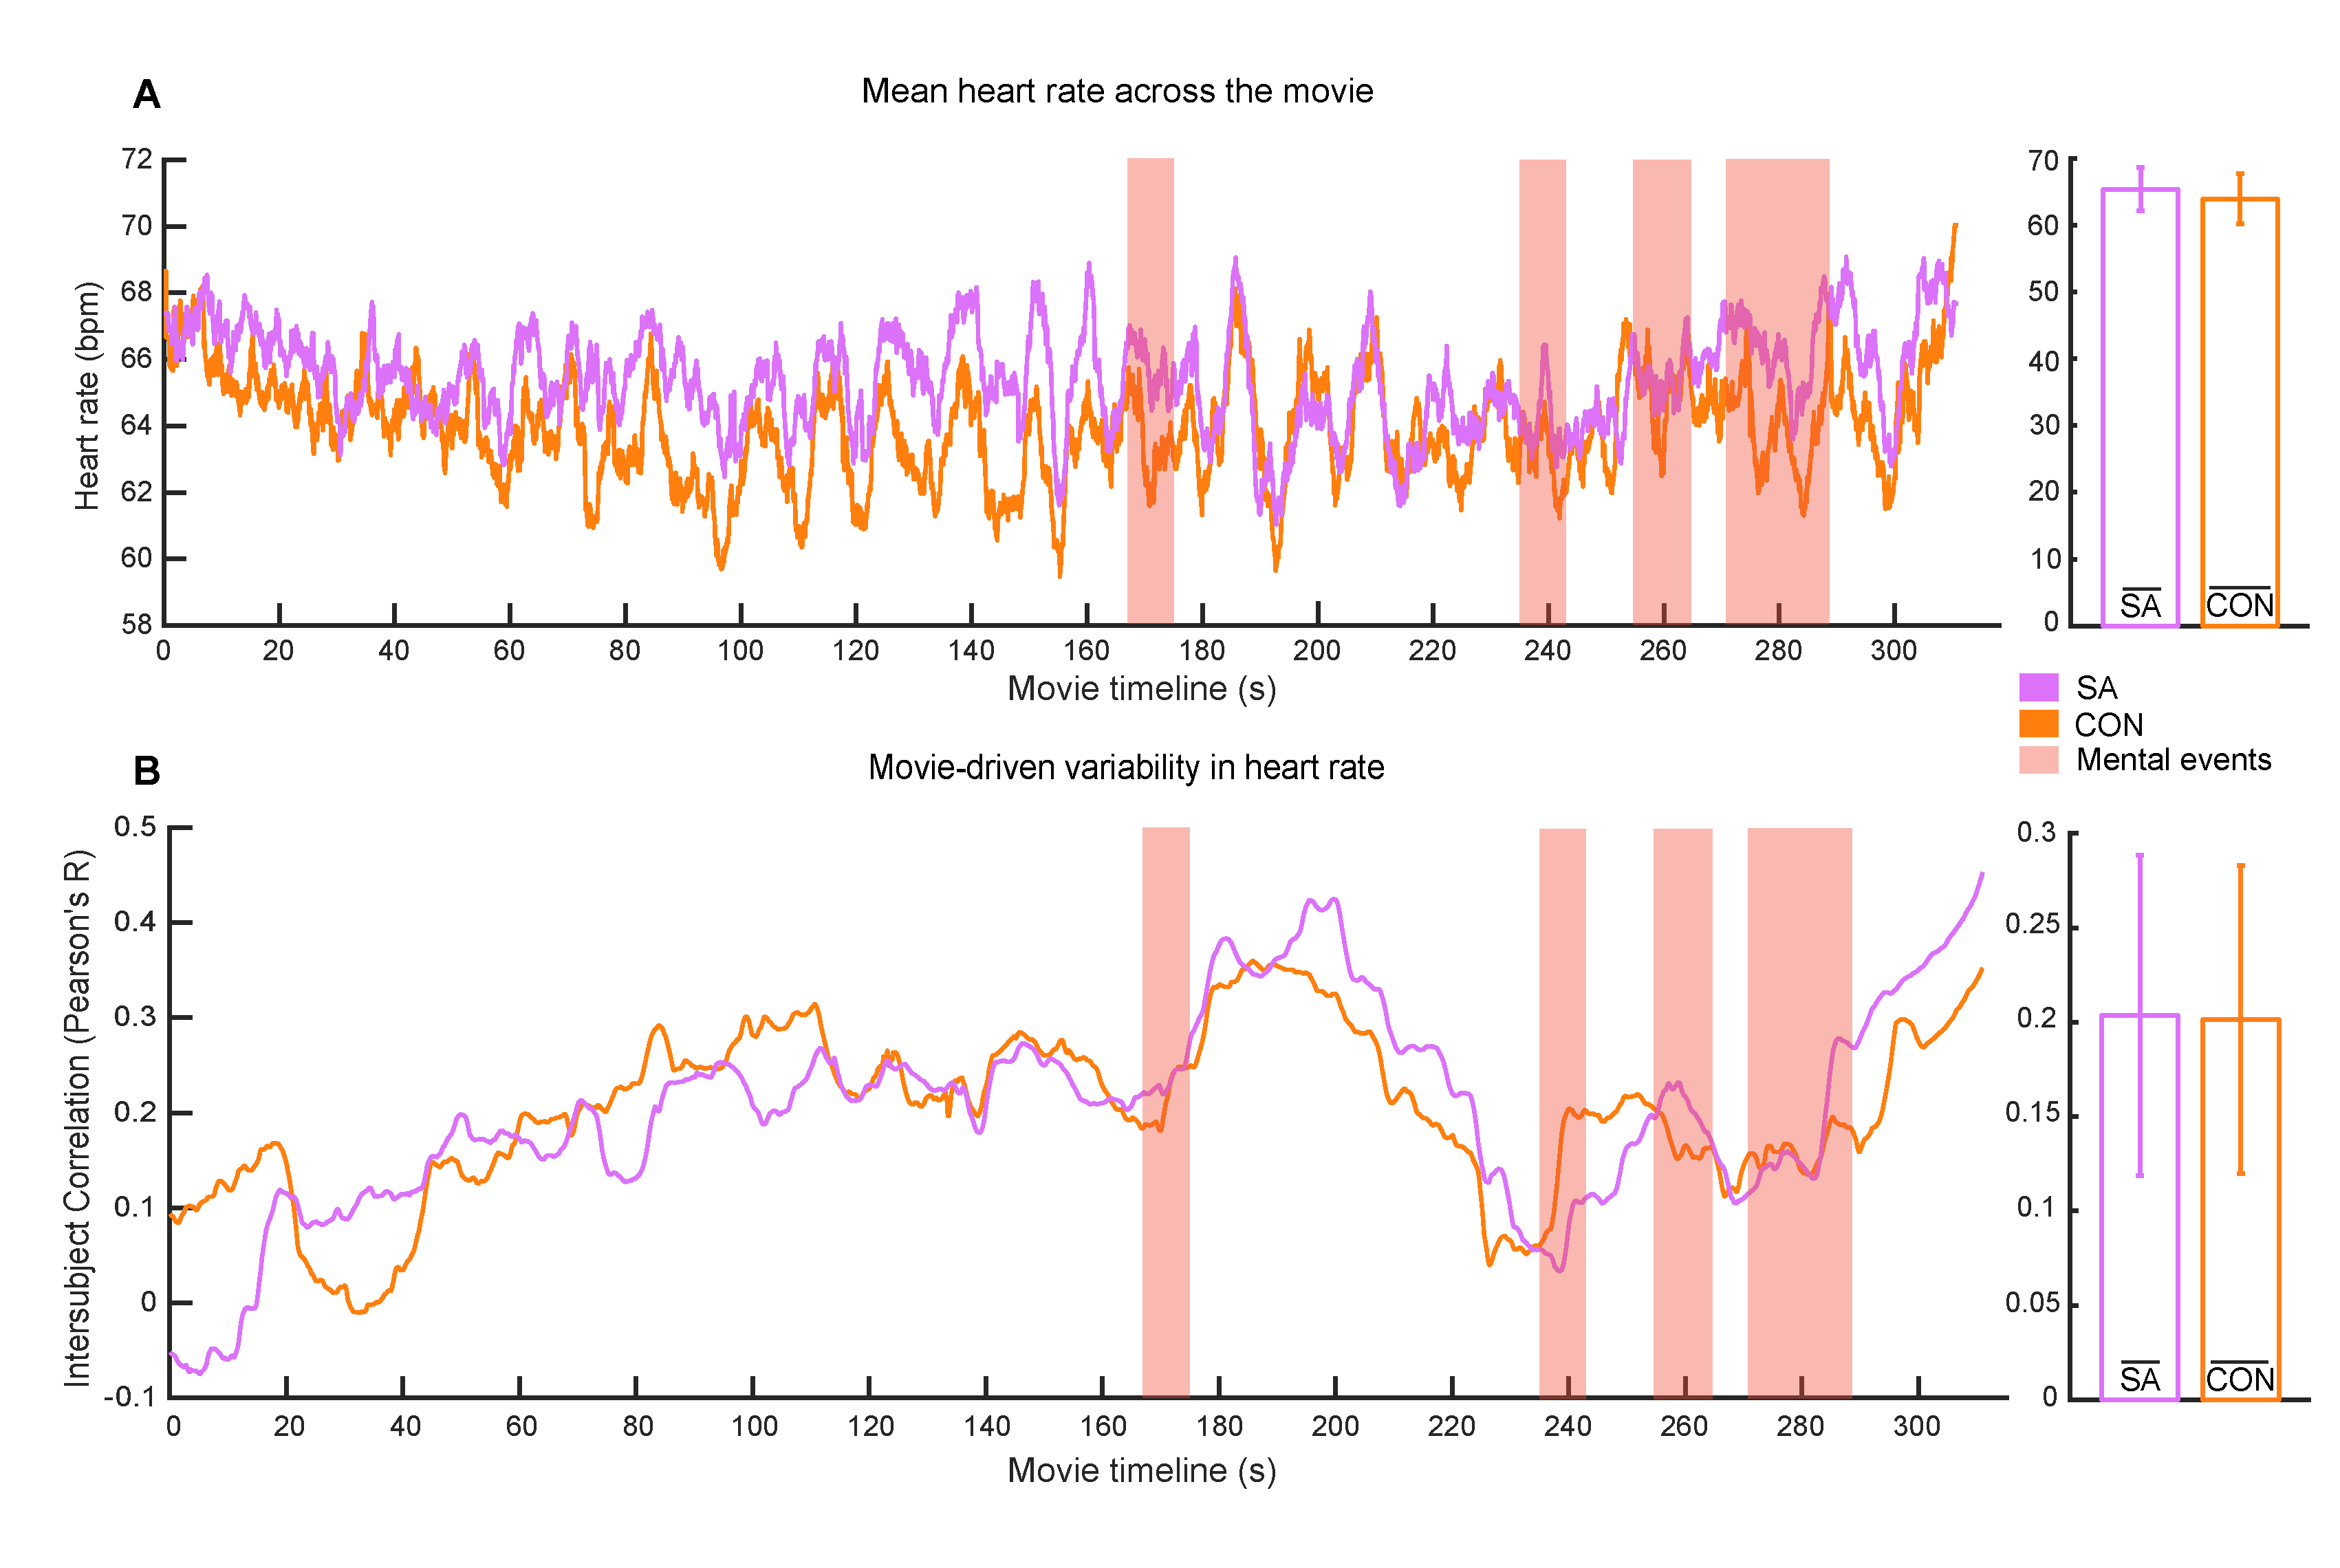
\includegraphics[width=1\textwidth]{./Chapters/03_MentalizingSA/Images/HeartRate.eps}}
	\caption{(a) Mean heart rate measured across the duration of the movie for both socially anxious and control participants. Adjacent histograms show the aggregated mean heart rate throughout the entire film for each group, with error bars representing 95\% confidence intervals. (b) Average intersubject correlation coefficients illustrate the intersubject variability in heart rate response during the movie among socially anxious and control participants. There were no significant differences detected in either metric between the two groups.}
    \vspace*{-10pt}
	\label{fig:heart-rate}
\end{figure}



\vspace{10pt}

\begin{figure}[!t]
	\centering
    \makebox[\textwidth][c]{\includegraphics[width=1\textwidth]{./Chapters/03_MentalizingSA/Images/ISCPupil.eps}}
	\caption{Dynamic intersubject correlation analysis revealed substantial fluctuations in variability throughout the film. Socially anxious participants exhibited lower correlations, indicative of higher variability in pupil responses compared to controls. Nonetheless, these differences did not reach statistical significance at any point during the viewing.}
    \vspace*{-10pt}
	\label{fig:isc-pupil-sa}
\end{figure}



%\afterpage{\blankpage}
\chapter[Oscillatory Language Dynamics in Autism]{As the Sentence Unfolds: Oscillatory Dynamics of Language Processing in Verbally Competent Autistic Adults}
\label{ch:language_asc}

\begin{center}
    \large\textit{Abstract}
\end{center} 

{\abstractfont 
Autistic individuals often experience challenges and delays in language development, yet it remains unclear whether their language processing unfolds differently from that of neurotypical individuals in adulthood. In this study, we used EEG to examine real-time oscillatory neural dynamics as autistic adults and verbally and age-matched neurotypical controls read both structured sentences and pseudoword lists. Comparing these two conditions in reading revealed systematic spatiotemporal power dynamics across theta, alpha, beta, and gamma frequency bands across participants. These patterns included high power in the beta band during sentence reading and a progressive intensification of this beta signature as sentences unfolded, indicating cumulative processing of linguistic structure. Importantly, these oscillatory patterns appeared consistent across both autistic and neurotypical participants, with current analyses revealing no statistically significant differences in spatiotemporal progression or lateralization between groups. These findings suggest that sentence-level linguistic processing unfolds neurophysiologically in a similar manner in verbally competent autistic adults, suggesting that other underlying factors may contribute to language developmental delays in autism. \par
} 

\vspace*{\fill} 

\thispagestyle{empty}

\newpage

\section{Introduction}

Delays in language development are a common feature of autism, with approximately one-third of individuals remaining minimally verbal throughout their lives \citep{apa2013,kim2014,velikonja2019}. Although not a diagnostic criterion, autism is often first recognized due to atypical or delayed patterns of speech development during the second year of life, when most children of the same age begin to establish vocabularies comprising numerous words \citep{short1988}. However, such delays in expressive language during early preschool years are not unique to autism, and some individuals with autism acquire language typically despite marked social deficits \citep{anderson2007}. These observations underscore the complexity of language development in autism, highlighting the need to investigate whether language processing is fundamentally different, potentially involving distinct neural mechanisms even in verbally competent adults, or whether other underlying factors are responsible for the observed delays in language acquisition.

In search of a possible biomarker of autism and the associated language difficulties, a multitude of studies have been performed on the neural underpinnings of language processing in autism. Reduced neural activation to language and auditory stimuli has been found in brain regions typically involved in language \citep[for reviews]{groen2008,philip2012}. These results, however, are not always consistent \citep{tryfon2018}. A crucial challenge in interpreting these findings is that most studies depend primarily on neuroimaging techniques like fMRI, which restricts our insight into the neurophysiological processes involved in linguistic comprehension in autistic individuals. 

Electrophysiological investigations into language processing can provide insights on the mechanisms involved and their time course. These mechanisms operate at different frequencies that reflect circuit-level functions. These electrophysiological studies, however, are scarce in the current literature. A pair of studies investigated this in neurotypical individuals by having participants read sentences or pseudoword lists in an RSVP (Rapid Serial Visual Presentation) paradigm and applying Electroencephalography (EEG) and Magnetoencephalography \citep[MEG;][]{bastiaansen2010,bastiaansen2015}. This sentences vs. pseudoword list contrast probes the word-by-word operation of building a sentence-level representation, known as linguistic structure building. Firstly, they showed that higher power in the beta band was elicited at sensors over central, frontal, and bilateral parietal brain areas in response to linguistic structure building, as well as higher power in the theta band at sensors over right parietal areas. In terms of the time course of these effects, both studies found increasingly large beta and theta power differences between structure building and non-structure building conditions over the course of the sentence. Increases in beta and alpha power during linguistic structure building are suggested to reflect the maintenance of the sentence-level representation \citep{engel2010,lewis2016}, while theta may be linked to keeping sequentially ordered information in working memory \citep{roux2014,vignali2016}. In the gamma band, intracranial findings showed a ramping increase in power across the sentence structure \citep{fedorenko2016}, possibly reflecting (visual) information held in working memory \citep{bastos2018,honkanen2015,roux2014,vignali2016}. Whether these neural mechanisms are different in autistic individuals, is still an open question.

A more common finding for the neural basis of language processing in autistic individuals is reduced left-lateralized activation, often a consequence of increased involvement of the right hemisphere during language processing \citep{herringshaw2016}. This phenomenon was observed in semantic processing \citep{knaus2008}, lexico-semantic processing \citep{coffeycorina2008}, phonological processing \citep{dawson1986}, and sentence processing \citep{muller1999}. A recent, relatively well-powered study on linguistic structure building found reduced left-lateralization in autistic individuals using a similar linguistic structure building contrast as in the Bastiaansen et al. studies \citep{jouravlev2020}. Given the fact that most of these studies on the lateralization of language processing used fMRI, it is an unresolved question whether differences in lateralization in autism have a temporal component, i.e., whether they occur early or late during linguistic structure building. This research on lateralization is of clinical relevance because lateralization during language processing and measures of language ability are uniquely correlated in autistic individuals \citep{lindell2013}. Thus, findings could provide clues regarding the cause of autism-specific language difficulties. 

Considering the replicated findings in the two studies by Bastiaansen et al., the beta power increases provide a useful neural marker of structure building across the sentence. This marker can consequently be used to examine and compare structure building between autistic and neurotypical individuals, in addition to the degree of lateralization of structure building. Therefore, our aim for this study was to investigate the oscillatory activity during linguistic structure building, in particular the beta band, in autistic and neurotypical individuals. To tap into this broad linguistic process, we used the sentences vs. pseudoword list contrast from \cite{jouravlev2020}. First, higher beta power for sentences (linguistic structure building) compared to pseudoword lists was expected based on the findings from previous studies using this contrast \citep{bastiaansen2010,bastiaansen2015}, and this difference was expected to increase as the sentences unfold. Again based on previous work, we predicted that these effects would be maximal at electrodes over parietal regions. Given the inconsistent findings, we had slight expectations for stronger beta power in autistic individuals, although this is based on findings using different techniques and contrasts \citep{philip2012}. A second aim of our study was to investigate the degree of left-lateralization of power, in particular the beta band as an index of linguistic structure building, and its progression over time. This left-lateralization was calculated to compare between autistic and neurotypical individuals. Since one of the key motivations for using EEG was to observe potential temporal dynamics related to degree of lateralization in autistic vs neurotypical individuals, the beta power lateralization was computed and compared across time in one-second windows. Afterwards, these lateralization  indices were compared separately at each of these time points between autistic and neurotypical groups, and compared on their rate of linear increase or decrease. We expected beta power to be more left-lateralized in neurotypicals compared to autistic individuals, following the fMRI literature showing differences between the two groups. Moreover, this difference in lateralization of beta power between groups may reasonably be expected to be larger at later time points after there has ostensibly been more time for structure building to take place. By analyzing these oscillatory dynamics, we seek to determine whether linguistic structure building is altered in autism, shedding light on its potential role as a source of communicative variability in autistic individuals.

\section{Materials and methods}

\subsection{Participants}
Forty autistic individuals (ASC) were included in this study on the basis of having a diagnosis of Autism Spectrum Disorder, as well as 36 neurotypical (NT) individuals. They were recruited from advertisements on social media, posters on campus, and Radboud University's participant database. They were included as autistic participants if they had an official diagnosis by a qualified clinician \citep{apa2013}, which was further validated by their scores on the Autism-Spectrum Quotient questionnaire \citep[AQ]{baron-cohen2001AQ}. The autistic participants can be classified as high-functioning given the low support demands in their daily lives. Exclusion criteria for all participants constituted severe cognitive impairment, systemic disease, a history of neurological impairment, and the use of psychotropic medication or systemic glucocorticoids. Each participant performed the experiment while EEG data was collected, after which the participants filled out a questionnaire with questions and tasks assessing a.o. their IQ, handedness, and autistic traits \citep{baron-cohen2001AQ,raven1989,veale2014}. Eight additional individuals participated in the study but their EEG data were not included in the study. The data of four of these participants were excluded due to technical malfunctions during the session. The other four participants' data were excluded due to poor data quality, for which less than 20 trials per condition were included after artifact rejection, or a full coverage of the head could not be established due to rejected bad electrodes. All participants gave written informed consent for the study protocol, which was approved by the local ethics committee (CMO region Arnhem-Nijmegen, file number 2019-6059). Participants were all compensated for their time investment and their travels.

The autistic and neurotypical individuals were matched on age, gender, handedness, and both verbal and non-verbal IQ (see Table~\ref{tab:ppt-stats-lang}). Statistical tests did not reveal differences between the autistic and neurotypical groups on gender balance (55.0\% vs. 44.4\% women, \textit{$\chi$\textsuperscript{2}} (1, \textit{N} = 76) = 0.48, \textit{p} = .49), on age (M \textpm{} SD 28.9 \textpm{} 6.8 vs. 27.0 \textpm{} 5.6, \textit{t}(74) = 1.29, \textit{p} = .20), on handedness (M \textpm{} SD 69.6 \textpm{} 69.8 vs. 84.7 \textpm{} 51.9, \textit{t}(74) = -1.15, \textit{p} = .25), or on verbal IQ measured by the Vocabulary and Similarities subscales of the Wechsler Adult Intelligence Scale \citep[128 \textpm{} 7 vs. 128 \textpm{} 16, \textit{t}(74) = -0.07, \textit{p} = .95]{wechsler1997} and performance IQ measured by the timed version of the Raven's Progressive Matrices test \citep[102 \textpm{} 9 vs. 103 \textpm{} 14, \textit{t}(74) = -0.35, \textit{p} = .73]{raven1989}. The Autism-Spectrum Quotient, as expected, showed a large difference between autistic and neurotypical participants (30 \textpm{} 9 vs. 14 \textpm{} 6, \textit{t}(74) = 9.23, \textit{p} <  .001), validating the distinction between the two groups.

\begin{table}[ht]
    \captionsetup{justification=raggedright, singlelinecheck=false, font = normal} % Left-align the caption
    \setlength{\tabcolsep}{7.5pt} % Adjust column spacing if needed
    \renewcommand{\arraystretch}{1.5} % Adjust row spacing
    \caption{Demographic data}
    \label{tab:ppt-stats-lang}
    \begin{tabular}{llll}
    \hline
    \textbf{} & \textit{ASC Group} & \textit{NT Group} & \textit{Group Difference} \\
    \hline
    N (women:men) & 40 (22:18) & 36 (16:20) & \textit{$\chi$\textsuperscript{2}}(1, N = 76) = 0.48, \textit{p} = .49 \\
    Age (years) & 28.9 (6.8) & 27.0 (5.6) & \textit{t}(74) = 1.29, \textit{p} = .20 \\
    Handedness (EHI) & 69.6 (69.8) & 84.7 (51.9) & \textit{t}(74) = -1.15, \textit{p} = .25 \\
    Verbal IQ (WAIS-III) & 128 (7) & 128 (16) & \textit{t}(74) = -0.07, \textit{p} = .95 \\
    Non-verbal IQ (RPM) & 102 (9) & 103 (14) & \textit{t}(74) = -0.35, \textit{p} = .73 \\
    Autism Quotient & 30 (9) & 14 (6) & \textit{t}(74) = 9.23, \textit{p} < .001 \\
    \hline
    \multicolumn{4}{l}{\footnotesize{Values are given as Mean (Standard Deviation). ASC, Autism Spectrum Condition; NT, Neurotypical.}} 
    \end{tabular}
\end{table}

\subsection{Experimental design}
Neural responses to linguistic structure building were assessed with a reading paradigm based on \cite{fedorenko2010}, contrasting two conditions: sentences and pseudoword lists. Sequences in both conditions contained twelve words or pseudowords, presented serially at a rapid pace. The sentences and pseudoword lists were matched in the number of letters and syllables (letters: M\textsubscript{SEN} (SD\textsubscript{SEN}) = 72.5 (5.8), M\textsubscript{LIST} (SD\textsubscript{LIST}) = 72.6 (6.2); syllables: M\textsubscript{SEN} (SD\textsubscript{SEN}) = 20.7 (2.1), M\textsubscript{LIST} (SD\textsubscript{LIST}) = 20.8 (2.2)) and the topics described in the sentences were varied. The pseudoword lists were created by replacing the content words in the sentences with pseudowords, and scrambling all (function) words and pseudowords in the sentence. Two independent native Dutch raters confirmed that the pseudowords did not resemble existing Dutch words. To ensure that participants were closely reading all sequences, they were given a memory task to answer whether a probe word was presented in the sequence they just read. All sequences were presented in a randomized order for each participant, and presented in blocks of three sequences for each condition. Before each block, a fixation cross was presented for a random duration between 4000 and 7750 milliseconds. Before each sequence, a fixation cross was presented for 200 milliseconds. Each word or pseudoword was presented for 400 milliseconds. After the sequence, the memory probe word of the task was presented for 750 milliseconds. These durations are specified for the experiment presentation software, but the screen refresh time is added to these durations. For a subset of the participants in this study, the screen refresh times were 33 ms longer due to changes following hardware replacement. Importantly, the proportion of participants with different screen refresh durations is exactly the same between groups (75\% longer and 25\% shorter durations for both groups), ruling out the possibility of this difference explaining group effects. This difference is further corrected for in the data analysis section (see section \ref{preprocessing}). 

\begin{table}[ht]
    \captionsetup{justification=raggedright, singlelinecheck=false, font = normal} % Left-align the caption
    \renewcommand{\arraystretch}{1.5} % Adjust row spacing
    \caption{Example sequences for the two conditions with English translation.}
    \label{tab:example_sequences}
    \small
    \begin{tabular}{lp{8.2cm}}
    \hline
    \textit{Condition} & \textit{Example item} \\
    \hline
    \small{SENT (sentence)} & \small{Meer dan duizend arbeiders werken in het moderne bedrijf tegenover het station.} \\
     & \small{\textit{More than a thousand employees work at the modern company across from the station.}} \\
    \small{LIST (pseudoword list)} & \small{van eingelzing bepen camzen parpisch uit naar groden kastren van naar moemels} \\
     & \small{\textit{from} eingelzing bepen camzen parpisch \textit{out to} groden kastren \textit{of to} moemels*} \\
    \hline
    \multicolumn{2}{l}{\footnotesize *Only translations for existing Dutch function words.} \\
    \end{tabular}
    \normalsize
\end{table}

\begin{figure}[!ht]
	\centering
    \makebox[\textwidth][c]{\includegraphics[width=1\textwidth]{./Chapters/04_LanguageASC/Images/ExpDesign.eps}}
	\caption{Schematic of the task performed by autistic and neurotypical participants during the EEG experiment to ensure a close reading of the sequences. Sentences (shown here) or pseudoword lists were presented by showing every word or pseudoword consecutively for 400 ms, preceded by a fixation cross for 200 ms. After each sequence, participants were asked whether a target word (here: \textit{station}), on screen for 750 ms, was shown in the sequence they had just read, which they indicated via button press.}
    \vspace*{-10pt}
	\label{fig:exp-design}
\end{figure}




\subsection{Procedure}
Measurements took place in an electrically-shielded, sound-proof room. Before the EEG preparation started, participants were informed about the steps of the EEG preparation and measurement procedures. They received instructions about the task, including having to answer whether the probe word was part of the sequence that was presented before. They were instructed to use their left index finger to press a left button for yes and their right index finger to press a right button for no. They were also informed that while the reading and task decision tempo was quite high, their response would still be registered if they pressed the button after the probe word disappeared from the screen. Lastly, they were instructed to minimize head movement as much as possible during the task. The participants rested their head on a head and chin rest, reducing head movement, with a viewing distance of 59 cm. The words and pseudowords in the sequences and fixation crosses were presented in black text in the center of the screen with a light grey background. All text was presented in the Courier New font with size 18. Both the target word and `yes' and `no' were presented in red text. The measurement lasted for 12 minutes. 

\subsection{EEG recordings}
A fitting 64-electrode actiCap with active sensors was placed on participants' heads. The left mastoid electrode was used as a reference and an electrode at the center of the forehead as a ground electrode. To measure vertical eye movements, two electrodes were placed at the supra- and suborbital ridges of the right eye. For horizontal eye movements, two electrodes were positioned in a right-to-left outer canthal bipolar montage. Electrode impedance was kept below 25 kilo-ohms during the experiment. EEG data were amplified and collected with BrainAmp DC amplifiers at a sampling rate of 5000 Hz with a 0.1 - 1000 Hz band-pass filter. 

\subsection{Behavioral analysis}
To check whether participants were sufficiently engaged in the experiment, response rate for the memory task was calculated for each participant. With an independent \textit{t}-test (\textit{alpha} = 0.05) we assessed whether autistic and neurotypical individuals responded to a similar number of trials. Reaction time and accuracy to the memory task was recorded in order to compare the difficulty of the task between conditions and groups. To capture the variability in performance across trials and subjects, generalized linear mixed effects models in R (version 4.3.3) were used to investigate reaction time and accuracy with the \textit{lme4} package \citep{bates2015}. For modelling reaction time, participant group (autistic or neurotypical) and condition (sentence or pseudoword list) were included as fixed effects with their interaction term, together with a subject-specific intercept as random effect. This reaction time model was created to assume an inverse gaussian distribution with a log link function, optimized to only fit positive data \citep{lo2015}. The same model structure of fixed and random effects, but with a binomial distribution and a logit link function, was used to calculate effects for accuracy. Significance of the effects was identified with the \textit{lmerTest} package \citep{kuznetsova2017}, which uses Satterthwaite's method to calculate \textit{p}-values.

\subsection{EEG Preprocessing} \label{preprocessing}
EEG data were analyzed using the Fieldtrip toolbox \citep{oostenveld2011} in a MATLAB environment (R2020a; Mathworks, Inc.). The data were processed with a low-pass filter at 199 Hz and a band-stop filter at 50, 100 and 150 Hz to reduce effects of power line noise (50 Hz). Artifact rejection was done in two stages of visual inspection of the data. First, the continuous EEG data were visually inspected for blinks, eye movements and high-frequency noise. Segments containing these artifacts were replaced with zeros. At trial definition, trials with less than two seconds of included data were excluded from further analyses. Afterwards, trials and channels containing noise and artifacts were rejected from the data on the basis of amplitude variance and kurtosis (all measured per trial across time). All scalp electrodes were re-referenced to the common average reference. Bad channels were repaired by reconstructing them from the average of their neighbouring channels. After artifact rejection, 19\% of all trials were excluded. Importantly, the number of rejected trials was comparable for the two conditions (M\textsubscript{SEN} = 19.2\%, M\textsubscript{LIST} = 17.8\%, \textit{t} (75) = 1.36, \textit{p} = .18) and the autistic and neurotypical groups (M\textsubscript{ASC} = 18.4\%, M\textsubscript{LIST} = 18.6\%, \textit{t} (75) = -0.09, \textit{p} = .93). Finally, all data were segmented from -300 ms to 5500 ms relative to the onset of the first word in the sequence. This trial duration was chosen as it corresponds to the shortest trial across all participants. Because of this procedure, the analysis excludes the last 396 ms of longer trial durations that are due to longer screen refresh times (12 (pseudo)words * 33 ms of screen refresh duration = 396 ms). This procedure was done to be able to include data from participants with both shorter and longer screen refresh times. Crucially, power changes in the sentence vs. pseudoword list contrast were not different for participants with short or long screen refresh times (see Supplementary Note \ref{suppl-note}).

\subsection{Sentences vs. pseudoword lists power and statistical analysis}
Time-frequency spectra were calculated for each trial separately using a sliding-window approach with a Hanning taper and the application of a fast Fourier transform. Frequencies were estimated between 2 and 100 Hz in steps of 2 Hz with a sliding window of 500 ms applied in steps of 20 ms. The sliding window length was chosen in order to optimize sensitivity in the beta band, the frequency band of interest, which tends to be relatively short-lived \citep{jones2016}. This means that the power in every time-frequency point represents a weighted average of -250 ms to 250 ms at the specified timepoint. Power values were then expressed as a relative change from the standard deviation of the power of all trials. This \textit{z}-scoring was done over all trials of both conditions within the full time window. This was performed separately for each channel, frequency, and time bin and resultant \textit{z}-scored power values were then averaged across trials. 

To calculate and compare power changes between the sentence and pseudoword list conditions, statistical testing was performed with cluster-based random permutation testing on power changes in the two conditions averaged over trials \citep{maris2007}. This method was chosen because it elegantly handles the multiple comparisons problem. Briefly summarized, for every data point (electrode-frequency-time point) a dependent \textit{t}-test is performed which generates uncorrected \textit{p}-values. These are compared against a pre-set significance level (here, 5\% two-tailed) and data points at which \textit{p}-values fall above this level are discarded. The remaining data is used to form clusters based on their adjacency in space (channels), frequency, and time. Cluster-level statistics are then computed by summing the \textit{t}-values of the data points that make up each cluster. Next, a permutation distribution is created by randomly assigning participant averages to one of the two conditions, an approach that is repeated 5000 times. Each permutation, cluster-level statistics are calculated, with the highest cluster-level statistic included in the permutation distribution. The cluster statistic for the measured data was compared against this distribution, and clusters that fell in the lowest or highest 2.5\% of the distribution were considered statistically significant. Statistical testing was first performed over the full frequency range between 2 and 100 Hz, allowing both spatial and spectral clustering for multiple comparison correction. Afterwards, the effects were separately tested in theta (3 - 7 Hz), alpha (7 - 13 Hz), beta (14 - 20 Hz) and gamma (60 - 80 Hz), averaged over the specific frequency band. The time window for which we tested the data was from 0 to 5200 ms relative to the onset of the first word of the sequences. Reported effect sizes for the cluster on the basis of which the H0 was rejected, were calculated by averaging over the data in this cluster. 

For a between-group comparison of power changes during linguistic structure building, the power difference between the sentence and pseudoword lists was calculated by subtracting the grand averages of the pseudoword lists condition from the sentences condition for each subject. Power changes were then compared between autistic and neurotypical individuals with cluster-based permutation testing using independent \textit{t}-tests (\textit{alpha} = 0.05). Bayes Factors were computed for between-group differences in power changes in peak channels and timepoints to assess the evidence for the null model and the model that specifies group.

To more sensitively assess whether this contrast, ostensibly designed to probe linguistic structure building, is constant or changes over time, a second test was performed.  For this test, a linear regression model across trial time course was fit to the power for each subject, condition and frequency band at its peak channel. These subject-specific regression fits were then compared between autistic and neurotypical individuals and sentence and pseudoword list conditions in an ANOVA with group, condition and their interaction as independent variables. 

\subsection{Laterality index}

For comparing lateralization of the linguistic structure building effect in the brain between groups and its progression over time, the previously calculated power values were split into five time windows of one second, spanning the trial time course, and averaged over these windows and over each of the four frequency bands. For these frequency bands and the five time windows, the difference in power between the sentence and pseudoword list conditions was calculated as the normalized power difference as the following: (SENT - LIST) / (SENT + LIST). This normalization was done to take into account electrodes that have differing levels of signal strength or quality. A laterality index for these power differences was calculated for all non-midline electrodes by subtracting the power of the right electrode from the power of the left electrode (Left - Right). This resulted in values representing the extent of the left-lateralization of the power difference for each electrode pair. While lateralization is more commonly calculated by dividing this Left-Right electrode difference by the sum of these two power values, this would lead to extreme values due to possible negative and positive values in the denominator. For this reason, we chose to exclude the denominator from the calculation. Note that these values represented the effects picked up on the scalp and not the precise location of the underlying neural generators due to volume conduction.

Grand averages of the laterality index were computed for each frequency band across time. To determine whether time-frequency power in the four frequency bands was lateralized in the first place, the laterality indices were compared to zero with the aforementioned cluster-based permutation method using dependent \textit{t}-tests (\textit{alpha} = 0.05). This was done for the autistic and neurotypical group separately. Crucially, the lateralization of power during linguistic structure building were then compared between the autistic and neurotypical participant groups with a cluster-based permutation method using independent \textit{t}-tests (\textit{alpha} = 0.05). This comparison of lateralization index between groups was chosen because it mirrors the approach of the fMRI study which found group differences in lateralization of the sentences vs. pseudoword lists contrast \citep{jouravlev2020}. The beta band was of particular interest in this analysis on account of previous studies showing it is the strongest index of linguistic structure building \citep{bastiaansen2010,bastiaansen2015}. 

To additionally assess group differences in language laterality more sensitively, we identified four electrodes where the sentence vs. pseudoword list contrast from the previous analysis was strongest across groups. These electrodes were therefore identified independently of the whole-brain laterality analysis. In these four peak electrodes, the average laterality index was calculated for each frequency band and time window. To determine whether power during linguistic structure building was lateralized in the first place, these average laterality indices were first compared against zero in both groups. This comparison was done with dependent \textit{t}-tests Bonferroni-corrected for the number of time windows (\textit{alpha} = 0.01). Afterwards, the laterality indices were compared between autistic and neurotypical participants with an independent \textit{t}-test (\textit{alpha} = 0.01), and Bayes Factors were computed and reported to assess the evidence for the null model or the model that specifies group status.

Finally, to statistically evaluate the time course of the laterality, a subject-specific linear regression model was fit to the laterality indices, mirroring the procedure for the power values. These regression fits were first compared against zero to determine whether lateralization in the four frequency bands varied over time. To investigate the difference in laterality time course for autistic and neurotypical individuals, the subject-specific regression fits on laterality values were subsequently compared in an independent \textit{t}-test (\textit{alpha} = 0.05). 

\section{Results}
\subsection{Behavioral task}
When asked if a word or pseudoword was part of a sentence or a list they read, responses were logged for 95.2\% of the trials on average (SD = 10.4\%), meaning participants did not respond to 4.8\% of the trials or responded too late. In addition, no participants responded to less than 50\% of trials and most participants (60\%) responding to all or all but one of the trials. These results indicate that participants attended to the task at hand. Response rates were within the same range for autistic and neurotypical individuals (M\textsubscript{ASC} = 94.2\%,  M\textsubscript{NT} = 96.5\%; \textit{t} (74) = -0.97, \textit{p} = .33), showing that the participant groups are similarly engaged with the task. In terms of analyzing response performance, we found that 82.5\% of trials were answered correctly on average (SD = 12.2\%). Much higher accuracy was found for responses for sentences than for pseudowords (M\textsubscript{SEN} = 89.8\%,  M\textsubscript{LIST} = 75.2\%; beta = 1.62, SE = 0.12, \textit{z} = 13.2, \textit{p} <  .001). A similar pattern was apparent for reaction times: participants took an average of 706 ms to respond (SD = 112.9 ms), but were much faster when responding to sentences than to pseudoword lists (M\textsubscript{SEN} = 657.9 ms,  M\textsubscript{LIST} = 754.1 ms; beta =  -0.13, SE = 0.01, \textit{t} = -17.7, \textit{p} <  .001). When comparing response measures between groups, we see that autistic and neurotypical individuals were equally accurate in task performance  (M\textsubscript{ASC} = 82.5\%,  M\textsubscript{NT} = 82.5\%; beta = -0.11, SE = 0.17, \textit{z} =-0.68, \textit{p} = .50). Yet, autistic people were overall slower to respond than neurotypical participants (M\textsubscript{ASC} = 733.8 ms,  M\textsubscript{NT} = 675.1 ms; beta = 0.09, SE = 0.04, \textit{t} = 2.07, \textit{p} = .038). No interaction between participant group and task condition was found either for accuracy (beta = -0.27, SE = 0.17, \textit{t} = -1.61, \textit{p} = .11) or reaction time (beta = -0.01, SE = 0.01, \textit{t} = -0.52, \textit{p} = .61), which suggests that autistic participants show an equally large linguistic task effect as neurotypical individuals.


\subsection{Time Frequency Analysis}
\subsubsection{Sentences vs. pseudoword lists across and between groups}
Cluster-based permutation analyses showed that time-frequency power when reading sentences was significantly higher than when reading pseudoword lists in the full frequency range from 2 to 100 Hz (\textit{p} <  .001, \textit{d} = 1.33). The difference in power was present in all channels and time points up to 46 Hz (see Fig~\ref{fig:tf-spectrum-full}a). Analyses focused on the four frequency bands individually confirmed this difference between conditions for the beta (\textit{p} <  .001, \textit{d} = 1.81), alpha (\textit{p} <  .001, \textit{d} = 2.99), theta (\textit{p} <  .001, \textit{d} = 2.27) and gamma (\textit{p} = .03, \textit{d} = 0.42) bands.

\begin{figure}[!ht]
	\centering
    \makebox[\textwidth][c]{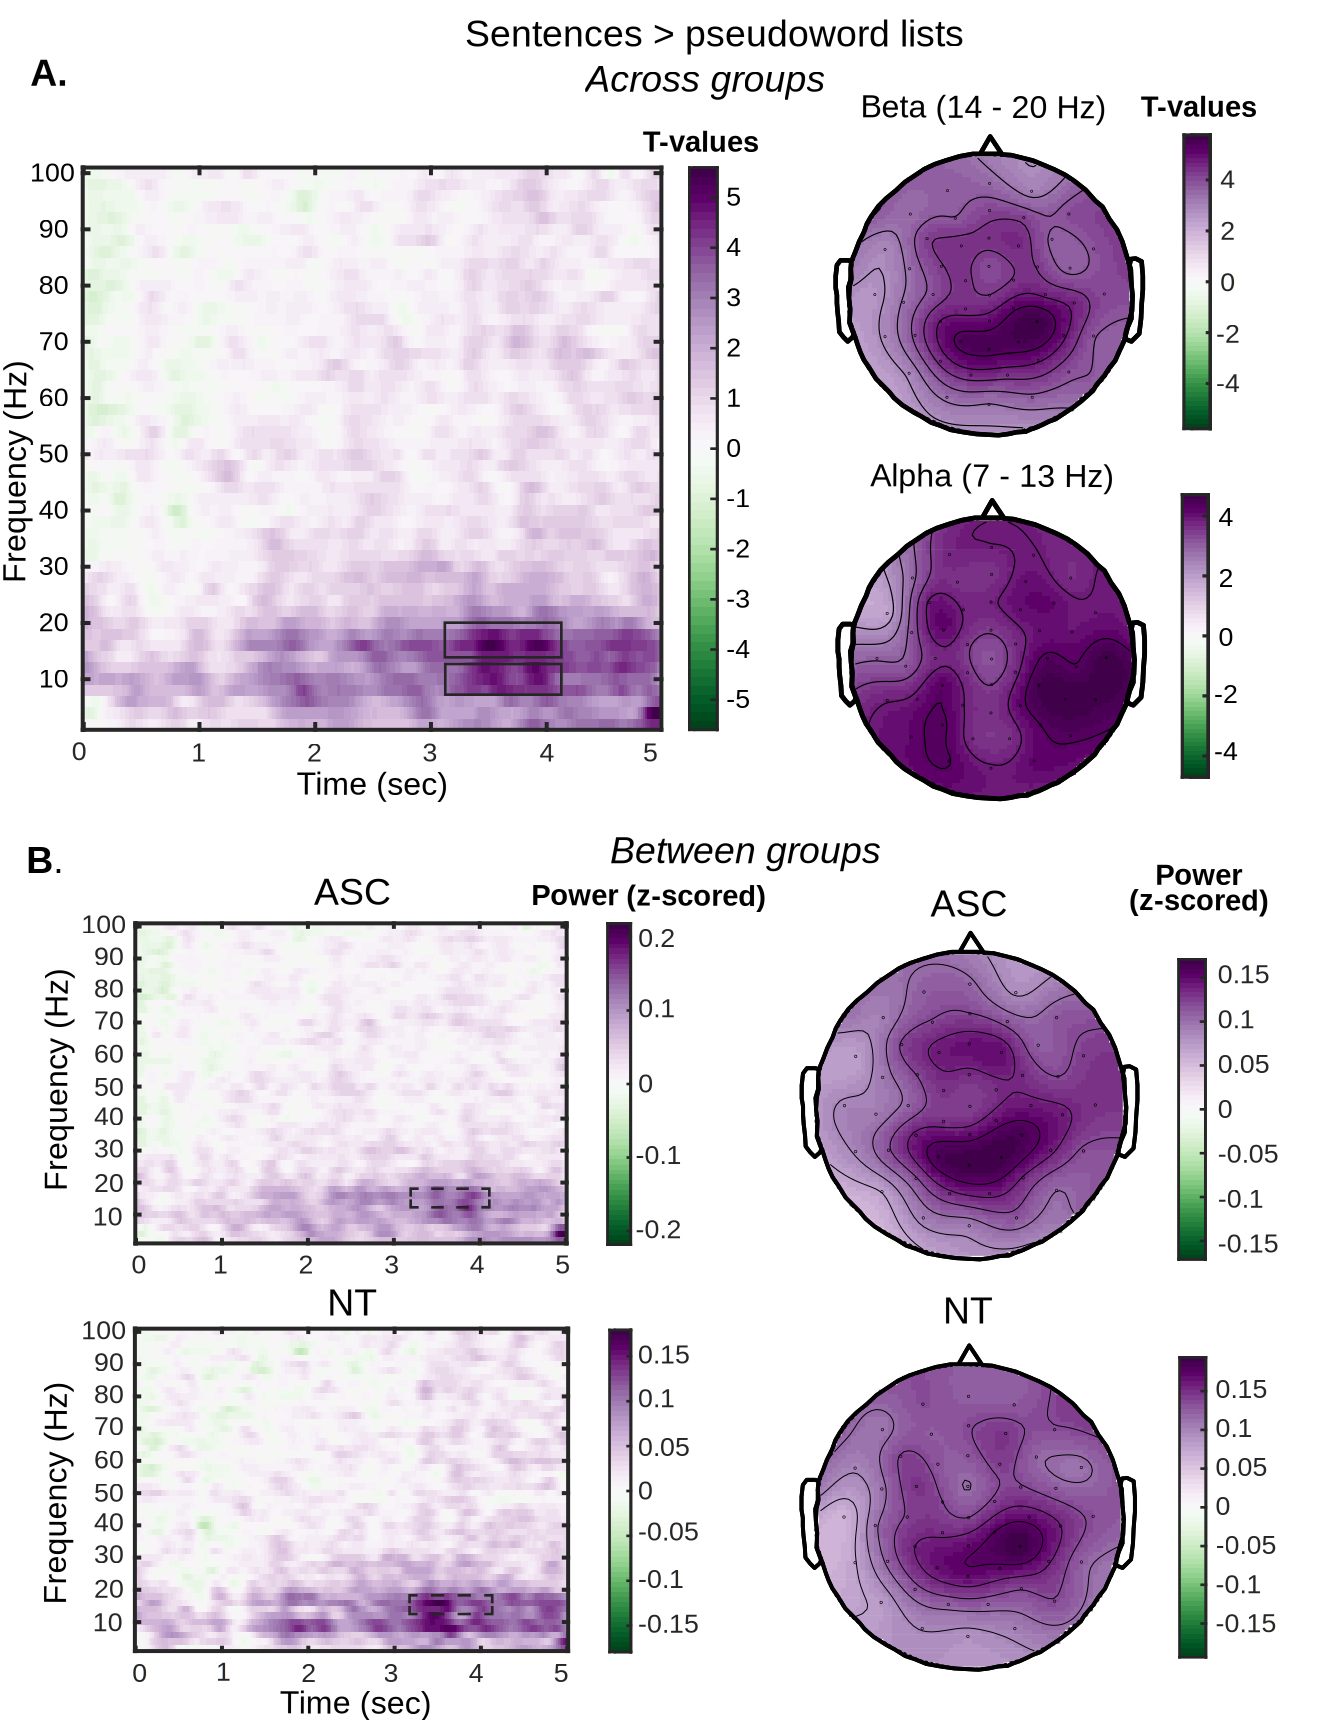
\includegraphics[width=.8\textwidth]{./Chapters/04_LanguageASC/Images/TFSpectrumFull_vert.eps}}
	\caption{Time-frequency (TF) dynamics in Sentences vs. pseudoword list contrast. (a) TF power is significantly different for the contrast, with power differences present across almost all channels, frequencies and timepoints. The color scale shows the relative difference in TF power (0 = no change). The timepoints and frequencies where the effect is strongest are indicated with boxes on the left, and the corresponding topography on the right for two different frequency bands: 14 - 20 Hz (beta) with bilateral posterior peaks, and 7 - 13 Hz (alpha) with a more widespread spatial effect. (b) TF power for the contrast was not different between neurotypical (NT) and autistic (ASC) participants. On the left, the similar TF spectra are shown, with the rectangle indicating the strongest power changes and on the right, the topography of this effect. }
    \vspace*{-10pt}
	\label{fig:tf-spectrum-full}
\end{figure}




The temporal dynamics of time-frequency power showed different patterns for the four frequency bands (see Fig~\ref{fig:tf-dynamics-topo}). The strongest power differences occurred in the latter part of the trial, peaking between 3 and 4 seconds after the onset of the first word, and in the beta band (around 16 Hz). This beta effect was primarily found at bilateral central posterior electrodes, peaking in the right hemisphere. Large power differences were also found for the alpha band (between 7 and 13 Hz), with a widespread spatial topography and strong effects at right parietal and left posterior electrodes. Given our experimental contrast, these alpha and beta differences likely contribute, at least partially and perhaps independently, to the cognitive process of linguistic structure building. 

\begin{figure}[!ht]
	\centering
    \makebox[\textwidth][c]{\includegraphics[width=1\textwidth]{./Chapters/04_LanguageASC/Images/TFDynamicsTopo.eps}}
	\caption{Time-frequency (TF) dynamics in Sentences vs. pseudoword list contrast across time and all participants for the theta (3 - 7 Hz), alpha (7 - 13 Hz), beta (14 - 20 Hz) and gamma (60 - 80 Hz) band.}
    \vspace*{-10pt}
	\label{fig:tf-dynamics-topo}
\end{figure}




Time-frequency power for this structure-building contrast was not significantly different between neurotypical and autistic individuals. The similar power spectra can be observed on the left hand side in Fig~\ref{fig:tf-spectrum-full}b, along with the topography of the strongest effect that was present in both groups. The similar time course of the two groups for both conditions can be seen in Fig~\ref{fig:tf-dynamics-peak}. A Bayesian analysis on the channels and timepoints showing maximal effects confirmed this lack of between-group differences for the beta (BF\textsubscript{NULL} = 3.31), alpha (BF\textsubscript{NULL} = 2.24), theta (BF\textsubscript{NULL} = 2.97) and gamma (BF\textsubscript{NULL} = 3.92) frequency bands. This indicates that oscillatory power in theta, alpha, beta, and gamma frequency bands during linguistic structure building are not different between neurotypical and autistic individuals. 

Subject-specific regression analyses indicated that progression of TF power over time was more positive while reading sentences compared to pseudoword lists in theta (\textit{d} = 0.48, \textit{p} = .004), alpha (\textit{d} = 0.46, \textit{p} = .005), and beta (\textit{d} = 0.96, \textit{p} <  .001; see Fig~\ref{fig:tf-dynamics-peak}a). This can be observed as the increasing difference in power over time between the conditions (see Fig~\ref{fig:tf-dynamics-peak}b). No significant difference between the condition in change over time was found for the gamma band (\textit{p} = .78). Time-frequency power change over time did not significantly differ for autistic and neurotypical participants in any of the four frequency bands, nor was there a significant interaction with condition. 

\begin{figure}[!ht]
    \vspace{10pt}
	\centering
    \makebox[\textwidth][c]{\includegraphics[width=.95\textwidth]{./Chapters/04_LanguageASC/Images/TFDynamicsPeak.eps}}
	\caption{Time-frequency (TF) power in the sentences and pseudoword lists (a) and difference of TF power between sentence and pseudoword list (b) across the trial time course for both groups. Power values are shown for the peak electrode in the sentences vs. pseudoword list contrast of the frequency band, of which the location is shown with scalp topography. Power differences over time between the two conditions were detected in the theta, alpha and beta band. No significant changes of TF power over time were found between autistic and neurotypical for any frequency band. Error bars indicate standard error. SENT = Sentences, LIST = Pseudoword lists. ** = \textit{p} < .001, * = \textit{p} < .01}
    \vspace*{-10pt}
	\label{fig:tf-dynamics-peak}
\end{figure}




\subsubsection{Lateralization of linguistic structure building}
Whole-scalp comparisons (all non-midline electrodes) were performed using cluster-based permutation statistics on the laterality indices of the sentences vs. pseudoword list contrast for the averaged one-second time windows and for the theta, alpha, beta, and gamma bands. Comparisons against zero in each participant group showed lower left-lateralization of power in the alpha band in the autistic individuals (\textit{p} = .002; see Fig~\ref{fig:laterality-topo}), driven by a cluster of frontal, lateral electrodes. No lateralized power was found in other frequency bands, nor in the neurotypical group. Despite this lateralization pattern in alpha, no differences in lateralization were found between autistic and neurotypical individuals in whole-brain comparisons for any of the four frequency bands. The similar lateralization patterns are shown across time in Fig~\ref{fig:laterality-dynamics-wholehem}.

\begin{figure}[!ht]
	\centering
    \makebox[\textwidth][c]{\includegraphics[width=1\textwidth]{./Chapters/04_LanguageASC/Images/LateralityTopo.eps}}
	\caption{Lateralization of time-frequency power in the sentences vs. pseudoword lists contrast detected across the hemisphere. Comparisons against zero showed significantly lower lateralization for autistic participants in the alpha band, driven by lateral electrodes. No significant changes of lateralization found between autistic and neurotypical for any frequency band. ** = \textit{p} < .01}
    \vspace*{5pt}
	\label{fig:laterality-topo}
\end{figure}




\vspace{.5cm}

\begin{figure}[!ht]
	\centering
    \makebox[\textwidth][c]{\includegraphics[width=.95\textwidth]{./Chapters/04_LanguageASC/Images/LateralityDynamicsWholeHem.eps}}
	\caption{Lateralization across the trial time course of time-frequency power in the sentences vs. pseudoword lists contrast for both groups averaged over the whole hemisphere. No significant changes of lateralization over time were found between autistic and neurotypical for any frequency band. Error bars indicate standard error. }
    \vspace*{-10pt}
	\label{fig:laterality-dynamics-wholehem}
\end{figure}


 

With a more spatially sensitive test, we inspected the topographies of the effects for the theta, alpha, beta, and gamma bands in the sentences vs. pseudoword list contrast, determined which electrodes showed maximal effects, and tested the laterality index between groups for these peak channels at each timepoint. For the beta, theta, and gamma band, independent \textit{t}-tests showed no statistically significant between-group differences in lateralization of the contrast at the selected electrodes in either of the five time windows (see Fig~\ref{fig:laterality-dynamics-peak}). This absence of group differences was corroborated by all Bayes factors for the null model being higher than for the model specifying group status (beta: BF\textsubscript{NULL} = 1.88 - 4.20, gamma: BF\textsubscript{NULL} = 2.63 - 4.13, theta: BF\textsubscript{NULL} = 1.82 - 4.13). For the alpha band, no significant between-group differences were found for four out of five timepoints (BF\textsubscript{NULL} = 2.39 - 4.19). There is evidence for a between-group difference in the alpha band between 1 and 2 seconds (BF\textsubscript{Group} = 1.4), although this difference did not pass the Bonferroni-corrected significance threshold (\textit{alpha}  = 0.01). These findings suggest that all frequency bands do not exhibit significant differential lateralization between neurotypical and autistic individuals during the process of linguistic structure building. 

After fitting a subject-specific linear regression model to the time course of lateralization during the sentence and pseudoword list conditions in the four peak channels, lateralization during linguistic structure building appeared stable across the trial, showing no deviating regression from zero (see Fig~\ref{fig:laterality-dynamics-peak}). Furthermore, lateralization was similarly stable for autistic and neurotypical individuals as no differences in time courses were found between the two groups. 

The analyses so far have regarded autistic and neurotypical individuals as separate categories, when autism can also be considered as a dimensional trait in the general population. To capture any lateralization effects beyond the case-control distinction of autistic and neurotypical individuals, we calculated Pearson's correlation between autistic trait strength and the sentences vs. pseudoword list contrast laterality indices for each time point at the four selected electrodes where the contrast was maximal in the analyses prior to computing the laterality index. Autistic trait strength was measured with participants' responses to the Autism-Spectrum Quotient questionnaire \citep[AQ;][]{baron-cohen2001AQ}. No statistically significant correlation was found for any of the four frequency bands. This corroborates the null finding in the case-control analysis that autism or autistic traits are not associated with lateralization differences during linguistic structure building. 

\section{Discussion}
While evidence on neurophysiological correlates of linguistic structure building during sentence reading in neurotypical individuals is growing, it remains unclear whether these are similar for autistic individuals. For this reason, we investigated how neural oscillations in autistic and neurotypical individuals are associated with linguistic structure building. Using a sentences vs. pseudoword list contrast, we replicated previous work showing that frequency-specific power associated with a sentences vs. pseudoword list reading contrast reaches maxima in the beta band (14 - 20 Hz) over bilateral parietal electrodes. The current study extended these findings with the novel result that this oscillatory activity during linguistic structure building is similar for neurotypical and autistic participants across theta, alpha, beta and gamma bands. We also observed larger differences over time during linguistic structure building in power in the beta, alpha, and theta bands but not the gamma band when comparing the regression fits over the course of the sequences. Furthermore, we showed that the degree of lateralization of power changes in the beta, alpha, theta and gamma bands associated with linguistic structure building was similar for neurotypical and autistic individuals. The degree of lateralization was similar at any time point in the sequence, and this stable degree of lateralization over time was present and similar in both groups. Crucially, taken together, these findings corroborate previous studies investigating frequency-specific beta power linked to structure building. In addition, the findings demonstrate that these beta effects, in addition to theta, alpha and gamma effects, are no different in autistic individuals. Moreover, they contradict fMRI findings \citep{jouravlev2020} showing differential lateralization in BOLD related to structure building between autistic and neurotypical individuals.

The peak effects of the linguistic structure building contrast were detected over bilateral parietal electrodes in the low-beta band, which is consistent with the location of large effects in earlier studies \citep{bastiaansen2010,bastiaansen2015}. Power in the beta band, in addition to the other frequency bands, was similar in our study for autistic and neurotypical individuals in this contrast. This deviates from findings in two fMRI studies who find lower activation for autistic individuals in left middle temporal gyrus during listening to sentences compared to rest \citep{muller1999}, and lower left inferior frontal activation but higher superior temporal activation when listening to sentences with the task to identify the agent or the patient in active or passive sentences \citep{just2004}. Notably, these fMRI contrasts and sentence processing tasks differ substantially from those of the current study, as well as the neuroimaging methods themselves. Since fMRI and EEG are not likely to capture the same exact neural signature, findings in one method are not expected to be identical to findings in the other method. Instead, they are complementary in capturing the underlying cognitive phenomenon.

The functional role of the beta power during linguistic structure building has previously been suggested to reflect syntactic unification, i.e., putting incoming words of a sentence together in a structure manner according to grammatical principles of the language to form a multi-word utterance \citep{bastiaansen2010,bastiaansen2015}. However, beta power has also been shown to decrease when syntactic unification becomes more demanding \citep{lewis2023}. Together with studies showing that beta power is also sensitive to other types of linguistic information during sentence comprehension (e.g., semantic and intonational anomalies), a more likely explanation might be that beta power supports the maintenance of a sentence-level representation during linguistic structure building \citep{lewis2016}. The maintenance role for the beta band in sentence comprehension is consistent with its role for other modalities such as motor control and visual attention \citep{engel2010}. This maintenance would be supported by increased top-down processing due to more prediction while processing a stimulus. This has been previously observed during visual attention and categorization tasks as increased beta power due to more top-down processing \citep{limanowski2020,antzoulatos2016}. These findings are consistent with our study, in which increased beta was observed for in the sentence reading condition. In this condition, a sentence-level representation could be formed, maintained and predicted for, which was not possible when reading pseudoword lists. 

While power in the gamma band is higher across sentences than pseudoword lists, we do not observe a power increase across the time course of the sequences when contrasting the two conditions. This finding differs from the results of an intracranial EEG experiment showing a ramping increase of beta power in a similar contrast over frontal and temporal electrodes \citep{fedorenko2016}. One potential explanation for this discrepancy is the difference in electrophysiological methods: it is possible that we did not pick up this ramping gamma effect due to the smearing of the signal from the volume conduction present in scalp EEG. Another possibility is that microsaccadic artifacts obscured a possible frontal effect in the current data, since those were not explicitly corrected for.   

A critical observation of the sentences vs. pseudoword list contrast that we used would be that it is a broad contrast which can capture a host of linguistic processes, not all of them related to structure building. The two conditions indeed differ in several respects, including lexical-semantics, syntactic structure, and situation model building. Yet, evidence that this contrast captures some linguistic structure comes from an ECoG study, in which the cognitive operation of merging words into multi-word phrases was probed with the same contrast \citep{nelson2017}. The authors successfully detected this `merge' operation, showing that the neural signal does not simply reflect the linearly increasing number of words, but responds to the demands of the syntactic tree-like structure of the sentence. Nonetheless, the primary goal of our study was not to probe the specificity of  the linguistic structure building captured by this contrast. We merely replicated existing findings linking this contrast to EEG, and investigated whether the neural marker of the process of interest is different for autistic and neurotypical individuals. 

In the current study, no lateralization differences were found in any frequency bands between autistic and neurotypical individuals, contradicting the fMRI literature. Additionally, there was an absence of lateralization in the neurotypical group for the alpha, beta and gamma band. This is in contrast with consistently reported left-lateralization of the BOLD signal in neurotypical individuals during language tasks \citep{fedorenko2010,pallier2011}. There are several ways in which the BOLD signal can translate to EEG frequency bands. First, gamma band power is known to show correlations with the BOLD signal \citep{scheeringa2016}. In our data, however, any left-lateralized gamma power we may have detected, was potentially obscured by microsaccadic activity. Left-lateralized BOLD signal is potentially also detectable as right-lateralized alpha and beta power in the EEG data given the anticorrelation of these frequency bands and the BOLD signal \citep{scheeringa2016}. Yet, we did not detect this in the data and instead, we picked up a different, non-lateralized source of neural activity. A possible candidate for this source may be the activity in the parietal and occipital lobes as seen in fMRI literature, since these areas also respond to the sentences vs. pseudoword contrast, albeit less intensely than fronto-temporal areas \citep{fedorenko2010}. More importantly, these areas are excluded from the parcel-constrained fMRI analysis in \cite{jouravlev2020}, who find left-lateralization present across participant groups and reduced in autistic participants. This means our data may have picked up on neural activity which was precluded to appear in \cite{jouravlev2020}. In addition, as previously mentioned, fMRI and EEG do not capture the same exact neural signature. Therefore, the strongest frequencies detected in the current EEG study, the alpha and beta band, may originate from a non-lateralized parietal or occipital source and may have obscured the left-lateralized fronto-temporal sources known from fMRI literature.

Turning to research on lateralization of neural oscillations associated with language processing, we observe that the number of studies in this topic is scarce. Preliminary evidence on verb generation shows left-lateralization in region-of-interest analyses for beta oscillations (13 - 30 Hz) at inferior frontal electrodes and alpha oscillations (8 - 13 Hz) at superior temporal electrodes for neurotypical individuals \citep{nix2024}. Additional evidence using a phonological, orthographic and semantic task concerning short words found high-beta (21 - 28 Hz) oscillations showing a left-lateralized pattern across varying ages of neurotypical participants \citep{spironelli2010}. These studies, however, do not tap into the same linguistic process as in the current study, i.e. linguistic structure building, and can therefore not be directly compared with the current findings. For this reason, we had no strong expectations that the beta increase associated with linguistic structure building would be lateralized in the first place. Still, even with the absence of lateralization in neurotypical participants in our findings, one could have argued that a group difference can still exist through stronger right-hemispheric activity in autistic participants. This, however, was also not detected in our data. 

A straightforward possible explanation for the absence of lateralization differences between autistic and neurotypical individuals is the fact that fMRI and EEG have different spatial and temporal sensitivities. The lateralization differences and dynamics observed in \cite{jouravlev2020} and \cite{fedorenko2016} might be elicited from relatively localized neural activation, which could not be detected in our whole-brain analysis due to the mixture of neural sources we pick up at the electrodes. In our sensitive analysis which was focused on electrodes that showed the strongest contrast effects, we also observed no significant lateralization differences. But, as previously mentioned, there is no previous research on the lateralization in neurotypical individuals for this beta power increase during linguistic structure building, so we had no strong expectations that it would be lateralized. 

The high and similar levels of verbal IQ of the participant groups in this study raises the question of whether the autistic participants might be compensating by, for example, spending more attentional resources on the task, and whether this may explain the absence of lateralization differences. If the autistic participants were compensating in our study, then this was not reflected in our data as different oscillatory activity during linguistic structure building, nor in the laterality of that effect in comparison to neurotypical individuals. Instead, we have picked up neural markers of systems that function appropriately during linguistic structure building. Those systems might in turn be functioning appropriately because of compensatory mechanisms that we have not detected with our approach, but other studies that find group differences might have.

The null findings between groups across the analyses in this chapter may indicate a more general lack of behavioral, functional and structural brain differences between our autistic participants and control group. The participants included in this analysis, however, overlap for 63\% with the participants included in the analyses of chapter~\ref{ch:mentalizing_asc}, where we observe significant between-group differences in the fMRI data. In fact, the autistic participants of the current chapter overlap for 75\% with those in chapter~\ref{ch:mentalizing_asc}. This means that the vast majority of the autistic group of the current chapter can show significant neural differences from controls. Thus, the current null findings in the EEG analyses are more likely to be due to the experimental contrast than to a potentially inadequate group comparison.

The degree of lateralization of the beta power increase may have been expected to increase over time if the lateralization differences between autistic and neurotypical individuals was directly tied to linguistic structure building, because more structure building has presumably taken place when reading later parts of the sentences. Our findings however show that the laterality index for beta power is stable over the course of the sequences for the sentences vs pseudoword list contrast, and this stability over time is similar for the autistic and neurotypical participants. This absence of effects suggests that the lateralization of beta power linked to linguistic structure building during the task is not sensitive to increased structure building demands, and therefore likely does not tap into a compensatory process in autistic individuals. 

While existing evidence of reduced lateralization in language processing in autism is substantial \citep{lindell2013}, the findings in the current study suggest that beta power underlying linguistic structure building is not among the neural signatures that can be added to that body of evidence. One limitation of the methods used in this study, is the lack of spatial sensitivity of EEG. In future studies, source reconstruction methods could be used to try to better localize the neural generators that give rise to the scalp EEG effects. With this improved sensitivity, the findings might compare better to those from fMRI studies on lateralization in linguistic structure building \citep{jouravlev2020}.

Our preliminary findings suggest that sentence-level linguistic processing unfolds neurophysiologically in a similar manner in verbally competent autistic adults. While a more rigorous test involving source-level analyses would allow for a finer-grained understanding within normalized spatial frameworks, the current results begin to suggest that factors beyond sentence-level neural processing may contribute to the observed delays in language acquisition. This interpretation aligns with observations that, although the majority of individuals with autism ultimately acquire language, their social challenges often persist throughout life \citep{anderson2007}. Furthermore, several studies have reported that cognitive and neural processing in autistic individuals may be altered even in non-verbal social contexts \citep{mangnus2024bpcnni,wadge2019}. The ability to construct situated understanding in such contexts may play a crucial role in scaffolding the development of linguistic representations or computations. Once these linguistic mechanisms are acquired, they can be effectively engaged even outside social contexts, such as the experimental setting used in this study. The present findings suggest that this type of linguistic processing, when probed in isolation, may be fundamentally similar between autistic and neurotypical individuals. This raises the possibility that social and contextual dynamics, rather than intrinsic deficits in linguistic processing, might underlie the language developmental delays commonly observed in autism. 

To summarise, in our aim to compare the neural signatures of linguistic structure building between autistic and neurotypical individuals, we did not find such between-group differences in theta, alpha, beta or gamma bands, nor in their degree of lateralization. The absence of lateralization differences shows that the mantra of reduced language lateralization in autism does not necessarily apply to all facets of language processing or all neural measures linked to language processing. In general, our findings indicate that different aspects of communication rather than linguistic structure building might underlie the communicative difficulties observed in autism.


\newpage

\section{Supplementary information}

\subsection{S1: No difference in sentence vs. pseudoword list power changes for participants with shorter and longer durations} \label{suppl-note}
Baseline-corrected power changes in the sentence vs. pseudoword list contrast were compared between participants with shorter and longer screen refresh times to test whether this difference affected the EEG data. Power changes were first averaged over trials for both conditions, after which the power changes of pseudoword list trials were subtracted from those in sentence trials. These power differences were used in a cluster-based permutation test with the same parameters as described for the main sentence vs. pseudoword list contrast. No difference was found in the EEG contrast for participants with shorter and longer screen refresh times, indicating that this did not influence the results.

\newpage

\subsection{S2: No significant group differences in lateralization of sentence vs. pseudoword list power in peak channels in any frequency band}
\begin{figure}[!ht]
    \vspace{30pt}
	\centering
    \makebox[\textwidth][c]{\includegraphics[width=.95\textwidth]{./Chapters/04_LanguageASC/Images/LateralityDynamicsPeak.eps}}
	\caption{Lateralization across the trial time course of time-frequency power in the sentences vs. pseudoword lists contrast for both groups. Laterality indices are shown averaged over the four peak channels of the experimental contrast. The location of the channels is shown in the topography for each frequency band. No significant changes of lateralization over time were found between autistic and neurotypical for any frequency band. Additionally, no significant change of lateralization over time was detected in the linear regression fits. Error bars indicate standard error. }
    \vspace*{-10pt}
	\label{fig:laterality-dynamics-peak}
\end{figure}


 

\clearpage

%\afterpage{\blankpage}

\chapter[Discussion]{General Discussion}
%\chaptermark{Discussion}
\label{ch:discussion}
%\thispagestyle{empty}

Autism and social anxiety each negatively impact one's experiences in communication, language use, and connecting with others \citep{apa2013}. Yet, little is known about how autistic and socially anxious individuals make inferences about the beliefs and thoughts of other people in communicative situations that resemble real-life situations. Even though understanding the neural mechanisms underlying this ability would grant crucial insights on the processes involved, neuroscientific research on this topic using naturalistic task settings is equally scarce. An additional understudied topic concerns linguistic structure building in autistic individuals. In particular, while previous research has investigated spatial differences in neural activation, the temporal dynamics of linguistic structure building in autistic and neurotypical individuals are poorly understood. With three neuroimaging studies involving neurotypical, autistic and socially anxious individuals, we intended to shed new light on these questions. The aims of this thesis were to elucidate the neurocognitive mechanisms underlying mental state inferencing and observing social interactions in autism (chapter~\ref{ch:mentalizing_asc}) and social anxiety (chapter~\ref{ch:mentalizing_sa}), and to investigate the neural signatures of structure building during language comprehension in autistic and neurotypical individuals (chapter~\ref{ch:language_asc}). This general discussion will briefly summarize the findings described in the three empirical chapters, followed by a discussion of how the findings can be integrated with the existing literature. Afterwards, the connection between autism and social anxiety, limitations of the thesis and suggestions for future research will be discussed. 

\section{Summary of findings}

In chapter~\ref{ch:mentalizing_asc}, we aimed to investigate the cognitive mechanisms underlying mental state inferencing in autistic and neurotypical individuals in unpredictable contexts that approximate real-life social interactions. To this end, the neural and pupillary responses in response to a movie featuring social interactions were collected in autistic and neurotypical individuals, after which they both gave verbal descriptions of the movie plot. Comparisons of neural and pupillary responses showed similar processing of movie events that elicited mental state inferences, in addition to similar verbal reasoning about the characters' mental states. Despite this similarity, neural variability computed across the movie was lower for autistic than neurotypical individuals, with the strongest differences occurring outside of mentalizing events and the key mentalizing regions. This points to a more similar way of processing the movie in autistic individuals during the observation of interacting characters. This suggests that the interpretations of these scenes are more consistent among autistic individuals, potentially focusing on similar movie aspects. In chapter~\ref{ch:mentalizing_sa}, our goal was to compare mental state inferencing in individuals with high and low social anxiety within the same, unpredictable context but without eliciting state anxiety coming from explicit task demands. Socially anxious individuals and control participants were tested on similar measures as in chapter~\ref{ch:mentalizing_asc}, in addition to comparing the heart rate of the two groups that gauged their level of state anxiety. Results indicated that the left posterior superior temporal sulcus (pSTS) showed lower neural activation in socially anxious individuals. Neural variability analyses showed brain networks with both heightened and diminished variability in socially anxious individuals compared to control participants. Interestingly, the cluster with the strongest between-group differences in variability showed substantial overlap with the cluster identified in the autism-neurotypical analysis in chapter~\ref{ch:mentalizing_asc}. Importantly, these effects discussed in chapter 3 were elicited amid similar heart rate metrics between the two groups. This indicates that the effects are not due to differences in anxiety experienced during the experiment. These results suggest lower neural activation during mental state inferencing as well as an interpretation bias during social interaction observation. In chapter~\ref{ch:language_asc}, the aim was to assess the neural operations underlying linguistic structure building in autistic and neurotypical individuals, given existing literature indicating aberrant lateralization of language processes. For this reason, we employed EEG to investigate the neural dynamics of linguistic structure building in these populations and how lateralized this process was. An increase in beta power was apparent from the neural signals in both groups when reading sentences compared to reading pseudoword lists. This beta power increase may be interpreted as cognitive maintenance of the ongoing sentence interpretation, and was similar for autistic and neurotypical individuals. Crucially, in a whole-brain and electrode-of-interest analysis, we showed that lateralization of this neural signature of linguistic structure building was similar for the two groups. A regression analysis across the trial time course also showed us that the lateralization stayed the same over the course of the sentence, and that this lateralization time course was similar for both groups. This similar lateralization of the beta power increase indicating linguistic structure building differs from the literature indicating reduced lateralization in autism, mostly with fMRI studies. Nevertheless, these results suggest that not all neural processes underlying language processing are less left-lateralized in autism.  

\section{Insights into communication in autism and social anxiety}
\subsection{Mentalizing in autism}
In chapter~\ref{ch:mentalizing_asc} we observed a similar propensity for mentalizing in neurotypical and autistic individuals with behavioral, pupillary, and neural measures. These novel findings are insightful additions to the current literature because of the more naturalistic and spontaneous way of embedding mentalizing events into a contextually rich narrative compared to many tasks. Furthermore, the movie does not feature linguistic information, which circumvents the problem of testing mentalizing in a population shown to have lower language abilities on average \citep{velikonja2019}. The theory that autistic people in fact have impaired mentalizing ability has permeated psychology for the past 40 years \citep{baron-cohen1985,gernsbacher2019}. This theory suggested that this impairment may be the source of the difficulties they face in everyday social interactions. Against the backdrop of these claims, the absence of mentalizing differences between autistic and neurotypical individuals from chapter~\ref{ch:mentalizing_asc} might seem unexpected. This null effect compared to the effects found in previous mentalizing literature can be explained in several ways. Firstly, the most often used task, the Reading the Mind in the Eyes task (RMET), shows low agreement between different studies using this same task in capturing the same underlying construct \citep{higgins2024}. A recent study even showed that the RMET is more likely to measure emotion recognition instead of mentalizing \citep{oakley2016}. A task with better construct validity might more consistently demonstrate a lack of differences in mental state inferencing in autistic and neurotypical individuals. Secondly, the Partly Cloudy movie bypasses the use of verbal or linguistic utterances in the stimuli, contrary to many other mentalizing tasks. The reliance on language in these tasks may in fact be the source of the differences between autistic and neurotypical individuals, not their mentalizing ability \citep{shaked2006,capage2001,gernsbacher2005,scheeren2013}. Lastly, for the past three decades, a growing number of studies have already demonstrated that not all autistic individuals fail mentalizing tasks. Previous null effects have been observed in metaphor understanding, deception, and verbally reasoning about thoughts and beliefs \citep{happe1993, bowler1992, pantelis2017, vantiel2021, ponnet2005, scheeren2013}. Therefore, the results from chapter~\ref{ch:mentalizing_asc} are in line with this more recent pattern of results. Despite this accumulating evidence demonstrating that a mentalizing deficit is not a universal characteristic of autism, the idea is still widely taught in psychology textbooks \citep{coon2021,kellogg2016,sigelman2018,myers2014}. Science and society would benefit from a more nuanced and realistic picture about mentalizing and autism being taught to the future generations of psychology and psychiatry scientists and clinicians.

\subsection{Mentalizing in social anxiety}
In chapter~\ref{ch:mentalizing_sa}, we discussed that high socially anxious individuals show decreased neural activation in the left pSTS in comparison to low socially anxious individuals when viewing scenes that elicit mental state inferences. This seems to be the first study on the neural mechanisms underlying mentalizing in social anxiety during a non-evaluative setting, informing the several behavioral studies that already exist on this topic. Differential neural activation in the left pSTS suggests that integration of the emotional information in the scenes with the representation of the characters of the narrative happens differently in socially anxious individuals \citep{patel2019,davey2016}. One other study has previously tested mental state reasoning in the socially anxious brain in an economic trust game and found decreased activation in a different brain region, the dorsomedial prefrontal cortex \citep[dmPFC; ][]{sripada2009}. Our approach differs from this study in the improved naturalistic representation of real-life mental state attribution, in the fact that our approach implicitly elicits mental state attribution instead of explicitly, and in showing that the effects are not driven by anxiety, as illustrated by comparable heart rates of both participant groups. Since subtle aspects of mentalizing tasks can influence neural results \citep{schurz2014}, these differences might have contributed to the different location of the observed effects. Specifically, the closer resemblance to real-life social situations compared to the \cite{sripada2009} study may have influenced the process of recognizing emotions and integrating social information into an internal model differently in the socially anxious individuals than the control individuals during the experiment, leading to reduced left pSTS activation. On the behavioral level, we observed that socially anxious individuals were not more inclined to spontaneously reason about mental states when describing the movie plot than controls. Previous studies have found excessive mentalizing performance, that is, overinterpretation of beliefs, for socially anxious individuals in a movie-based task, called the Movie Assessment for Social Cognition \citep[MASC; ][]{hezel2014,washburn2016,dziobek2006}. In this task, participants are asked directly about the feelings and thoughts of characters. This contrasts with our approach, in which we asked participants to only describe the movie plot from which we assessed their propensity to reason with mentalizing-related terms. The MASC has also demonstrated significantly heterogeneous results in comparisons of socially anxious and control participants, most likely due to small sample sizes \citep{baez2023}. The results of the MASC task with these two populations at present might therefore not be fully reliable. In general, it seems that aberrant mentalizing in socially anxious individuals might be more consistent in situations of self-evaluation compared to observing others \citep{ballespi2019}. Future studies investigating whether our behavioral and neural effects hold in situations of self-evaluation will be insightful. Aside from the similar reasoning about mental states, our study also found that socially anxious individuals used fewer negative emotional words when reasoning about the movie plot. This seems in contradiction with evidence showing intact performance on identifying negative emotions in the RMET \citep{washburn2016}. However, the less negative reporting might be a consequence of focusing on not wanting to make a negative impression through their answers. This can be interpreted as a safety behavior from possible negative feedback \citep{wells1995}, consistent with the theory that socially anxious individuals view social situations as minefields for negative evaluations \citep{rapee1997}. 

\subsection{Reduced neural variability in autism}
In chapter~\ref{ch:mentalizing_asc}, we observed that autistic individuals show more correlated neural activation across the movie stimulus than neurotypical individuals. For the first time, this was investigated with an adaptive clustering algorithm that was data-driven across both the temporal and spatial dimension. This finding of increased neural correlation in autistic individuals suggests a different way of interpreting the movie, such as focusing on local, more short-lived information of the movie rather than global information \citep{barnes2012,geelhand2020}. This differential movie interpretation would be consistent with the Weak Central Coherence theory of autism, claiming improved local and reduced global processing of stimuli \citep{happe1997}. However, the reduced variability in autistic participants deviates from the majority of previous studies who found opposite group effects \citep{byrge2015,hasson2009,lyons2020,salmi2013}, indicating more variable neural activation in autistic individuals. This discrepancy in results can be explained by several possible reasons. In contrast to some of the other studies, our movie portrayed anthropomorphic, animated characters instead of real humans. Preliminary evidence indicates that being human or anthropomorphic may influence how much autistic children and adolescents focus on a character's eyes, how approachable they are, as well as their emotion recognition performance \citep{atherton2018}. This could be due to anthropomorphic stimuli often being more exaggerated, making the emotions more intense and overt, and thereby boosting emotion recognition performance in autistic children \citep{carter2016,rump2009}. The between-group differences in our intersubject correlation analysis also deviate from the previously discussed mentalizing-specific analysis showing null effects. The former approach is a data-driven way of analyzing the full duration of the movie, while the latter approach contrasts specific events in the movie. This data-driven correlation approach employs the unpredictable nature of the social interactions of the full movie, compared to existing mentalizing tasks that have less dynamic and more predictable social stimuli. This lack of structure is important to include in our task since real-life social interactions are often unpredictable, ambiguous and messy. For example, when observing a conversation, it is difficult to predict when speakers switch turns and what speakers are about to say. This is similar to the movie used in our task, where the upcoming action or turn in a conversation is hard to predict. The fact that we find group differences to this unpredictable movie is in line with previous research contrasting predictable and unpredictable movie-watching in autistic and neurotypical individuals \citep{roeyers2001,ponnet2008}. In these tasks, two recorded dyadic conversations were viewed by participants and intermittently paused several times to ask about the thoughts of the interlocutors. In both videos, the interlocutors were instructed to get to know each other. Yet, in the first video they were told this was necessary for their performance in a board game they would play later, and they received a list with eight typical `getting acquainted' questions they had to know of one another. In the second video, they did not receive any of these instructions. This influenced the predictability and structure of the two videos. The results indicated that autistic individuals provided less accurate answers on the questions for the unpredictable conversation than neurotypical individuals, showing that they experience more difficulties when viewing unpredictable social stimuli. This approach deviates from our task in that we did not pause to explicitly ask about characters' mental states. Still, it may be the case that the manner in which autistic people attended to information in the Partly Cloudy movie was similar to the manner in which they attended to the conversation videos in \cite{roeyers2001} and \cite{ponnet2008}, and thus might capture part of the difference in task accuracy of the two groups in these two studies. Nevertheless, these findings support the idea that group differences increase when autistic individuals observe or decide on less predictable information. \cite{frith1994} suggest that this pattern of results could be due to autistic individuals relying on non-social heuristics in predictable contexts that do not apply in the unpredictable nature of everyday life, resulting in the difficulties they experience. Furthermore, a general preference for structure is very common in autism \citep{apa2013}, which may result in symptoms of autism being less prominent in predictable contexts \citep{howlin2004,mesibov1992}. 

\subsection{Heightened and reduced neural variability in social anxiety}
In socially anxious individuals, both heightened and diminished neural variability was detected during viewing of social interactions. The more variable brain network comprised of regions involved in processing higher-order information, including the rSMG, ITG, mPFC, the precuneus, while the less variable brain network consisted of lower-order processing regions, such as the superior occipital gyrus and rSTG. This more variable brain network largely overlaps with a previously identified fronto-parietal network showing less activation in socially anxious individuals \citep{koban2023}, indicating differences in attention allocation. Although these data were collected during self-evaluation instead of observing others, the differential strategies might extend to situations in which socially anxious individuals observe others. The variability differences across long segments of the movie might generally indicate a bias of processing and relaying low-level and high-level information. A possible explanation might be that socially anxious individuals have more disparate interpretations of characters' faces or actions, manifesting as more variable high-level processing, which induces more consistent processing of low-level information in a top-down manner. This may be related to interactive behavioral experiments, in which socially anxious individuals seem less conversationally skilled than control individuals in unpredictable conversations \citep{thompson2002,pilkonis1977}. The actions and inferences that the characters make in the movie that we showed are also not very predictable. Therefore, the different interpretations that we pick up on in measuring neural variability might lead to this behavioral deficit presented during unpredictable social interactions. The study we performed was the first of its kind to investigate socially anxious adults. In fact, the bi-directional pattern of neural variability we detected was previously found for socially anxious children, with brain regions showing increased variability overlapping with our results in the frontoparietal cortex \citep{camacho2023}. This increased variability network in social anxiety was also detected in a study with individuals scoring high on a phobia known as Taijin Kyofusho. This culture-specific condition is defined as the fear of embarrassing others through the presentation of one's body or behavior \citep{tei2020}. Contrary to our study, the participants in this study watched videos of people presenting themselves confidently or shamefully while they embarrassed themselves. So, the stimuli did not include dynamic social interactions, but did elicit emotional and mental state inferencing during one-way social interactions. The phobia these participants suffered from is also clinically considered to be more closely related to obsessive compulsive disorder than social anxiety \citep{apa2013}. Thus, while a direct comparison with our study is not possible because of the differences in population and task characteristics, it is promising that these two studies show a brain network in which heightened neural variability is elicited in socially anxious individuals that overlaps with our findings. Taken together, this evidence points to bias in the observation of social stimuli, which has been previously suggested to involve viewing social situations as more threatening or alarming \citep{rapee1997}.

\subsection{Linguistic structure building in autism}
When comparing autistic and neurotypical individuals on electrophysiological measures of linguistic structure building, we observed no differences between the two groups. Contrary to other previously investigated neural markers of linguistic processing, the power increase in the theta, alpha, beta or gamma band during linguistic structure building was not differently lateralized in autistic individuals compared to neurotypical individuals, nor was it left-lateralized in neurotypical individuals in the first place. While previously detected neural signatures of linguistic structure building have been consistently left-lateralized \citep{hagoort2017,giglio2022,fedorenko2010,friederici2003}, most of these studies used fMRI to measure neural activation. Cognitively, this signature may reflect syntactic unification \citep{hagoort2017}. The beta power increase we detected using EEG, is a complementary neural signature to this, and was previously recorded by \cite{bastiaansen2010} and \cite{bastiaansen2015}. This signature may instead reflect the cognitive process of stronger inhibition of bottom-up information in order to maintain a sentence-level representation \citep{miller2018,lewis2016}. The temporal precision of EEG also allowed us to show that the lateralization of structure building did not change over the course of a sentence, neither was this different between groups. These two novel findings add to the understudied topic of the temporal aspect of neural language dynamics, especially in autistic individuals. In sum, our results interact with the existing literature in several ways: they corroborate earlier work on this recently identified neural marker of linguistic structure building, but also show that not all neural mechanisms supporting linguistic processing are lateralized in neurotypical individuals. We also demonstrate that, given the intact behavioral performance, this neural marker does not underlie communication difficulties in autism. The lack of lateralization differences between the two groups calls for nuance when making statements about the commonality of language lateralization differences in autism.

\section{Linking autism and social anxiety}

One might wonder how autism and social anxiety are related given the differences and commonalities we observed in chapter~\ref{ch:mentalizing_asc} and \ref{ch:mentalizing_sa} between autistic and socially anxious participants with respect to neurotypical controls. These results showed a network of brain regions responding more variably in socially anxious individuals and less variably in autistic individuals with respect to controls. While autism and social anxiety are treated and described as distinct \citep{apa2013}, they show overlap in symptoms and common co-occurrence. Social anxiety prevalence among autistic people has been estimated between 21\% and 29\%, in comparison with 4\% to 12\% in neurotypical people \citep{muris1998,simonoff2008,kessler2005,stein2017}. It is suggested that the two conditions often occur together in autistic individuals with average or high cognitive abilities \citep{bellini2004,kuusikko2008}. This finding can be explained by evidence that autistic children with higher intelligence perceive themselves as less socially competent than those with lower intelligence \citep{capps1995}. They are likely more aware of their idiosyncrasies in communication, which generates the downstream consequence of anxiety and avoidance of social situations.

On the one hand, socially anxious behavior in autistic individuals demonstrates similarly to that in non-autistic individuals in some aspects, such as appearing less friendly, avoiding social interactions, impairment in sustaining conversations, and inflexibility \citep{white2011socialanxiety}. On the other hand, socially anxious behavior is different in autistic and non-autistic individuals in terms of the onset of symptoms. The median age of onset of symptoms for social anxiety is 12.5 years and for autism already from 2 years of age \citep{dewit1999,ozonoff2008}. The frequency of initiating social interactions is likely also different between the two populations, since social avoidance is a hallmark of social anxiety but social initiation is not necessarily impaired in autism \citep{white2011socialanxiety,humphrey2011}. Research on the neural mechanisms that underlie the differences between social anxiety in autistic and non-autistic individuals is limited. By using an emotional identification task, one study by \cite{kleinhans2010} showed that activation in the right amygdala, left MTG, and fusiform face area was correlated with social anxiety scores in autistic, but not in non-autistic individuals. This suggests that social anxiety in the two populations has different underlying sources. This is in line with the idea of social anxiety being a consequence of autistic behavior, but not a core symptom.

From behavioral experiments, we know that both socially anxious and autistic individuals struggle most in unpredictable social interactions. For this type of interactions, autistic individuals' reasoning about mental states is less accurate and socially anxious individuals' conversational skills are impaired \citep{roeyers2001,ponnet2008,pilkonis1977,thompson2002}. This similarity is relevant for the results discussed in chapter~\ref{ch:mentalizing_asc} and \ref{ch:mentalizing_sa} because of the unpredictable quality of the narrative, the actions and the inferences featured in the Partly Cloudy movie. However, the neural variability findings we discussed in chapter~\ref{ch:mentalizing_sa} likely do not explain the network showing opposite variability for autistic and socially anxious individuals. While the neural regions of the variability effect in the two groups overlap, the variability differs in the opposite direction for the groups: socially anxious individuals show higher variability vs. autistic individuals show lower variability compared to controls. Therefore, an opposite effect does not match the similarly lower behavioral performance in both groups with respect to controls in unpredictable conversations.

It appears that the discussed similarities and differences of social anxiety occurring with or without autism do not explain the pattern of the neural variability findings we discussed in chapter~\ref{ch:mentalizing_sa}. There, we found that the same neural network showed variability of the opposite magnitude for autistic and socially anxious individuals. This finding is the first of its kind in the domain of neural processes, though it has already been encountered in eye-tracking studies. These experiments showed that autistic individuals orient their gaze towards eyes with a delay compared to controls, while socially anxious individuals orient faster towards eyes and subsequently look away \citep{ni2023,kleberg2017}. These low-level differences could perhaps cause the previously discussed differences in social behavior between social anxiety and autism. Future studies on neural variability in these two populations using different stimuli or tasks might inform on which aspects the two conditions overlap and why.

\section{Limitations}

The research discussed in chapter~\ref{ch:mentalizing_asc} to \ref{ch:language_asc} has several limitations to be discussed. Firstly, the individuals who took part in our experiments were of average to high intelligence (average verbal IQ was 126 and non-verbal IQ was 103). This limits the ways in which we can generalize our findings to individuals with lower IQ. This is especially pertinent for autistic individuals, of whom an estimated 33\% to 50\% has an intellectual disability \citep{katusic2021,shenouda2023}. Our participants were also highly verbal, as almost all were able to talk fluently about abstract topics during test sessions. This contrasts with the experiences of many autistic adults, since 30\% of autistic individuals are non-verbal and their language ability is on average 1.5 standard deviation lower than neurotypical individuals \citep{kwok2015,anderson2007}. One could suggest to extrapolate the effects of our autistic participants to lower IQ scores. Yet, autistic participants with more support needs can show qualitatively different behavior, which makes a linear extrapolation not useful \citep{wenar1986}. Despite the sampling bias of the autistic individuals, we can still state that the null effects found in chapter~\ref{ch:mentalizing_asc} and \ref{ch:language_asc} suggest the absence of a universal effect across the autism spectrum.

Furthermore, while our use of a movie featuring dynamic social interactions is more naturalistic than many structured and static mentalizing tasks, the movie we showed participants features animated, anthropomorphic characters, background music, and fantastical elements. Because of these aspects, our results cannot be directly generalized to the observations of real-life social interactions. Moreover, each movie has its own unique storyline and characters. It will be important to assess whether movies featuring different topics, characters, and plot will elicit similar results. Using movies featuring humans involved in various types of realistic social interactions as stimuli will provide additional integral insights into understanding mental state inferencing and social cognition.

\section{The way forward for mentalizing research}

With the research conducted in chapters~\ref{ch:mentalizing_asc} to \ref{ch:mentalizing_sa}, we have shown that mentalizing embedded in the observation of naturalistic interactions engages key regions of the mentalizing network. This teaches us that the neural processes that we expect to occur during less naturalistic mentalizing hold up and scale up to more naturalistic situations. Yet, our understanding of the neural mechanisms supporting the inferences of someone's mental state is still limited. The following section will outline several practices and lines of research that I believe will contribute substantially to the understanding of how people come to understand the thoughts and beliefs of others.

A simple advancement of the field would be to improve and standardize the terminology. For example, "cognitive" and "affective" mentalizing have been introduced a few decades ago to provide more specification to the term \citep{brothers1992,shamay2009}. However, the processes involved in these two constructs are still not well explained, and alternative terms with the same meaning exist. In the field of mentalizing, we often encounter the use of the same terms to refer to different constructs (such as theory of mind or empathy) and of different terms to refer to the same construct (such as theory of mind, mentalizing, mindreading). This obstructs comparing and generalizing research, as "implicit in the vocabulary are a surprising number of theoretical claims" \citep[p. 14]{searle1992}. In their large survey on researchers in the field of mentalizing, \cite{quesque2024} show that researchers are willing to discontinue terms, and, although no unanimous agreement could be reached, a large majority agreed on a common lexicon of terms related to mental state attribution. They propose "mentalizing" as the common term to refer to "the ability to attribute mental states (e.g., knowledge, intentions, emotions, perception) to self and others" \citep[p. 2]{quesque2024}, which is a felicitous term for the construct that the field can collectively use. 

Another way of increasing naturalism and fidelity of mental state inferencing studies, is to more explicitly take into account the mental state that is being inferenced \citep{conway2019}. Consider the classic Sally-Anne task, in which the character Sally puts her ball in a basket, leaves the room, after which the character Anne moves the ball to a box. Sally then comes back and the participant is asked where Sally will look for her ball. In the original version, where the participant has no information about Sally, they will most likely answer "the basket", that is, the place where she left it. Yet, in a situation where we know Sally is a highly suspicious person, a participant could be more likely to assume Sally to first look at the box, being more inclined to believe that Anne has moved her precious ball. In the real world, we often have information about traits such as suspiciousness or forgetfulness, or about moods such as being happy or depressed, or about the cultural background of our communicative partner, which may all influence the mental state we infer of them. Information about age, for example, influences if and how we adjust our communication to the other person, like for instance the tendency to speak slower to elderly because we suspect that their processing speed might not keep up with our normal speech rate \citep{stolk2013neural,kemper1999}. These trait characteristics are also relevant for interpreting the Partly Cloudy movie from chapter~\ref{ch:mentalizing_asc} and ~\ref{ch:mentalizing_sa}: through the different scenes in the movie we come to know one of the main characters as suspicious, which affect subsequent inferences of their mental state. For these reasons, the facets and traits of a mind are crucial for good models of attributing a mental state to the same mind. 

This representation of facets and traits of a mind is a subcomponent of mentalizing. In fact, breaking mentalizing into its subcomponents \citep["deconstructing" it;][]{schaafsma2015} is a necessary step to gain a better understanding of the mechanisms involved. Showing higher neural activation in some brain region in response to a broad mentalizing task or stimulus is after all a somewhat underspecified model of the process. \cite{schaafsma2015} present a non-exhaustive list of subcomponents of mentalizing that includes, among other aspects, face recognition, which is necessary for emotion processing, which is in turn necessary for inferring mental states from eyes. This idea of deconstruction would be more effective and concrete if it could be applied to specific instances of mental state inferencing. For this reason, and to put findings of chapter~\ref{ch:mentalizing_asc} and ~\ref{ch:mentalizing_sa} more in perspective, I will summarize and deconstruct one of the mental events in the Partly Cloudy movie of the task in order to characterize the cognitive processes necessary for mental state inferencing during action observation.  

The Partly Cloudy movie centers around the interactions between two main characters: a grey cloud and a stork. It is set in a world where clouds create baby animals and humans, and storks collect them from these clouds and deliver them to the happy parents. The critical moment during one of the mental events happens when the main cloud character gets angry, which is when the viewer is meant to infer their mental state on the basis of, among other things, the preceding context in the narrative. This context includes the fact that, firstly, during the narrative the main cloud character has only created dangerous or painful baby animals, like a hedgehog and an alligator, that attack the stork while carrying them. During these moments, we see that the cloud sees his friend getting hurt and that the cloud has a facial expression of worry. From this, we can infer that the cloud is worried about the stork getting hurt. Secondly, the context includes a scene when the main stork looks at a brighter, more colorful looking cloud that creates friendlier and cuter creatures than his own cloud has created. We see the stork looking at this cloud with a happy facial expression and upon seeing the stork looking at the other cloud, the grey cloud has a sad and worried facial expression. After that, we see that the stork notices the cloud's worried look and acts like he was not looking at the other cloud. From this scene, we can infer two things: the cloud is worried about the stork being envious about other clouds offering friendlier creatures, and stork is concerned with not looking envious in front of the other cloud. The context of the movie just before the critical mental-state-inferencing moment happens as follows: the grey cloud creates a new package for the stork to carry, in the shape of a shark, after which the cloud sees that the stork sees that a different, brighter cloud has created friendly animals again. Upon seeing this potentially deadly creature in the cloud's hands and having seen the friendlier creatures at a different cloud, the stork flies away to the cloud with the friendlier animals. These are the narrative context and inferences necessary to infer the mental reasoning of the angry cloud, which is most commonly reported by participants as: the cloud is unhappy because he thinks that the stork has betrayed him.  

With this description of information necessary for inferring this specific mental state, we can consider which cognitive processes are involved. Evidently, one first needs systems that provide access to the visual and auditory input to these scenes. Within these scenes, it is important to track which information is available or visible to which characters and additionally whether that viewpoint differs from our own viewpoint, known as `self-other distinction' \citep{quesque2020}. In the movie, the grey cloud has access to the same visual information as the viewer. Yet, the cloud looks more worried than the viewer is likely to be, because of the stork's dedication to their friendship and the faith that the stork will therefore not leave the cloud. Encoding and retrieval processes are crucial for this tracking of viewpoints of characters, in addition to other bits of short-term and long-term information such as memories and learned associations. An example of relevant short-term information here would be to remember that the cloud is likely to worry about the stork's envy. Relevant long-term information, learned by the viewer well before watching the movie, would be that furrowed eyebrows and downward facing corners of the mouth are associated with feeling sad. Clearly, associations like this are important since they are the basis for emotion recognition. Lastly, essential to the ability to reason about the angry cloud's mental state is the ability to understand causality and the fact that characters act according to their goals and desires. This is especially important when seeing the stork fly away from the grey cloud, as this happens right after the grey cloud offers the stork a shark-shaped package and the stork sees much friendlier creatures being created at a different cloud. Being able to causally link these actions to subsequent actions allows the viewer to be able to understand the angry cloud.

With these cognitive processes laid out, we might be able to examine the results of chapter~\ref{ch:mentalizing_asc} and ~\ref{ch:mentalizing_sa} in a bit more detail. While neurotypical and autistic individuals showed similar neural activation during mentalizing, socially anxious individuals showed lower activation in the left pSTS in comparison to neurotypical individuals. Since the left pSTS is typically involved in recognizing emotions and integrating social information into an internal model \citep{peelen2010,samson2004}, it is possible that encoding (negative) emotions or facial expressions is diminished in socially anxious individuals. A second possibility is a diminished self-other distinction, blurring the line between themselves and the character on screen due to lower pSTS activation. We can also consider the neural variability findings again, which are based on analyses taking the full movie into account. While these data are not made up of exclusively strictly mentalizing events, many of the same cognitive operations are necessary to interpret social observations in general. As discussed, these findings showed a network of brain regions showing higher variability in socially anxious individuals and lower variability in autistic individuals compared to neurotypical individuals. Given the previously found pattern in eye-tracking research \citep{kleberg2017,ni2023}, the network could be sensitive to encoding gaze processing and functionally related to a frontal parietal attention network detected in other studies \citep{camacho2023,koban2023,tei2020}. We also detected a network showing lower variability in socially anxious compared to neurotypical individuals, possibly regulating the encoding of lower-level sensory information from characters' faces, bodies and sounds given its location in the primary visual and auditory cortex. Altogether, making the operations involved in mentalizing and social observation more explicit, allows us to interpret the findings more thoroughly and deeply. 

The described overview of cognitive processes now gives us an idea of the elements and operations involved in mental state inferencing: processing of several streams of input, storage of long- and short-term information and architecture that can link representations. In real life, an additional component would be the metacognitive capacity to evaluate the certainty of bits of memory and input. Taken together, these components provide a foundation from which to start building computational models of mental state inferencing. Computational models are a crucial part of psychology and neuroscience because they can provide information about the causal influence of an operation on the output through simulation \citep{guest2020}. This is in contrast to empirical testing with neuroimaging, which, while useful, can only provide evidence of correlational nature. Computational models additionally require formally defining a theory, removing its ambiguity and improving its falsifiability \citep{guest2021}. These theories can be built starting from an established element at the functional level \citep[or computational level;][]{marr1982}, where the goal of the system is described. An example from language comprehension of such an element might be hearing and processing a distinctive feature \citep[the most basic unit in phonology;][]{poeppel2005}. For mental state attribution, it could be seeing and processing a facial feature. The "Bayesian Mentalizing" model is an example of a model built from the functional level, in which the actions of a rational agent choosing between food options were simulated based on inverse modelling of a partially observable Markov decision process \citep{baker2017}. While model performance was strongly correlated with behavioral data, the highly-simplified model was still computationally intractable, that is, not computable in a time frame reasonably expected from human cognition. A more realistically grounded approach would be to start modelling at the implementational level, where the hardware of the system is described \citep{fitz2024}. In these neurobiological causal models, functional equations are designed that describe a system from first principles in neurobiology. Crucially, these models surpass functional-first models in that they provide a clear association to the implementational substrate. The feasibility and usefulness of neurobiologically constrained models have already been demonstrated in the domain of learning abstract and concrete words \citep{dobler2024}. Building a neurobiological causal model of mental state attribution will be require a great deal of time and effort given the multi-faceted nature of a real-life mental state inference. Nevertheless, the subsequent contributions will provide invaluable insights into the neural mechanisms of mental state inferencing.  

\section{Putting language in context: the Neuro-Crime Scene Investigation paradigm}

The research covered in this thesis has addressed the neural mechanisms underlying linguistic structure building (chapter~\ref{ch:language_asc}) and mentalizing (chapter~\ref{ch:mentalizing_asc} and ~\ref{ch:mentalizing_sa}) in autistic people. This aids our understanding of the underlying operations during, on the one hand, interpreting the literal meaning of utterances and, on the other hand, inferencing about the mental states of others. These capacities are the building blocks of communication, and they often work together to help us understand the meaning of an utterance \citep{basnakova2014beyond,ferstl2008,Xu2005}. This collaborative operation is necessary to understand language when meaning is strongly dependent on the context it appears in. This often occurs in real-life dialogue: consider the meaning of the word bank if it is spoken in the context of a conversation about investments or about rivers. Similarly, the remark "Great job" during a game of baseball can be either sincere or sarcastic depending on whether the player just hit a foul ball or a home run. Several different lines of research have shown that autistic individuals tend to struggle with context-dependent language use \citep{angeleri2016,loukusa2007,wadge2019}. These effects are in contrast with the null findings between autistic and neurotypical groups in mentalizing and linguistic structure building reported in this thesis. These demonstrated effects on context-dependent language understanding therefore warrant more discussion and consideration about how this crucial communication skill can be optimally tested.

The way in which autistic people struggle with context-dependent language has been demonstrated in several experiments using homographs \citep{jolliffe1999,happe1997,frith1983,eberhardt2018,hahn2015,brock2008}. In these experiments, autistic and neurotypical children with similar reading ability are asked to read aloud sentences with target words that have two different interpretations and pronunciations. For example, the word tear is pronounced differently for a context-appropriate interpretation in the sentence "In her eye/dress is a big tear", depending on the words in the context. Several studies have shown that autistic individuals apply the context-inappropriate pronunciation more often than neurotypical individuals \citep{jolliffe1999,happe1997,frith1983}, although recent findings are more mixed \citep{eberhardt2018,hahn2015,brock2008}. Diminished metaphor and irony understanding as well as atypical strategies in understanding non-literal language have also been observed in autistic individuals \citep{pexman2011,rundblad2010,deliens2018}. Many of these studies, however, only use one or two sentences as context in their experiment, while everyday conversations are typically much richer in discourse context. The underlying neurocognitive processes of inferring and integrating context are also relatively unknown. The current evidence points to involvement of the right inferior frontal gyrus (RIFG) during integrating speaker information with the current linguistic utterance and during irony comprehension \citep{tesink2009neural,wang2006}. Whether these findings also hold for integrating a dialogue-like linguistic discourse context with the current linguistic utterance is an open question. 

Originally, as part of the plan of the current thesis, we designed and ran a study that combined mentalizing and linguistic processing in one neuroimaging experiment investigating contextual language interpretation. Due to time constraints and delays as a consequence of the COVID-19 pandemic, it was not possible for me to include the results and finished manuscript in the current thesis. The design of this prospective experiment, however, is still relevant for the current discussion on studying the neurocognitive mechanisms underlying communication. Therefore, I will briefly describe the paradigm and its potential contribution to the field.
 
To study the use of a dialogue context in language comprehension, we developed a new experimental paradigm, called the NeuroCSI (Neuro-Crime Scene Investigation; see Fig~\ref{fig:csi}). In this fMRI paradigm, participants were asked to play the part of an investigator who is hired by the FBI to check chat conversations to see if the interlocutors are discussing criminal activities. The back-and-forth dialogue stimuli were chosen to emulate social interaction, while preserving tractability over the stimuli. While reading these conversations in the MRI scanner, the participants were led to build an internal situation model, that is, a mental representation of the situation described by the interlocutors in the messages. For half of the dialogues, the target word was a slang word, for example `bears' meaning `police'. By reading the sentences one by one, they would infer the slang meaning based on the accumulating contextual information present in the dialogue. For the other half of the dialogues, the target word did not have a slang meaning, but was used in its literal meaning. By contrasting these two types of dialogues, we were able to manipulate a change in interpretation over the time it takes to read the dialogue and measure the corresponding cognitive processes. The first sentence that could indicate that the target word has a slang meaning was labelled the `expectation violation' sentence. From this sentence onwards, the participants should notice the change in meaning and gradually adjust their situation model, which was measured with fMRI. In this study, autistic and neurotypical individuals matched on age and verbal IQ have been included. 
\begin{figure}[!h]
	\centering
	\hspace*{-0.7cm}
	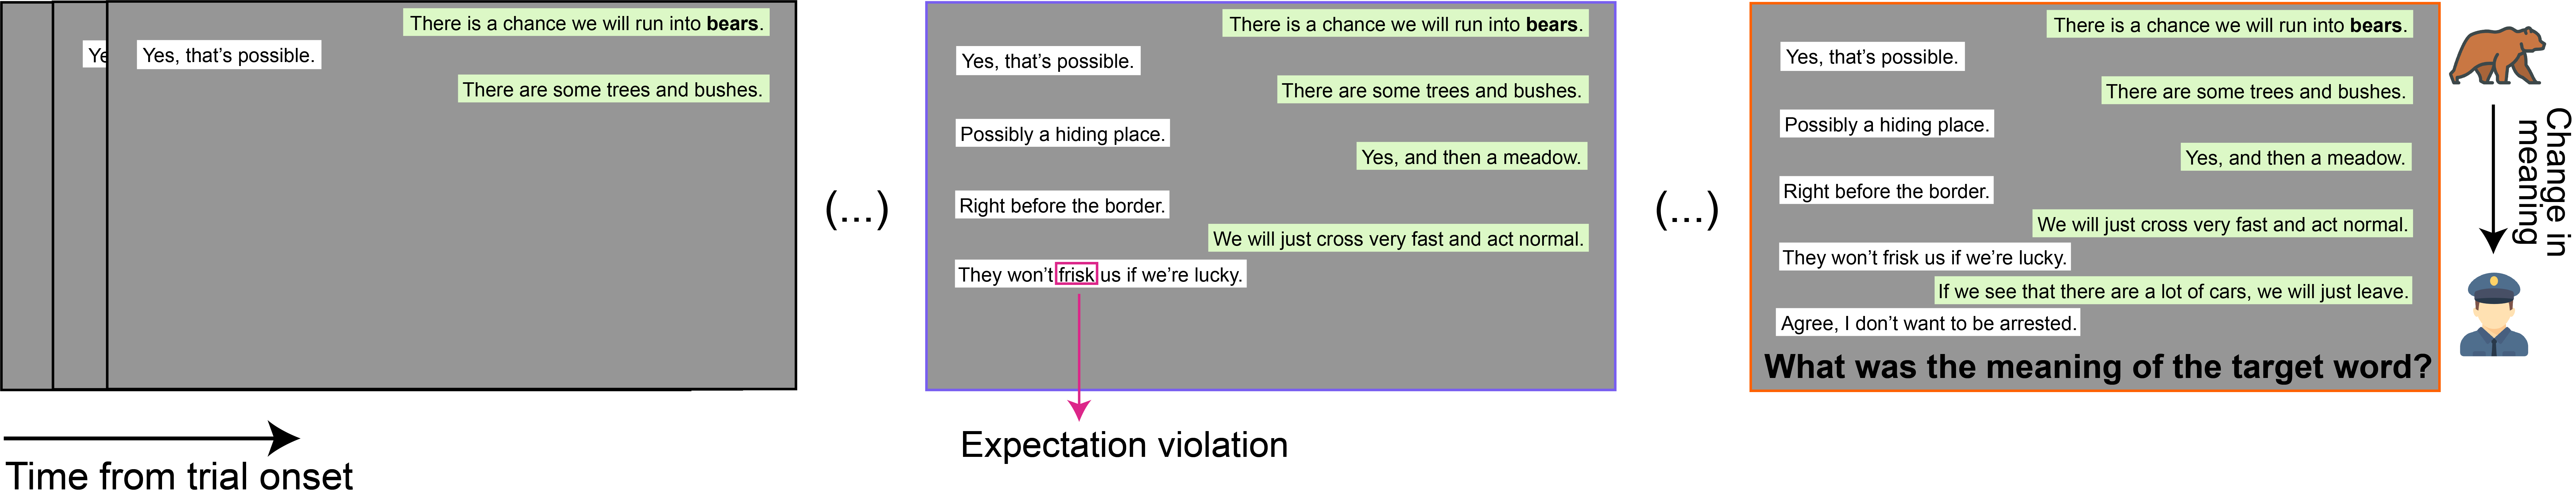
\includegraphics[width=1.1\textwidth, clip=true]{./Chapters/05_Discussion/Images/csi_image_horizontal}
	\caption{The NeuroCSI paradigm, which aims to probe the cognitive processes underlying the integration of context with utterance meaning. Participants read the chat conversation for which sentences appear on screen one at a time. In this example trial, the target word (\textit{bears}) has a different meaning (\textit{police}) than its literal meaning. The first sentence that could indicate that the target word has a slang meaning is the \textit{expectation violation} (see screen with purple outline), a critical event for analysis. After all sentences have appeared on screen, the participants decide on the meaning of the target word (see screen with orange outline). In these "slang" trials, the likely meaning of the target word has changed from its literal meaning to the slang meaning over the course of the dialogue and can be inferred from the context. }
    \vspace*{-10pt}
	\label{fig:csi}
\end{figure}

The design of this study uniquely combines language comprehension and mentalizing. On the one hand, participants have to make sense of the literal meaning of the messages in the dialogue and integrate each message with the unfolding context. On the other hand, when the literal meaning seems unlikely to fit the context, they must imagine what the interlocutors might mean with a possible slang target word. Based on the results in chapter~\ref{ch:language_asc}, I hypothesize that autistic and neurotypical people might perform equally well in trials where the intended meaning by the interlocutor matches the literal meaning. However, the decreased neural variability in autistic participants discussed in chapter~\ref{ch:mentalizing_asc} suggest that autistic individuals may focus more on the literal meaning of the dialogue and therefore show weaker or delayed integration of the intended meaning. The results of this upcoming study alongside those of the other chapters in this thesis will inform behavioral and neural theories on how autistic individuals integrate linguistic and social information into the interpretation of a signal \citep{wadge2019}. Difficulties in social interactions like context-inappropriate language use commonly influence connections and friendships for autistic people \citep{howlin2004,bauminger2003,bauminger2000}. For this reason, understanding the cognitive mechanisms underlying autistic communication is necessary to improve their well-being.

\section{Solving the puzzle of communication}

In chapters \ref{ch:mentalizing_asc} to \ref{ch:language_asc}, I have outlined experiments on mental state inferencing and linguistic structure building. While these are undeniably crucial pieces to solving the puzzle of communication, the single-person approach in which these experiments were conducted can only tell us so much about communication, an activity typically involving more than one person. This is for instance demonstrated by the finding that simply having another person present in a non-communicative task can affect a principal psycholinguistic process like lexical retrieval \citep{kuhlen2017having}. To see if these psycholinguistic and psychological abilities hold up in situations where more people are present, replicating these studies in a set-up with more than one person is important to validate the ecological validity of their effects.

A big part of the puzzle may be solved with new insights into communication in interactive settings. Psychology and language have primarily investigated their respective phenomena with participants engaging in a one-way interpretation of utterances or signals. This gives a one-sided view of the mind, since we acquire interests, fears, desires, and the meaning of concepts through others \citep{zaki2011,safran2014,defelice2023}. As briefly mentioned in chapter~\ref{ch:introduction}, understanding the dynamic, back-and-forth nature of communication calls for more insight into, firstly, the creative way in which interlocutors can create and use referents and words in dialogue. Introducing and using newly created terms to refer to people and objects can help define and clear up ideas, and in turn make sure you and the person you are speaking to are talking about the same thing or person \citep{brennan1996}. For example, if you have two friends named Alex, you might refer to one or both of them with a distinctive feature, like what they study, and call them \textit{Walex} (\underline{w}iskunde = mathematics) and \textit{Skalex} (\underline{s}cheikunde = chemistry). This process of reference creation and use is known as entrainment in the psycholinguistic literature \citep{brennan2010}. Preliminary evidence suggests that the right temporal lobe and ventromedial PFC are involved in producing and interpreting these new signals \citep{stolk2013neural}. To the same end, it is not just important what to say but also when to say it: responding in a timely manner is important for an enjoyable conversation and feelings of social connection with your conversational partner \citep{templeton2022}. Even more so, poorly timed responses carry (unintended) meaning. Think of a `no' uttered very fast in response to an invitation, which can come off as rude, or the exact opposite, a `yes' uttered slowly, possibly indicating unwillingness to accept a request \citep{bogels2015never,kendrick2015}. The existing neuroscientific evidence shows that this response planning starts already 500 ms after hearing the critical information in the conversation partner's utterance \citep{bogels2015neural}. These subtle and fleeting pieces of the communication puzzle show the mounting complexity of the problem in interactive settings and therefore warrant more investigation. 

Understanding the interactive aspect of communication is all the more important in autism and social anxiety, since the difficulties and frustrations of these individuals arise from interactive settings. Since autistic and socially anxious individuals struggle the most in unpredictable conversations \citep{roeyers2001,ponnet2008,pilkonis1977,thompson2002}, the most valuable insights are to be gained from experiments in unpredictable, interactive settings paired with tools to measure the underlying neural mechanisms of fleeting conversational dynamics. 

\section{Conclusion}

This thesis has described the neural mechanisms underlying mental state inferencing and language comprehension in autism and social anxiety. By examining mental state inferencing in a more naturalistic context our findings indicate, on the one hand, that autistic and neurotypical individuals have similar behavioral and neural responses. On the other hand, differences between the two groups are elicited in their neural variability in response to viewing social interactions. When comparing socially anxious and control participants in this way, decreased neural activation during mental state inferencing is found for socially anxious individuals in addition to differences in neural variability. Crucially, these differences were not due to anxiety during the experiment. When examining neural signatures of linguistic structure building, autistic and neurotypical individuals show similar neural measures on a reliably identified oscillatory component, as well as similar lateralization of this component. These insights indicate that the use of experimental set-ups that approximate everyday situations is a promising way of learning more about how neurotypical and neurodivergent understand language and communication. 
%\afterpage{\blankpage}
\chapter*{Appendix}
\chaptermark{Appendix} % uncomment for final version
\addcontentsline{toc}{chapter}{Appendix}
%\thispagestyle{empty}
\linespread{1}
\begin{small}
\bibliographystyle{apalike}
\cleardoublepage
\phantomsection
\addcontentsline{toc}{section}{Bibliography}
%\section*{Bibliography}
\bibliography{Bibliography/Bibliography}
\end{small}
\newpage
\phantomsection
\addcontentsline{toc}{section}{Research Data Management}
\section*{Research Data Management}
This research followed the applicable laws and ethical guidelines. Research Data Management was conducted according to the FAIR principles. The paragraphs below specify in detail how this was achieved.

\subsection*{Ethics}
This thesis is based on the results of human studies, which were conducted in accordance with the principles of the Declaration of Helsinki. The Ethical Committee of the faculty of Social Sciences (ECSS) has given a positive advice to conduct these studies to the Dean of the Faculty, who formally approved the conduct of these studies (CMO:2019/6059). This research is funded by Gravitation Grant 024.001.006 of the Language in Interaction Consortium from the Netherlands Organization for Scientific Research (NWO).

\subsection*{Findable Accessible}
The table below details where the data and research documentation for each chapter can be found on the Donders Repository (DR). All data archived as a Data Sharing Collection remain available for at least 10 years after termination of the studies.

\begin{table}[ht]
    \captionsetup{justification=raggedright, singlelinecheck=false, font = normal} % Left-align the caption
    \setlength{\tabcolsep}{15pt}
    \renewcommand{\arraystretch}{1.2} % Adjust row spacing (default is 1.0)
    \begin{tabular}{llll}
    \hline
    \textit{Chapter} & \textit{DAC} & \textit{DSC} & \textit{DSC License} \\
    \hline
    2 & 3025003.02\_119 & 3025003.02\_622 & CC0\-1.0 \\
    3 & 3025003.02\_119 & ??? & ??? \\
    4 & 3011225.01\_121 & ??? & ??? \\
    \hline
    \multicolumn{4}{l}{\small{Data Acquisition Collection, DSC = Data Sharing Collection}} \\
    \end{tabular}
\end{table}

Informed Consent was obtained through paper forms following the procedure of the Donders Centre for Cognitive Neuroimaging (DCCN). These forms are archived for 10 years in the central archive of the DCCN after termination of the studies. 
    
\subsection*{Interoperable, Reusable}
The raw data is stored on the DAC in the form it was acquired. The data of the DAC and DSC of chapter~\ref{ch:mentalizing_asc} and~\ref{ch:mentalizing_sa} have been organized according to BIDS standards. For DSC long-lived file formats (.csv, .txt) have been used ensuring that data remains usable in the future. Results are reproducible by providing a description of the experimental setup, raw data (DAC and DSC), analysis scripts or pipelines (DSC).

\subsection*{Privacy}
The privacy of the participants in this thesis has been warranted using random individual subject codes. A pseudonymization key linked this random code with the personal data. This pseudonymization key was encrypted with a password and stored on a network drive that was only accessible to members of the project who needed access to it because of their role in the project. The pseudonymization key was stored separately from the research data. Data in chapter~\ref{ch:mentalizing_asc} is not identifiable and shared without restrictions. The MRI data of chapter~\ref{ch:mentalizing_asc} is defaced.


\newpage
\phantomsection
\addcontentsline{toc}{section}{Dutch Summary}
\section*{Dutch Summary}

% intro
Om een goed gesprek te kunnen voeren, zijn in ieder geval twee vaardigheden noodzakelijk: het begrijpen van woorden en zinnen en het bedenken wat andere mensen geloven en denken. Die laatste vaardigheid wordt ook wel \emph{mentalizing} genoemd. Van beide vaardigheden is bekend dat ze minder goed ontwikkeld kunnen zijn in mensen met Autisme Spectrum Stoornis. Autistische mensen ervaren regelmatig problemen bij het houden van gesprekken in verbale en non-verbale communicatie. Autistische mensen lopen ook vaak achter in hun taalontwikkeling in vergelijking met niet-autistische mensen. Voor een lange tijd leek psychologisch onderzoek aan te tonen dat autistische mensen minder goed zijn in mentalizing dan niet-autistische mensen. Er zijn echter een aantal dingen aan te merken op de manier waarop veel van dit onderzoek is uitgevoerd. Veel experimenten zijn erg gekunsteld op een manier dat ze niet goed weergeven hoe mensen in de echte wereld nadenken over de gedachten en overtuigingen van een ander. Ook kan bij sommige experimenten het verminderde mentalizingniveau van autistische mensen verklaard worden door een andere factor, zoals taalvaardigheid van de proefpersonen. Bovendien tonen meer recente experimenten aan dat autistische mensen mentalizingtaken even goed volbrengen als niet-autistische mensen. Het was dus nog onduidelijk hoe deze twee groepen verschillen in mentalizing als dit onderzocht wordt in een meer re\"eele setting.

Een andere conditie waarbij mensen problemen ervaren tijdens communicatie is sociale angst, gekenmerkt door een ernstige angst om negatief beoordeeld te worden door anderen. Een gevolg hiervan kan zijn dat sociaal angstige mensen sociale situaties helemaal vermijden en zich isoleren. Een mogelijke verklaring voor deze angst is een verminderd mentalizingvermogen, wat leidt tot stress bij het proberen te interpreteren van het gedrag van anderen. Een andere verklaring is dat sociale cues en informatie anders binnenkomen bij sociaal angstige mensen en als het ware gemonitord worden voor mogelijke sociale dreigingen. Bij het testen van deze verklaringen stuiten we op dezelfde problemen als het onderzoek naar mentalizing in autisme. Daar bovenop komt ook nog dat sociaal angstige proefpersonen veel prestatiedruk kunnen ervaren tijdens een experiment waar ze telkens opdrachten krijgen om te voltooien. Het is dus belangrijk dat sociaal angstige proefpersonen tijdens een taak zo min mogelijk het gevoel hebben dat ze beoordeeld worden.

Om de communicatieproblemen in autistische en sociaal angstige mensen volledig te kunnen begrijpen en op zoek te gaan naar behandelingen is het van belang dat we kijken of er een biologische verklaring is voor hun klachten. Daarom hebben we in het onderzoek in dit proefschrift vooral gekeken naar de signalen in de hersenen terwijl autistische, sociaal angstige, en neurotypische (geen van beide condities) mensen taken deden zoals zinnen lezen of een video kijken waarin personages met elkaar communiceren. Op deze manier kunnen we aanknopingspunten vinden voor behandelingen of therapie die hun dagelijkse problemen kunnen verminderen. 

% chapter 2
In hoofdstuk~\ref{ch:mentalizing_asc} hebben we autistische en neurotypische mensen een video laten kijken waarin twee bevriende personages op een probleem stuiten en dat proberen op te lossen. Belangrijk is dat de video geen taal bevat, wat betekent dat verschillen in taalvaardigheid de resultaten niet kunnen be\"invloeden. Dit doen ze terwijl ze in een MRI-scanner (Magnetic Resonance Imaging) scanner liggen om hun hersensignalen te meten. Ook wordt hun pupilgrootte gemeten, wat een indicatie geeft hoeveel inspanning het vergt om een bepaald beeld of geluid te waarnemen en interpreteren. Na het kijken van de video beantwoordden ze een aantal vragen over de video. Als we de hersensignalen, pupilgroottes en beschrijvingen van de twee groepen vergelijken, zien we dat er geen verschillen zitten tussen de autistische en neurotypische proefpersonen in de mate waarin ze bedenken wat de gedachten van de personages inhouden. Wel zien we dat autistische proefpersonen over de hele video onderling meer wisselende hersenactiviteit laten zien, in vergelijking met de meer onderling vergelijkbare neurotypische proefpersonen. Dit ligt niet in lijn met andere, vergelijkbare studies. We denken dat dit mogelijk kan verklaard worden door eigenschappen van de specifieke video die gebruikt wordt in dit type experiment.

% chapter 3
Voor het onderzoeken van mentalizing en het interpreteren van sociale interacties in sociale angst hebben we in hoofdstuk~\ref{ch:mentalizing_sa} een vergelijkbare aanpak gebruikt als in hoofdstuk~\ref{ch:mentalizing_asc}. Sociaal angstige en niet sociaal angstige mensen keken dezelfde video als in hoofdstuk~\ref{ch:mentalizing_sa} in een MRI-scanner, waarbij we weer ge\"interesseerd waren in de reactie van de hersenen, de pupilgrootte en achteraf de beschrijvingen van de video. Cruciaal is dat de proefpersonen geen instructie kregen om vragen te beantwoorden om prestatiedruk te minimaliseren. In de data zagen we dat een klein gebied in het achterste deel van de linker temporale kwab minder actief was in sociaal angstige mensen bij het bekijken van scenes waarin de proefpersonen zich sterk zouden inleven in de personages. Dit gebied is vaak betrokken bij het interpreteren van binnenkomende sociale cues in het licht van sociale kennis die je al bezit, wat dus verzwakt zou kunnen zijn in sociaal angstige mensen. Als we kijken naar hoe wisselend de hersenactiviteit tussen proefpersonen is binnen dezelfde groep, zien we dat bepaalde stukken van de film en hersengebieden zowel meer als minder wisselend zijn in sociaal angstige mensen in vergelijking met niet sociaal angstige mensen. Dit wijst erop dat er een mogelijke automatische bias is in het verwerken van sociale cues in sociaal angstige mensen die hun andere manier van denken kan verklaren. 

% chapter 4
Vanwege de veelvoorkomende vertragingen in taalontwikkeling in autisme hebben we in hoofdstuk~\ref{ch:language_asc} onderzocht hoe de hersensignalen eruit zien als autistische en neurotypische mensen zinnen proberen te begrijpen. Er is namelijk nog niet eerder onderzoek gedaan naar de vraag of zinsopbouw anders verwerkt wordt in de hersenen en vooral of bepaalde signalen eerder of later plaatsvinden. In dit experiment lazen de twee groepen proefpersonen zinnen met of zonder zinstructuur terwijl hun hersengolven werd gemeten met EEG (Electroencephalography). De resultaten bevestigden eerder onderzoek dat hersengolven in de beta band (14 - 20 Hz) een goede signatuur bleken van het verwerken van zinsopbouw, maar deze en andere hersengolven lieten dezelfde patronen zien in autistische en neurotypische proefpersonen. Op basis van eerder onderzoek met een andere methode waren we ook ge\"interesseerd of de hersengolven even sterk aanwezig waren in beide hersenhelften. Dit was het geval, en bovendien niet verschillend tussen de twee proefpersoongroepen of over de tijd heen die het kostte om een zin te lezen.

% conclusion
De bevindingen in dit proefschrift laten zien dat eerder beschreven verschillen tussen autistische en neurotypische personen niet universeel aanwezig zijn in alle autistische personen. We weten nu dus dat het onjuist is om te praten over een algemene tekortkoming in het mentalizingvermogen van autistische personen. Ook zijn veelgenoemde neurale kenmerken tijdens taalbegrip in autisme niet altijd aangetast. Verder hebben we ontdekt dat het nuttig is om mentale vaardigheden opnieuw te testen in een setting die meer overeenkomen met hoe deze in de echte wereld toegepast worden. Hiermee hebben we in autisme en sociale angst aangetood dat mentalizingvermogen en het interpreteren van social interacties anders kan zijn dan aanvankelijk bekend was. Meer kennis over de specifieke aspecten die sociale informatie interpreteren anders maakt in deze condities is noodzakelijk voor een beter begrip hierover, waarvoor het onderzoek in dit proefschrift een weg heeft kunnen banen.

%\newpage
%\section{Biography}
\addcontentsline{toc}{chapter}{Biography}
Tim van Mourik was born on September 27th 1990 in Leiden, the Netherlands. After graduating from the Stedelijk Gymnasium Leiden, he went on to pursue a Bachelor's degree in the exact sciences at the Roosevelt Academy (currently: University College Roosevelt). After this, he enrolled in the Master Computer Animation and Visual Effects at Bournemouth University. Over the course of this program, he started to develop an interest in medical image processing and completed the program with an internship at the Donders Centre for Cognitive Neuroimaging under the supervision of prof. David Norris. As MRI scanners operate on physical and mathematical principles, subsequently producing three-dimensional images, this perfectly combined Tim's expertises and interests. He continued to work as a research assistant at the Donders Institute where he was initiated in the world of neuroimaging and laminar analysis. In February 2014, he started a four-year PhD project to investigate and better understand the cortical layers of the brain. During this time he developed methods for better analysing laminar fMRI data and under the supervision of Dr. Janneke Jehee, he conducted a study on the layer specificity of spatial attention. All tools, code, and data for his published work is openly available, as Tim is a strong proponent of open science, data and code sharing, and open source development. In this spirit, he programmed worfklow software, Porcupine, that automatically and more transparently creates analysis code. He is currently contuining this line of work by creating an online platform for easier data sharing, GiraffeTools. It is unknown where he acquired his peculiar taste for silly acronyms. For these efforts towards open science he was elected to be the chair of the Open Science Room at OHBM 2019, Rome. 

%\newpage
%\section{Author publications}
\addcontentsline{toc}{chapter}{Author publications}
\vspace{20pt}
\subsection{Published papers}
\vspace{10pt}
\hangindent=2em
\noindent
% Author
{\textbf{T.~van Mourik}, L.~Snoek, T.~Knapen, and D.~Norris.} 
% Year
(2018).
% Title
Porcupine: a visual pipeline tool for neuroimaging analysis.
% Journal
\emph{PLoS computational biology.}


\hangindent=2em
\noindent
% Author
{S.~Lawrence, \textbf{T.~van Mourik}, P.~J. Koopmans, D.~Norris, and F.~de~Lange.} 
% Year
(2018).
% Title
Laminar Organization of Working Memory Signals in Human Visual Cortex. 
% Journal
\emph{Current Biology, in press.}


\hangindent=2em
\noindent
% Author
{N.~Z.~Bielczyk, S.~Uithol, \textbf{T.~van Mourik}, P.~Anderson, J.~C.~Glennon, and J.~K.~Buitelaar} 
% Year
(2018).
% Title
Disentangling causal webs in the brain using functional Magnetic Resonance Imaging: A review of current approaches.
% Journal
\emph{Network Neuroscience.}


\hangindent=2em
\noindent
% Author
{R.~Scheeringa, P.~J.~Koopmans, \textbf{T.~van Mourik}, D.~Norris, and Jensen.} 
% Year
(2016).
% Title
The relationship between oscillatory {EEG} activity and the laminar-specific bold signal.
% Journal
\emph{PNAS.}


\hangindent=2em
\noindent
% Author
{P.~Kok, L.~Bains, \textbf{T.~van Mourik}, D.~Norris, and F.~de~Lange.} 
% Year
(2016).
% Title
Selective activation of the deep layers of the human primary visual	cortex by top-down feedback.
% Journal
\emph{Current Biology.}


\hangindent=2em
\noindent
% Author
{M.~Kleinnijenhuis, \textbf{T.~van Mourik}, D.~G. Norris, D.~J. Ruiter, A.-M. van	Cappellen~van Walsum, and M.~Barth.} 
% Year
(2015).
% Title
Diffusion tensor characteristics of gyrencephaly using high	resolution diffusion {MRI} in vivo at 7{T}.
% Journal
\emph{NeuroImage.}

\vspace{10pt}

\subsection{Publications in preparation}
\vspace{10pt}
\hangindent=2em
\noindent
% Author
{\textbf{T.~van Mourik}, P.~J. Koopmans, L.~J. Bains, D.~G. Norris, and J.~F. Jehee.} 
% Title
Investigation of layer specific bold during visual attention in the human visual cortex.
% Journal
\emph{In preparation.}


\hangindent=2em
\noindent
% Author
{\textbf{T.~van Mourik}, P.~J. Koopmans, L.~J. Bains, and D.~G. Norris.} 
% Title
Improved cortical boundary registration for locally distorted fMRI scans.
% Journal
\emph{Submitted, Preprint on bioRxiv.}


\hangindent=2em
\noindent
% Author
{\textbf{T.~van Mourik}, J.~P.~J.~M.~ van der Eerden, P-L.~Bazin, D.~G. Norris.} 
% Year
(2018).
% Title
Laminar signal extraction over extended cortical areas by means of a spatial GLM.
% Journal
\emph{Submitted, Preprint on bioRxiv.}


\hangindent=2em
\noindent
% Author
{F.~Molaei-Vaneghi, N.~Zaretskaya, \textbf{T.~van Mourik}, J.~Bause, K.~Scheffler, and A.~Bartels.} 
% Title
9.4 T Human fMRI Study Reveals that Real World Motion Perception Does Not Involve Laminar Organization in V1 and V5/MT.
% Journal
\emph{Submitted.}


\hangindent=2em
\noindent
% Author
{S.~H.~P.~Collin, P.~van den Broek, \textbf{T.~van Mourik}, P.~Desain, C.~F.~Doeller.}
% Title
Creating an artificial memory context alters associative memory formation.
% Journal
\emph{In preparation.}

%\newpage
%\section{Acknowledgements}
\addcontentsline{toc}{chapter}{Acknowledgements}

Over the six years that I spent working at the Donders Institute I have met so many people without whom this thesis would not be what it is today. I cannot do justice to all of you but I will at least try for a small subset.

%%%%%% David
First, I would like to thank my supervisor and promotor David Norris. When I came in as a student of the exact sciences I preferred to put \emph{quod erat demonstrandum} at the end of every paragraph. You taught me a lot about the scientific method in neuroscience, bigger pictures and the gran(d/t) scheme of things, the politics of laminar analysis, and many other things. We took on Bert and Ernie roles in meetings: your blue sky thinking against my attempts to narrow ideas down to realisitic solution. Although the latter may come across as pessimistic, I believe it often resulted in an efficient and pragmatic middle-ground. I am thankful for the amount of dedication and personal attention you give to your students, while still having them to express their autonomy to become an independent researcher.

%%%%%% Janneke
I would especially like to thank my co-promotor Janneke Jehee. Visual computation, so I found out, has nothing to do with visual effects, and also not so much with computers. My very first email to the Donders Institute was to inquire about a position in your lab. But you kindly explained that the computations of the visual cortex might not suit my interest or skillset and referred me to the head of the MR physics lab. It was years later that our paths crossed again when you took me up in your lab when I wanted to study layers in the visual cortex. I am very grateful for the time and dedication with which you helped me to conduct this study from beginning to (pending) end. I truly admire your dedication and resilience; your extreme precision with words, analysis, and way of doing science. The time that I spent in your lab has not been able to hook me on the workings of the visual cortex, but it has certainly broadened my horizon and made me a better scientist, for which I am very grateful.

%%%%%% The FAD
When I started as a research assistant, there was still a dedicated culture of Friday Afternoon Drinks. From the very first week on, this made me feel welcome at the Donders and familiarised me in no time with Romagna and all real restaurants in Nijmegen. And fortunately it was not all too often that this resulted in knife fights over a glass of white wine. Although the old gang has left the building (save some Donders dinosaurs),  the FAD still remains, and I would like to thank everybody with whom I have conversations and discussions that brightened up my Friday afternoon.

%%%%%% The Kitchen
Thanks to everybody in the kitchen, the old kitchen and the new canteen, for a countless number of lunches, coffees, random cake days (and those rare random suit-up days), and much more. Whether the topic of the day was general linear models, the state of science, of the world, of Brexit, or just pink elephants and the order of the day, I appreciated the diverse and stimulating environment. Over the last six years the Donders grew out from a village to a city, with all its infrastructural perks, but it lost some of its the `market square' like atmosphere in the kitchen. ``Having only a single, slow coffee machine in a research institute is an underappreciated method for enhancing interdisciplinary collaboration'' (Mostert 2016).

%%%%%% Lab group
I would like to thank my lab group for the feedback on layers and porcupines, for sharing frustrations over rejection in the info-meeting, and for the historical geo-political discussion in the group lunches.

%%%%%% Office mates
Thanks to all office mates that I had over the years. For the company, the \emph{boekje-bijna-klaar?} encouragements, sharing in the MATLAB frustrations, the Armin moments on Friday afternoon (before the FAD of course), and much more. 
 
%%%%%% Admin
The backbone of the Donders is formed, of course, by Tildie, Ayse and the administration, Marek and the minions, and `koning-van-de-kelder' Paul. Thank you for all the help and support, and making everything run smoothly. We all know that the Donders would collapse without you. 

%%%%%% Vierkant
There is always one special week per year reserved for Vierkant, the maths puzzle camp, in which I do not think about MRI scanners at all. Thanks to all Vierkanters for this exciting and stimulating week, for the random sketches, for each one of you to bring your own kind of crazyness along. 

%%%%%% Paranymphs & family 
Thanks to my dear paranymphs, Tom, Jelle, and Annelies, for all the support along the way. Not just for the home stretch, but primarily in all the preceding years. You have been a sounding board for many a wonky idea that eventually made it to this thesis. A special thanks to my parent and my brothers, who may not always have understood what I have been doing all these years, but still unconditionally supported me doing it and showing genuine interest. And thanks for the the sailing trips, expert advice on vegetable gardens, conversations about balloon warriors, and much more. 

%%%%%% Tineke
Dear Tineke, my Queen of Hearts, occupational panda and occasional sloth. Acronym expert, kindest supporter, and toughest critic. It is quite unclear where we will end up next, but it will be somewhere together. 





%\newpage
%
\section{Donders Graduate School for Cognitive Neuroscience}

For a successful research Institute, it is vital to train the next generation of young scientists. To achieve this goal, the Donders Institute for Brain, Cognition and Behaviour established the Donders Graduate School for Cognitive Neuroscience (DGCN), which was officially recognised as a national graduate school in 2009. The Graduate School covers training at both Master's and PhD level and provides an excellent educational context fully aligned with the research programme of the Donders Institute.

The school successfully attracts highly talented national and international students in biology, physics, psycholinguistics, psychology, behavioral science, medicine and related disciplines. Selective admission and assessment centers guarantee the enrolment of the best and most motivated students.

The DGCN tracks the career of PhD graduates carefully. More than 50\% of PhD alumni show a continuation in academia with postdoc positions at top institutes worldwide, e.g. Stanford University, University of Oxford, University of Cambridge, UCL London, MPI Leipzig, Hanyang University in South Korea, NTNU Norway, University of Illinois, North Western University, Northeastern University in Boston, ETH Z\"urich, University of Vienna etc. Positions outside academia spread among the following sectors: specialists in a medical environment, mainly in genetics, geriatrics, psychiatry and neurology. Specialists in a psychological environment, e.g. as specialist in neuropsychology, psychological diagnostics or therapy. Positions in higher education as coordinators or lecturers. A smaller percentage enters business as research consultants, analysts or head of research and development. Fewer graduates stay in a research environment as lab coordinators, technical support or policy advisors. Upcoming possibilities are positions in the IT sector and management position in pharmaceutical industry. In general, the PhDs graduates almost invariably continue with high-quality positions that play an important role in our knowledge economy.

For more information on the DGCN as well as past and upcoming defenses please visit: 

\url{https://www.ru.nl/donders/graduate-school/phd}




%\afterpage{\blankpage}

\end{document}
